\documentclass
% [draft=true]
{beamer}
\usepackage[utf8]{inputenc}
\usecolortheme{orchid}
\usepackage{fontawesome5}
\usepackage{adjustbox} % in preamble
\usepackage{pifont} 
\usepackage{nicefrac}
\usepackage{csquotes}
\usepackage{graphicx}
\usepackage{changepage} 
\usepackage{cancel}  

%hide table column
\usepackage{array} \newcolumntype{H}{>{\setbox0=\hbox\bgroup}c<{\egroup}@{}}

\def\checkmark{\resizebox{0.1\textwidth}{!}{\tikz\fill[scale=0.4](0,.35) -- (.25,0) -- (1,.7) -- (.25,.15) -- cycle;}}
\usepackage{tikz}
\usetikzlibrary{shapes.geometric, arrows.meta, positioning}
\usetikzlibrary{positioning,arrows}
\usepackage[dvipsnames]{xcolor}
\makeatletter
\def\blfootnote{\gdef\@thefnmark{}\@footnotetext}
\makeatother
\newcommand{\crossout}[2][red]{%
  \begin{tikzpicture}[baseline=(texte.base)]
    % Nœud pour le texte
    \node[inner sep=0pt, outer sep=0pt] (texte) {#2};
    % Dessiner la croix (deux lignes diagonales)
    \draw[overlay, #1, line width=0.5pt] 
      (texte.north west) -- (texte.south east); % Ligne diagonale 1
    \draw[overlay, #1, line width=0.5pt] 
      (texte.north east) -- (texte.south west); % Ligne diagonale 2
  \end{tikzpicture}%
}
\setbeamertemplate{navigation symbols}{}
\usepackage[  
backend=biber,
% style=alphabetic, 
]{biblatex} 
\addbibresource{../../bib/these.bib}
\usepackage{xcolor, cmbright,diagbox,colortbl,tikz,graphicx,algorithm2e,cancel,verbatim, graphicx,
listings,float,amsmath,amssymb,array,subfiles,bussproofs,
rotating,MnSymbol,mathtools,subcaption,caption}
\newtheorem{proposition}{Proposition}
\usetikzlibrary{overlay-beamer-styles}
\usetikzlibrary{automata, positioning,graphs,shapes, arrows, calc}

\newcommand{\set}[1]{\{#1\}}
\newcommand{\vertex}[2]{%
  \begin{tikzpicture}[baseline=-1ex]%
    \node [rectangle,rounded corners=2mm,inner sep=0.5mm,fill=#2] {$#1$};%
  \end{tikzpicture}%
}
\newcommand{\graphbox}[8]{
  \begin{scope}[xshift=#2,yshift=#3]
    \draw [rounded corners=2mm] (0,0) rectangle (#4,-#5);
    \node at (0,0mm) [anchor=north west,inner sep=1mm] {#1};
    \begin{scope}[xshift=#4/2+#6,yshift=#7] 
    #8
    \end{scope}
  \end{scope}
}

\newcommand{\opn}[1]{\operatorname{#1}}

\graphicspath{ {.} }
\usepackage{hyperref}
\title{Automated Termination Proving: Contributions to Graph Rewriting\\via Extended Weighted Type Graphs\\and Morphism Counting}
\setbeamertemplate{footline}[frame number]

\usetheme{default}
\begin{document}
\date{\today}
\date{}
\author{Qi QIU}
\institute[VFU] % (optional)
{
    LIRIS, UMR 5205 CNRS\\
	Université Claude Bernard Lyon 1, France\\
    Supervisor: Xavier URBAIN\\
}

\titlegraphic{%
  \includegraphics[height=1.2cm]{logo_liris.png}\hspace{5mm}%
  \includegraphics[height=1.5cm]{logo_lyon1.jpg}%
}

\maketitle
\note{  
    Bonjour a tous, je vous remercie pour votre presence.
    Aujourd'hui, je vais vous presenter mes travaux de these. 
    8s
}
\begin{frame}{Motivation \& Goal} 

    \begin{description} 
        \item[Distributed systems:]\ \\
            \resizebox{0.3\textwidth}{!}{
            \begin{tikzpicture}
                \node (n1) at (-1.2,0) {\faIcon{laptop-code}};
                \node (n2) at (0,1.2) {\faIcon{laptop-code}};
                \node (n3) at (1.2,0) {\faIcon{laptop-code}};
                \node (n4) at (0,-1.2) {\faIcon{laptop-code}};
                \draw[-] (n1) -- (n2);
                \draw[-] (n2) -- (n3);
                \draw[-] (n3) -- (n4);
                \draw[-] (n4) -- (n1);
                \draw[-] (n1) -- (n3);
                \draw[-] (n2) -- (n4);
            \end{tikzpicture}
            }
        \item[Failures can be catastrophic:]                
            %   \faIcon{laptop-code}
            %   \faIcon{mobile-alt}
              \faIcon{medkit}
              \faIcon{train}
              \faIcon{plane}
              \faIcon{rocket} 
        \item[Ensuring correctness is difficult.]\ \\
            \begin{itemize}
                \item Needham-Schroeder protocol shown to be vulnerable 17 years after publication
                % \item Distributed algorithms are complex.
                % \item Human proofs are error-prone.
            \end{itemize}
        \item[This thesis: automated verification]\ \\
            \begin{itemize}
                \item Minimal user effort
                \item No expertise required
                \item Mathematically rigorous
            \end{itemize}
    \end{description}
\note{
Ma thèse s'intéresse aux algorithmes distribués.
Ils permettent à plusieurs machines indépendantes de réaliser une tâche commune. Les machines communiquent entre elles via messages.

Des conséquences catastrophiques peuvent survenir en cas de défaillance, car ces algorithmes sont largement utilisés dans les systèmes médicaux et de transport.

Cependant, assurer la correction de ces systemes est difficile.
Par exemple, un protocole d'authentification a été prouvée vulnérable 17 ans après sa publication.

Cette thèse vise à proposer des méthodes rigoureuses et automatiques de vérification des systèmes distribués pour minimiser l'effort de l'utilisateur et ne pas requérir d'expertise particulière.

1m30
keywords: independant; vise à reduire
}
\end{frame}

 
\begin{frame}{Graph Transformation: Intuition}
Modeling of distributed systems
 \newline\newline
 System configurations: graphs
    \begin{center}
             \begin{tikzpicture}[scale=0.9]
                \node (n2) at (1,1) {\faIcon{laptop-code}};
                \node (n4) at (1,-1) {\faIcon{laptop-code}};
                \node (n3) at (2,0) {\faIcon{laptop-code}};
                \node (n5) at (3,-1) {\faIcon{laptop-code}};
                \node (n6) at (3,1) {\faIcon{laptop-code}};
                \node (n1) at (0,0) {\faIcon{laptop-code}};
                \draw (n1)--(n2);
                \draw (n2)--(n3)--(n4);
                \draw (n4)--(n1);
                \draw (n3)--(n6);
                \draw (n6)--(n5);
                \draw (n5)--(n3);
                \phantom{            
                    \draw[red, dashed, very thick] (0,0) circle (1.65);
                }
            \end{tikzpicture}
            \hspace{0.1\textwidth}
        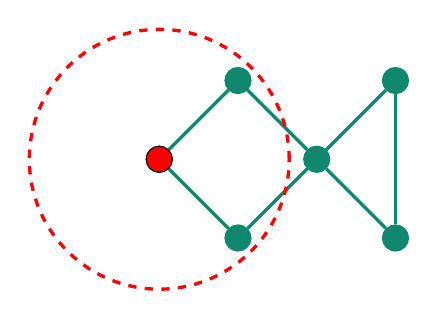
\begin{tikzpicture}
            \node[fill=PineGreen, PineGreen,draw, circle] (n1) at (0,0) {};
            \node[draw, circle,fill=red] (n1) at (0,0) {};
            \node[fill=PineGreen, PineGreen,draw, circle] (n2) at (1,1) {};
            \node[fill=PineGreen, PineGreen,draw, circle] (n4) at (1,-1) {};
            \node[fill=PineGreen, PineGreen,draw, circle] (n3) at (2,0) {};
            \node[fill=PineGreen, PineGreen,draw, circle] (n5) at (3,-1) {};
            \node[fill=PineGreen, PineGreen,draw, circle] (n6) at (3,1) {};

            \draw[very thick, fill=PineGreen, PineGreen,-] (n1)--(n2);
            \draw[very thick, fill=PineGreen, PineGreen,-] (n2)--(n3)--(n4);
            \draw[very thick, fill=PineGreen, PineGreen,-] (n4)--(n1);
            \draw[very thick, fill=PineGreen, PineGreen,-] (n3)--(n6);
            \draw[very thick, fill=PineGreen, PineGreen,-] (n6)--(n5);
            \draw[very thick, fill=PineGreen, PineGreen,-] (n5)--(n3);
            \draw[very thick, red, dashed, very thick] (0,0) circle (1.65);
        \end{tikzpicture}
    \end{center}
 Algorithm behavior:

 \hspace{2cm}graph transformation based on 
\begin{tikzpicture}[baseline=-1ex]
            \node () at (0,0) {\text{local}};
            \draw[red, dashed, very thick] (0,0) circle (0.5);
        \end{tikzpicture} knowledge  

    \note{
On utilise la transformation de graphes pour modéliser les systèmes distribués.

Une configuration du système est représentée par un graphe : les nœuds représentent les unités de calcul et les arêtes représentent les canaux de communication entre ces unités.

Le comportement du système est représenté par une transformation du graphe, appliquée en fonction de la connaissance locale de certains nœuds.

(1 min)
    }
\end{frame}

\begin{frame}{Graph Transformation: Spanning-tree Construction}
    Graph transformation rule:
        \begin{center}
        \resizebox{0.7\textwidth}{!}{
            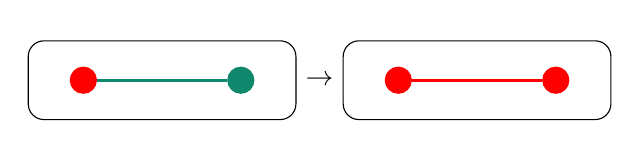
\begin{tikzpicture}
                        \graphbox{\(\)}{0mm}{0mm}{34mm}{10mm}{-10mm}{-5mm}{
                            \node[red,fill=red,draw, circle] (x) at (0,0) {};
                            \node () at (0,0.55) {};  
                            \node[PineGreen,fill=PineGreen,draw, circle] (y) at (2,0) {};
                            \node () at (2,0.55) {};
                            \draw[very thick, PineGreen,-] (x) -- node[midway,above] {} (y) ;
                            %             \draw[->] (x) edge [loop above] node {$A$} (x);
                            % \draw[->] (y) edge [loop above] node {$N$} (y);
                        }
                        \graphbox{\(\)}{40mm}{0mm}{34mm}{10 mm}{-10mm}{-5mm}{
                            \node[red,fill=red,draw, circle]  (x) at (0,0) {};  
                            \node () at (0,0.55) {};  
                            \node[red,fill=red,draw, circle]  (y) at (2,0) {};
                            \node () at (2,0.55) {};
                            \draw[very thick, red,-] (x) -- node[midway,above] {} (y) ;
                            % \draw[->] (x) edge [loop above] node {$A$} (x);
                            % \draw[->] (y) edge [loop above] node {$A$} (y);
                        }  
                        \node () at (37mm,-5mm) {\( \mathop{\rightarrow} \)}; % K -> L
            \end{tikzpicture}
        } 
        \end{center}
        Replace the left-hand side with the right-hand side
        \newline\newline
        % Spanning-tree construction:
        Application of the rule while possible:
    \begin{overlayarea}{\textwidth}{\textheight}
        \begin{center}
            \begin{onlyenv}<1>
            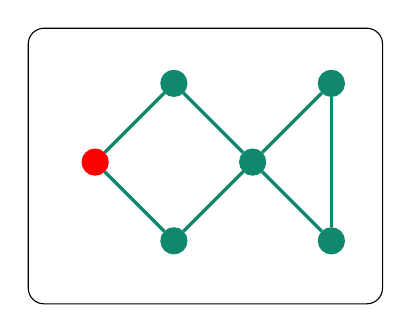
\begin{tikzpicture}
            \graphbox{}{0mm}{0mm}{45mm}{35mm}{-14mm}{-17mm}{
            \node[red,fill=red,draw, circle] (n1) at (0,0) {};
            \node[PineGreen,fill=PineGreen,draw, circle] (n2) at (1,1) {};
            \node[PineGreen,fill=PineGreen,draw, circle] (n3) at (2,0) {};
            \node[PineGreen,fill=PineGreen,draw, circle] (n4) at (1,-1) {};
            \node[PineGreen,fill=PineGreen,draw, circle] (n5) at (3,-1) {};
            \node[PineGreen,fill=PineGreen,draw, circle] (n6) at (3,1) {};
            \draw[very thick, PineGreen,-] (n1)-- node[pos=0.6, left] {} (n2);
            \draw[very thick, PineGreen,-] (n2)-- node[pos=0.35,right] {} (n3);
            \draw[very thick, PineGreen,-] (n3)-- node[pos=0.6,right] {}(n4);
            \draw[very thick, PineGreen,-] (n4)-- node[pos=0.45,left] {}(n1);
            \draw[very thick, PineGreen,-] (n3)-- node[pos=0.65,left] {}(n6);
            \draw[very thick, PineGreen,-] (n6)-- node[pos=0.4,right] {}(n5);
            \draw[very thick, PineGreen,-] (n5)-- node[pos=0.4,left] {}(n3);
            }
        \end{tikzpicture}
        % } 
        \end{onlyenv}
        \begin{onlyenv}<2>
               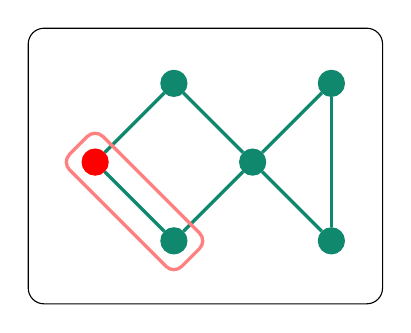
\begin{tikzpicture}
            \graphbox{}{0mm}{0mm}{45mm}{35mm}{-14mm}{-17mm}{
            \node[red,fill=red,draw, circle] (n1) at (0,0) {};
            \node[PineGreen,fill=PineGreen,draw, circle] (n2) at (1,1) {};
            \node[PineGreen,fill=PineGreen,draw, circle] (n3) at (2,0) {};
            \node[PineGreen,fill=PineGreen,draw, circle] (n4) at (1,-1) {};
            \node[PineGreen,fill=PineGreen,draw, circle] (n5) at (3,-1) {};
            \node[PineGreen,fill=PineGreen,draw, circle] (n6) at (3,1) {};
            \draw[very thick, PineGreen,-] (n1)-- node[pos=0.6, left] {} (n2);
            \draw[very thick, PineGreen,-] (n2)-- node[pos=0.35,right] {} (n3);
            \draw[very thick, PineGreen,-] (n3)-- node[pos=0.6,right] {}(n4);
            \draw[very thick, PineGreen,-] (n4)-- node[pos=0.45,left] {}(n1);
            \draw[very thick, PineGreen,-] (n3)-- node[pos=0.65,left] {}(n6);
            \draw[very thick, PineGreen,-] (n6)-- node[pos=0.4,right] {}(n5);
            \draw[very thick, PineGreen,-] (n5)-- node[pos=0.4,left] {}(n3);
             \draw[very thick, red!50, rounded corners,rotate around={45:(0,-0.5)}] ($(n4)+(-0.3,-0.3)$) rectangle ($(n1)+(0.3,0.3)$); 
            }
        \end{tikzpicture}
        \end{onlyenv}
         \begin{onlyenv}<3>
               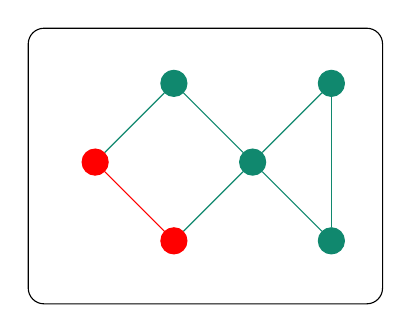
\begin{tikzpicture}
            \graphbox{}{0mm}{0mm}{45mm}{35mm}{-14mm}{-17mm}{
            \node[red,fill=red,draw, circle] (n1) at (0,0) {};
            \node[PineGreen,fill=PineGreen,draw, circle] (n2) at (1,1) {};
            \node[PineGreen,fill=PineGreen,draw, circle] (n3) at (2,0) {};
            \node[red,fill=red,draw, circle] (n4) at (1,-1) {};
            \node[PineGreen,fill=PineGreen,draw, circle] (n5) at (3,-1) {};
            \node[PineGreen,fill=PineGreen,draw, circle] (n6) at (3,1) {};
            \draw[PineGreen,-] (n1)-- node[pos=0.6, left] {} (n2);
            \draw[PineGreen,-] (n2)-- node[pos=0.35,right] {} (n3);
            \draw[PineGreen,-] (n3)-- node[pos=0.6,right] {}(n4);
            \draw[red,-] (n4)-- node[pos=0.45,left] {}(n1);
            \draw[PineGreen,-] (n3)-- node[pos=0.65,left] {}(n6);
            \draw[PineGreen,-] (n6)-- node[pos=0.4,right] {}(n5);
            \draw[PineGreen,-] (n5)-- node[pos=0.4,left] {}(n3);
            }
        \end{tikzpicture}
        \end{onlyenv}
        \begin{onlyenv}<4>
               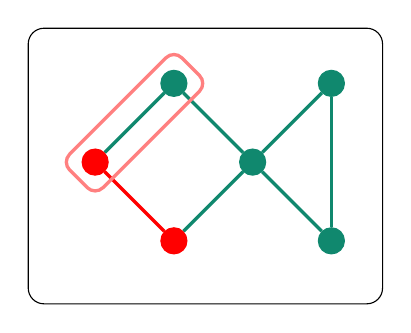
\begin{tikzpicture}
            \graphbox{}{0mm}{0mm}{45mm}{35mm}{-14mm}{-17mm}{
            \node[red,fill=red,draw, circle] (n1) at (0,0) {};
            \node[PineGreen,fill=PineGreen,draw, circle] (n2) at (1,1) {};
            \node[PineGreen,fill=PineGreen,draw, circle] (n3) at (2,0) {};
            \node[red,fill=red,draw, circle] (n4) at (1,-1) {};
            \node[PineGreen,fill=PineGreen,draw, circle] (n5) at (3,-1) {};
            \node[PineGreen,fill=PineGreen,draw, circle] (n6) at (3,1) {};
            \draw[very thick, PineGreen,-] (n1)-- node[pos=0.6, left] {} (n2);
            \draw[very thick, PineGreen,-] (n2)-- node[pos=0.35,right] {} (n3);
            \draw[very thick, PineGreen,-] (n3)-- node[pos=0.6,right] {}(n4);
            \draw[very thick, red,-] (n4)-- node[pos=0.45,left] {}(n1);
            \draw[very thick, PineGreen,-] (n3)-- node[pos=0.65,left] {}(n6);
            \draw[very thick, PineGreen,-] (n6)-- node[pos=0.4,right] {}(n5);
            \draw[very thick, PineGreen,-] (n5)-- node[pos=0.4,left] {}(n3);
            \draw[very thick, red!50, rounded corners,rotate around={45:(0,-0.5)}] ($(n1)+(-0.3,-0.3)$) rectangle ($(n2)+(0.3,0.3)$); 
            }
        \end{tikzpicture}
        \end{onlyenv}
        \begin{onlyenv}<5>
               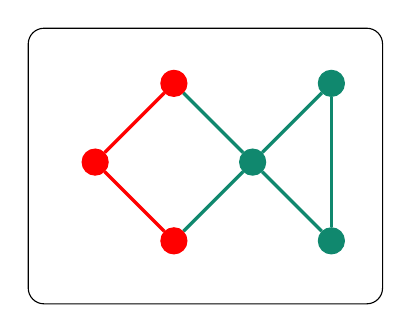
\begin{tikzpicture}
            \graphbox{}{0mm}{0mm}{45mm}{35mm}{-14mm}{-17mm}{
            \node[red,fill=red,draw, circle] (n1) at (0,0) {};
            \node[red,fill=red,draw, circle] (n2) at (1,1) {};
            \node[PineGreen,fill=PineGreen,draw, circle] (n3) at (2,0) {};
            \node[red,fill=red,draw, circle] (n4) at (1,-1) {};
            \node[PineGreen,fill=PineGreen,draw, circle] (n5) at (3,-1) {};
            \node[PineGreen,fill=PineGreen,draw, circle] (n6) at (3,1) {};
            \draw[very thick, red,-] (n1)-- node[pos=0.6, left] {} (n2);
            \draw[very thick, PineGreen,-] (n2)-- node[pos=0.35,right] {} (n3);
            \draw[very thick, PineGreen,-] (n3)-- node[pos=0.6,right] {}(n4);
            \draw[very thick, red,-] (n4)-- node[pos=0.45,left] {}(n1);
            \draw[very thick, PineGreen,-] (n3)-- node[pos=0.65,left] {}(n6);
            \draw[very thick, PineGreen,-] (n6)-- node[pos=0.4,right] {}(n5);
            \draw[very thick, PineGreen,-] (n5)-- node[pos=0.4,left] {}(n3);
            }
        \end{tikzpicture}
        \end{onlyenv}
        \begin{onlyenv}<6>
               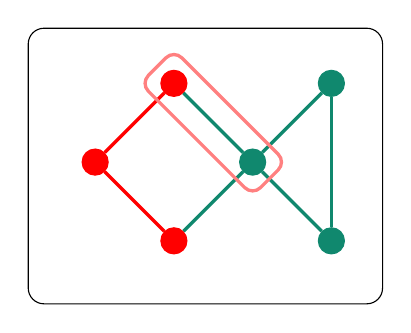
\begin{tikzpicture}
            \graphbox{}{0mm}{0mm}{45mm}{35mm}{-14mm}{-17mm}{
            \node[red,fill=red,draw, circle] (n1) at (0,0) {};
            \node[red,fill=red,draw, circle] (n2) at (1,1) {};
            \node[PineGreen,fill=PineGreen,draw, circle] (n3) at (2,0) {};
            \node[red,fill=red,draw, circle] (n4) at (1,-1) {};
            \node[PineGreen,fill=PineGreen,draw, circle] (n5) at (3,-1) {};
            \node[PineGreen,fill=PineGreen,draw, circle] (n6) at (3,1) {};
            \draw[very thick, red,-] (n1)-- node[pos=0.6, left] {} (n2);
            \draw[very thick, PineGreen,-] (n2)-- node[pos=0.35,right] {} (n3);
            \draw[very thick, PineGreen,-] (n3)-- node[pos=0.6,right] {}(n4);
            \draw[very thick, red,-] (n4)-- node[pos=0.45,left] {}(n1);
            \draw[very thick, PineGreen,-] (n3)-- node[pos=0.65,left] {}(n6);
            \draw[very thick, PineGreen,-] (n6)-- node[pos=0.4,right] {}(n5);
            \draw[very thick, PineGreen,-] (n5)-- node[pos=0.4,left] {}(n3);
            \draw[very thick, red!50, rounded corners,rotate around={45:(0.5,0.5)}] ($(n3)+(-0.3,-0.3)$) rectangle ($(n2)+(0.3,0.3)$); 
            }
        \end{tikzpicture}
        \end{onlyenv}
         \begin{onlyenv}<7>
               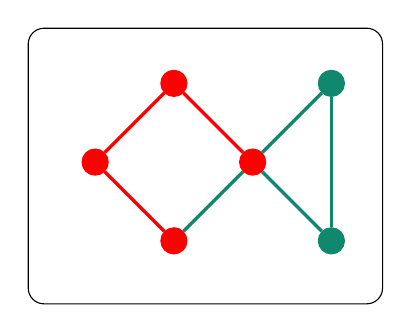
\begin{tikzpicture}
            \graphbox{}{0mm}{0mm}{45mm}{35mm}{-14mm}{-17mm}{
            \node[red,fill=red,draw, circle] (n1) at (0,0) {};
            \node[red,fill=red,draw, circle] (n2) at (1,1) {};
            \node[red,fill=red,draw, circle] (n3) at (2,0) {};
            \node[red,fill=red,draw, circle] (n4) at (1,-1) {};
            \node[PineGreen,fill=PineGreen,draw, circle] (n5) at (3,-1) {};
            \node[PineGreen,fill=PineGreen,draw, circle] (n6) at (3,1) {};
            \draw[very thick, red,-] (n1)-- node[pos=0.6, left] {} (n2);
            \draw[very thick, red,-] (n2)-- node[pos=0.35,right] {} (n3);
            \draw[very thick, PineGreen,-] (n3)-- node[pos=0.6,right] {}(n4);
            \draw[very thick, red,-] (n4)-- node[pos=0.45,left] {}(n1);
            \draw[very thick, PineGreen,-] (n3)-- node[pos=0.65,left] {}(n6);
            \draw[very thick, PineGreen,-] (n6)-- node[pos=0.4,right] {}(n5);
            \draw[very thick, PineGreen,-] (n5)-- node[pos=0.4,left] {}(n3);
            }
        \end{tikzpicture}
        \end{onlyenv}
         \begin{onlyenv}<8>
               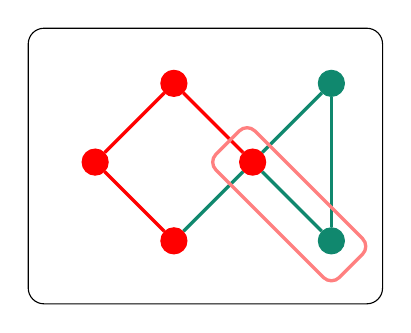
\begin{tikzpicture}
            \graphbox{}{0mm}{0mm}{45mm}{35mm}{-14mm}{-17mm}{
            \node[red,fill=red,draw, circle] (n1) at (0,0) {};
            \node[red,fill=red,draw, circle] (n2) at (1,1) {};
            \node[red,fill=red,draw, circle] (n3) at (2,0) {};
            \node[red,fill=red,draw, circle] (n4) at (1,-1) {};
            \node[PineGreen,fill=PineGreen,draw, circle] (n5) at (3,-1) {};
            \node[PineGreen,fill=PineGreen,draw, circle] (n6) at (3,1) {};
            \draw[very thick, red,-] (n1)-- node[pos=0.6, left] {} (n2);
            \draw[very thick, red,-] (n2)-- node[pos=0.35,right] {} (n3);
            \draw[very thick, PineGreen,-] (n3)-- node[pos=0.6,right] {}(n4);
            \draw[very thick, red,-] (n4)-- node[pos=0.45,left] {}(n1);
            \draw[very thick, PineGreen,-] (n3)-- node[pos=0.65,left] {}(n6);
            \draw[very thick, PineGreen,-] (n6)-- node[pos=0.4,right] {}(n5);
            \draw[very thick, PineGreen,-] (n5)-- node[pos=0.4,left] {}(n3);
            % \draw[red!50, rounded corners,rotate around={45:(1.5,0.5)}] ($(n3)+(-0.3,-0.3)$) rectangle ($(n6)+(0.3,0.3)$); 
            \draw[very thick, red!50, rounded corners,rotate around={45:(1.5,0.5)}] ($(n5)+(-0.4,-0.4)$) rectangle ($(n3)+(0.3,0.4)$); 
            }
        \end{tikzpicture}
        \end{onlyenv}
        \begin{onlyenv}<9>
            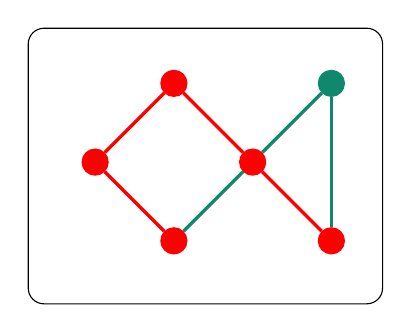
\begin{tikzpicture}
            \graphbox{}{0mm}{0mm}{45mm}{35mm}{-14mm}{-17mm}{
              \node[red,fill=red,draw, circle] (n1) at (0,0) {};
              \node[red,fill=red,draw, circle] (n2) at (1,1) {};
              \node[red,fill=red,draw, circle] (n3) at (2,0) {};
              \node[red,fill=red,draw, circle] (n4) at (1,-1) {};
              \node[red,fill=red,draw, circle] (n5) at (3,-1) {};
              \node[PineGreen,fill=PineGreen,draw, circle] (n6) at (3,1) {};
              \draw[very thick, red,-] (n1)-- node[pos=0.6, left] {} (n2);
              \draw[very thick, red,-] (n2)-- node[pos=0.35,right] {} (n3);
              \draw[very thick, PineGreen,-] (n3)-- node[pos=0.6,right] {}(n4);
              \draw[very thick, red,-] (n4)-- node[pos=0.45,left] {}(n1);
              \draw[very thick, PineGreen,-] (n3)-- node[pos=0.65,left] {}(n6);
              \draw[very thick, PineGreen,-] (n6)-- node[pos=0.4,right] {}(n5);
              \draw[very thick, red,-] (n5)-- node[pos=0.4,left] {}(n3);
              }
          \end{tikzpicture}
        \end{onlyenv}
         \begin{onlyenv}<10>
               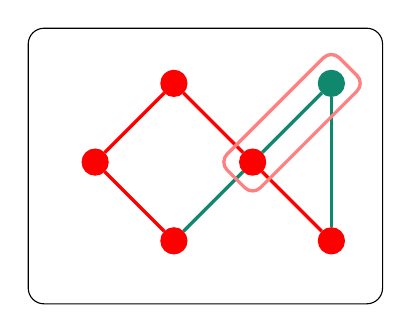
\begin{tikzpicture}
            \graphbox{}{0mm}{0mm}{45mm}{35mm}{-14mm}{-17mm}{
              \node[red,fill=red,draw, circle] (n1) at (0,0) {};
              \node[red,fill=red,draw, circle] (n2) at (1,1) {};
              \node[red,fill=red,draw, circle] (n3) at (2,0) {};
              \node[red,fill=red,draw, circle] (n4) at (1,-1) {};
              \node[red,fill=red,draw, circle] (n5) at (3,-1) {};
              \node[PineGreen,fill=PineGreen,draw, circle] (n6) at (3,1) {};
              \draw[very thick, red,-] (n1)-- node[pos=0.6, left] {} (n2);
              \draw[very thick, red,-] (n2)-- node[pos=0.35,right] {} (n3);
              \draw[very thick, PineGreen,-] (n3)-- node[pos=0.6,right] {}(n4);
              \draw[very thick, red,-] (n4)-- node[pos=0.45,left] {}(n1);
              \draw[very thick, PineGreen,-] (n3)-- node[pos=0.65,left] {}(n6);
              \draw[very thick, PineGreen,-] (n6)-- node[pos=0.4,right] {}(n5);
              \draw[very thick, red,-] (n5)-- node[pos=0.4,left] {}(n3);
              \draw[very thick, red!50, rounded corners,rotate around={45:(1.5,0.5)}] ($(n3)+(-0.3,-0.3)$) rectangle ($(n6)+(0.3,0.3)$); 
              % \draw[red!50, rounded corners,rotate around={45:(1.5,0.5)}] ($(n5)+(-0.4,-0.4)$) rectangle ($(n3)+(0.3,0.4)$); 
            }
        \end{tikzpicture}
        \end{onlyenv}
        \begin{onlyenv}<11>
               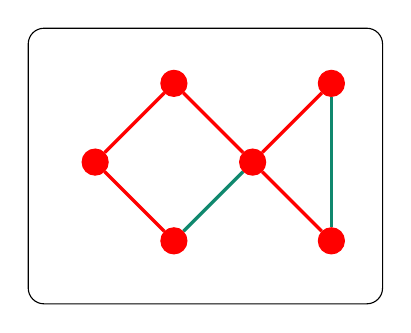
\begin{tikzpicture}
            \graphbox{}{0mm}{0mm}{45mm}{35mm}{-14mm}{-17mm}{
            \node[red,fill=red,draw, circle] (n1) at (0,0) {};
            \node[red,fill=red,draw, circle] (n2) at (1,1) {};
            \node[red,fill=red,draw, circle] (n3) at (2,0) {};
            \node[red,fill=red,draw, circle] (n4) at (1,-1) {};
            \node[red,fill=red,draw, circle] (n5) at (3,-1) {};
            \node[red,fill=red,draw, circle] (n6) at (3,1) {};
            \draw[very thick, red,-] (n1)-- node[pos=0.6, left] {} (n2);
            \draw[very thick, red,-] (n2)-- node[pos=0.35,right] {} (n3);
            \draw[very thick, PineGreen,-] (n3)-- node[pos=0.6,right] {}(n4);
            \draw[very thick, red,-] (n4)-- node[pos=0.45,left] {}(n1);
            \draw[very thick, red,-] (n3)-- node[pos=0.65,left] {}(n6);
            \draw[very thick, PineGreen,-] (n6)-- node[pos=0.4,right] {}(n5);
            \draw[very thick, red,-] (n5)-- node[pos=0.4,left] {}(n3);
            }
        \end{tikzpicture}
        \end{onlyenv}
          \begin{onlyenv}<12->
               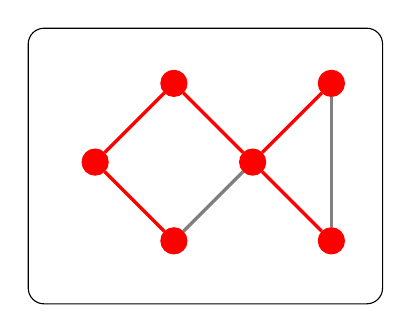
\begin{tikzpicture}
            \graphbox{}{0mm}{0mm}{45mm}{35mm}{-14mm}{-17mm}{
            \node[red,fill=red,draw, circle] (n1) at (0,0) {};
            \node[red,fill=red,draw, circle] (n2) at (1,1) {};
            \node[red,fill=red,draw, circle] (n3) at (2,0) {};
            \node[red,fill=red,draw, circle] (n4) at (1,-1) {};
            \node[red,fill=red,draw, circle] (n5) at (3,-1) {};
            \node[red,fill=red,draw, circle] (n6) at (3,1) {};
            \draw[very thick, red,-] (n1)-- node[pos=0.6, left] {} (n2);
            \draw[very thick, red,-] (n2)-- node[pos=0.35,right] {} (n3);
            \draw[very thick, gray,-] (n3)-- node[pos=0.6,right] {}(n4);
            \draw[very thick, red,-] (n4)-- node[pos=0.45,left] {}(n1);
            \draw[very thick, red,-] (n3)-- node[pos=0.65,left] {}(n6);
            \draw[very thick, gray,-] (n6)-- node[pos=0.4,right] {}(n5);
            \draw[very thick, red,-] (n5)-- node[pos=0.4,left] {}(n3);
            }
        \end{tikzpicture}
        \end{onlyenv}
     \end{center}

    \begin{onlyenv}<12->
          The result is a spanning tree.
    \end{onlyenv} 

        \begin{onlyenv}<13->
          \textcolor{red}{Does a result always exist?}
        \end{onlyenv} 
    \end{overlayarea}
    
\note{
L'exemple d'une règle de transformation de graphes est montré en haut.
Elle remplace une occurrence du graphe de gauche par celle de droite.

On peut appliquer cette règle pour construire un arbre couvrant du graphe en bas. 
À chaque étape, on recherche une occurrence du graphe de gauche dans le graphe courant, puis on la remplace par une occurrence du graphe de droite. 
Quand on ne peut plus appliquer la règle, les arêtes rouges du graphe resultant forment un arbre couvrant.

La question est de savoir si ce processus donne toujours un résultat, c'est-à-dire si la transformation se termine toujours.

1m30
}
\end{frame}


\begin{frame}{Graph Transformation: Termination}
  \begin{itemize}
    \item No graph $G_0$ can be transformed forever
         $$G_0 \Rightarrow G_1 \Rightarrow \cdots$$
        %  under the strategy 
        %   \begin{center}
        %       \textcolor{blue}{\enquote{apply rules as long as possible}}
        %   \end{center}
    \item Aligns with the notion of program termination: 
         \begin{center}
            \textcolor{blue}{\enquote{every execution (on any input) halts.}}
          \end{center}
    \item Undecidable in general
    %    \begin{itemize}
    %     \item Automated techniques for specific subclasses
    %    \end{itemize}
    \begin{itemize}
        \item Automated techniques
        \begin{itemize}
            \item \textcolor{red}{Power}: incomplete 
            \item \textcolor{red}{Usability}: rely on user-provided parameters
        \end{itemize}
    \end{itemize}
  \end{itemize}
    \note{
La terminaison d'un système de transformation de graphes signifie qu'il n'existe pas de graphe initial susceptible d'être transformé indéfiniment.

Cette notion coïncide avec la terminaison des programmes : chaque exécution sur n'importe quelle entrée s'arrête.

La terminaison des systèmes de transformation de graphes est indécidable en général, donc les techniques automatiques pour prouver la terminaison sont forcément incomplètes et reposent souvent sur des paramètres dépendant de l'intuition des utilisateurs.

1m
}
\end{frame}

\begin{frame}{Graph Transformation: A Non-Terminating Rule}
    \begin{center}
        \resizebox{0.8\textwidth}{!}{
    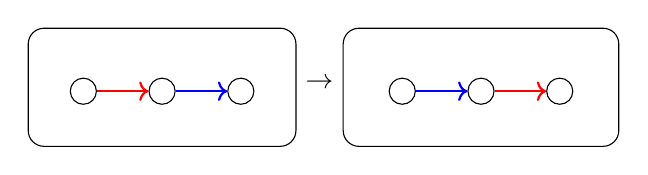
\begin{tikzpicture}[baseline=-10mm]
        \graphbox{}{0mm}{-3mm}{34mm}{15mm}{0mm}{3mm}{
            \coordinate (o) at (0mm,-11mm); 
            \node[draw,circle] (l1) at ($(o)+(-10mm,0mm)$) {};
            \node[draw,circle] (l2) at ($(l1)+(2,0)$) {};
            \node[draw,circle] (l3) at ($(l1)+(1,0)$) {};
            \draw[thick,->,red] (l1) -- (l3) node[midway,above] {};
            \draw[thick,->,blue] (l3) -- (l2) node[midway,above] {};
        } 

        \graphbox{}{40mm}{-3mm}{35mm}{15mm}{5mm}{3mm}{
            \coordinate (o) at (-5mm,-11mm); 
            \node[draw,circle] (l1) at ($(o)+(-10mm,0mm)$) {};
            % \node[draw,circle] (l2) at ($(l1)+(3,0)$) {2};
            \node[draw,circle] (l3) at ($(l1)+(1,0)$) {};
            \node[draw,circle] (l4) at ($(l1)+(2,0)$) {};
            \draw[thick,->,blue] (l1) -- (l3) node[midway,above] {};
            \draw[thick,->,red] (l3) -- (l4) node[midway,above] {};
            % \draw[->] (l4) -- (l2) node[midway,above] {$a$};
        }    
        % \node () at (37mm,-10mm) {\( \leftarrow \)}; % K -> L
        \node () at (37mm,-10mm) {\( \rightarrow \)}; % K -> R
    \end{tikzpicture}
    }
    \end{center}

\noindent Loop:\resizebox{0.85\textwidth}{!}{
    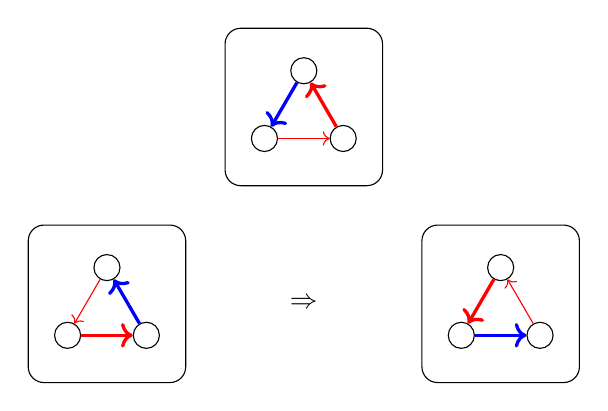
\begin{tikzpicture}[baseline=-10mm]
    \graphbox{\( \)}{0mm}{0mm}{20mm}{20mm}{-5mm}{-14mm}{
        \node[draw,circle] (x) at (0,0) {};
        \node[draw,circle] (y) at (1,0) {};
        \node[draw,circle] (z) at (0.5,0.86) {};
        \draw[->,red] (x) -- node[midway,below] {} (y) ;
        \draw[->,red,very thick] (y) -- node[midway,right] {} (z) ;
        \draw[->,blue,very thick] (z) -- node[midway,left] {} (x) ;
    } 
    \node () at (10mm,-35mm) {\( \Rightarrow  \)};
    \node () at (-3mm,-23mm) {\( \Swarrow  \)};
    \graphbox{\( \)}{-25mm}{-25mm}{20mm}{20mm}{-5mm}{-14mm}{
        \node[draw,circle] (x) at (0,0) {};  
        \node[draw,circle] (y) at (1,0) {};
        \node[draw,circle] (z) at (0.5,0.86) {};
        \draw[->,red,very thick] (x) -- node[midway,below] {} (y) ;
        \draw[->,blue,very thick] (y) -- node[midway,right] {} (z) ;
        \draw[->,red] (z) -- node[midway,left] {} (x) ;
    } 
    \node () at (23mm,-23mm) {\( \Nwarrow \)};
    \graphbox{\( \)}{25mm}{-25mm}{20mm}{20mm}{-5mm}{-14mm}{
        \node[draw,circle] (x) at (0,0) {};  
        \node[draw,circle] (y) at (1,0) {};
        \node[draw,circle] (z) at (0.5,0.86) {};
        \draw[->,blue,very thick] (x) -- node[midway,below] {} (y) ;
        \draw[->,red] (y) -- node[midway,right] {} (z) ;
        \draw[->,red,very thick] (z) -- node[midway,left] {} (x) ;
    }
    %   \node () at (85mm,-10mm) {\( \Rightarrow  \)};
    %   \graphbox{\( \)}{90mm}{0mm}{20mm}{20mm}{-5mm}{-14mm}{
    %       \node[draw,circle] (x) at (0,0) {};   
    %       \node[draw,circle] (y) at (1,0) {};
    %       \node[draw,circle] (z) at (0.5,0.86) {};
    %       \draw[->,red] (x) -- node[midway,below] {$a$} (y) ;
    %       \draw[->,red] (y) -- node[midway,right] {$b$} (z) ;
    %       \draw[->] (z) -- node[midway,left] {$b$} (x) ;
    %   }
    \end{tikzpicture}
    }

    \note{
        De nombreux travaux existent sur la terminaison des systèmes de réécriture de termes. En raison de différences structurelles — notamment la présence possible de circuits dans les graphes — ces méthodes ne s'appliquent pas directement aux systèmes de transformation de graphes.

        Voici un exemple simple d'une règle de transformation de graphes qui échange les couleurs de deux arêtes orientées. En appliquant cette règle au graphe en bas, on peut obtenir un cycle infini de transformations.
    }
\end{frame}

\begin{frame}{Graph Transformation: Termination by interpretations}
    \begin{beamercolorbox}[rounded=true,shadow=true,wd=\textwidth]{block body}
        \begin{description}
            \item[Interpret graphs as natural numbers.]
            \item[Show that each transformation step strictly decreases the value.]
        \end{description}
    \end{beamercolorbox}
\noindent   Number of edges: 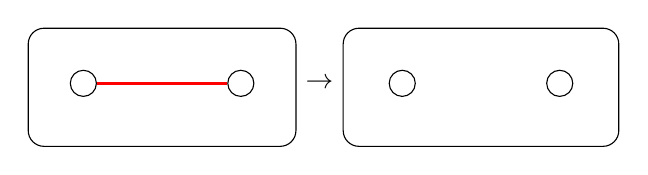
\begin{tikzpicture}[baseline=-12mm]
                    \graphbox{}{0mm}{-3mm}{34mm}{15mm}{0mm}{4mm}{
                        \coordinate (o) at (0mm,-11mm); 
                        \node[draw,circle] (l1) at ($(o)+(-10mm,0mm)$) {};
                        \node[draw,circle] (l2) at ($(l1)+(2,0)$) {};
                        \draw[very thick, red,-] (l1) -- (l2) node[midway,above] {};
                    } 
                    \graphbox{}{40mm}{-3mm}{35mm}{15mm}{5mm}{4mm}{
                        \coordinate (o) at (-5mm,-11mm); 
                        \node[draw,circle] (l1) at ($(o)+(-10mm,0mm)$) {};
                        \node[draw,circle] (l4) at ($(l1)+(2,0)$) {};
                    }    
                    \node () at (37mm,-10mm) {\( \rightarrow \)}; % K -> L
                \end{tikzpicture}
     \noindent  Number of nodes: 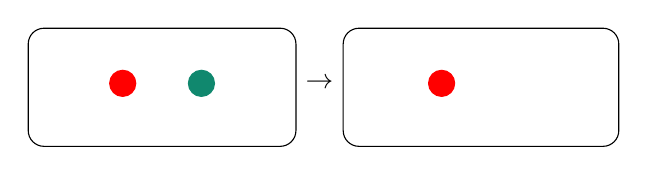
\begin{tikzpicture}[baseline=-12mm]
                    \graphbox{}{0mm}{-3mm}{34mm}{15mm}{0mm}{4mm}{
                        \coordinate (o) at (-5mm,-11mm); 
                        \node[fill=red,red,draw,circle] (l1) at ($(o)+(0mm,0mm)$) {};
                        \node[fill=PineGreen,PineGreen,draw,circle] (l3) at ($(l1)+(1,0)$) {};
                    }                     
                    \graphbox{}{40mm}{-3mm}{35mm}{15mm}{0mm}{4mm}{
                        \coordinate (o) at (-5mm,-11mm); 
                        \node[fill=red,red,draw,circle] (l1) at ($(o)+(0mm,0mm)$) {};
                    }    
                    \node () at (37mm,-10mm) {\( \rightarrow \)}; % K -> L
                \end{tikzpicture}

    \vspace{3mm}
      \noindent Number of edges labeled by $a$: 
    \begin{center}
       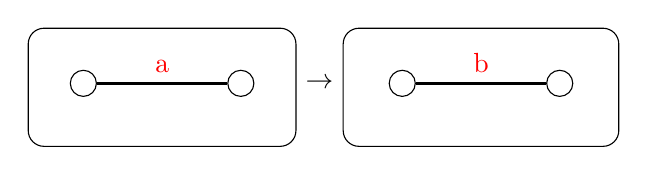
\begin{tikzpicture}
                    \graphbox{}{0mm}{-3mm}{34mm}{15mm}{0mm}{4mm}{
                        \coordinate (o) at (0mm,-11mm); 
                        \node[draw,circle] (l1) at ($(o)+(-10mm,0mm)$) {};
                        \node[draw,circle] (l2) at ($(l1)+(2,0)$) {};
                        \draw[very thick, -] (l1) -- (l2) node[midway,above] {\textcolor{red}{a}};
                    } 
                    \graphbox{}{40mm}{-3mm}{35mm}{15mm}{5mm}{4mm}{
                        \coordinate (o) at (-5mm,-11mm); 
                        \node[draw,circle] (l1) at ($(o)+(-10mm,0mm)$) {};
                        \node[draw,circle] (l4) at ($(l1)+(2,0)$) {};
                        \draw[very thick, -] (l1) -- (l4) node[midway,above] {\textcolor{red}{b}};
                    }    
                    \node () at (37mm,-10mm) {\( \rightarrow \)}; % K -> L
                \end{tikzpicture}
    \end{center}
   
    \note{
La terminaison peut être prouvée en associant aux graphes des valeurs entières, puis en montrant que chaque étape de transformation diminue strictement cette valeur.

Par exemple, la première règle diminue le nombre d'arêtes, 
la deuxième diminue le nombre de nœuds, 
et la troisième diminue le nombre d'arêtes étiquetées par a. 
Leur terminaison peut être prouvée 
en interprétant, respectivement, les graphes par le nombre d'arêtes, par le nombre de nœuds, et par le nombre d'arêtes étiquetées par a.

    1m
    }

\end{frame}

\begin{frame}{Limitations}
    \begin{center}
        \resizebox{\textwidth}{!}{ 
            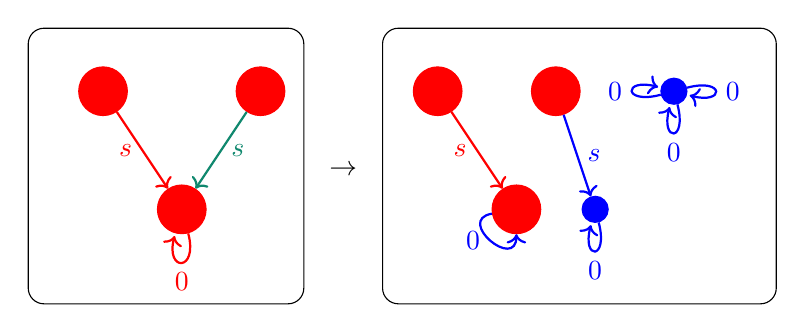
\begin{tikzpicture}
                \graphbox{}{0mm}{0mm}{35mm}{35mm}{2mm}{-5mm}{
                    \coordinate (delta) at (0,-18mm);
                    \node[red,fill=red,draw,circle] (l1) at ($(delta)+(-1,1.5)$) {1};
                    \node[red,fill=red,draw,circle] (l2) at ($(delta)+(1,1.5)$) {2};
                    \node[red,fill=red,draw,circle] (l3) at ($(delta)+(0,0)$) {3};
                    \draw[thick,red,->] (l1) -- (l3) node[midway,left] {$s$};
                    \draw[thick,PineGreen,->] (l2) -- (l3) node[midway,right] {$s$};
                    \draw[thick,red,->] (l3) edge [loop below] node {0} (l3);
                }
                    \node () at (40mm,-18mm) {$\rightarrow$};
                \graphbox{}{45mm}{0mm}{50mm}{35mm}{2mm}{-5mm}{
                    \coordinate (delta) at (-10mm,-18mm);
                    \node[red,fill=red,draw,circle] (r1) at ($(delta)+(-1,1.5)$) {1};
                    \node[red,fill=red,draw,circle] (r2) at ($(delta)+(0.5,1.5)$) {2};
                    \node[red,fill=red,draw,circle] (r3) at ($(delta)+(0,0)$) {3};
                    \node[blue,fill=blue,draw,circle] (r4) at ($(delta)+(1,0)$) {};
                    \draw[thick,red,fill=red,->] (r1) edge node[midway,left] {$s$} (r3) ;
                    \draw[thick,blue,->] (r2) -- (r4) node[midway,right] {$s$};
                    \draw[thick,blue,->] (r4) edge [loop below] node {0} (r4);
                    
                    \draw[thick,blue,->] (r3) edge [out=190,in=270,looseness=3] node[midway,left] {0} (r3);
                    \node[blue,fill=blue,draw,circle] (r5) at ($(r2)+(1.5,0)$) {};
                    \draw[thick,blue,->] (r5) edge [loop below] node {0} (r5);
                    \draw[thick,blue,->] (r5) edge [loop right] node {0} (r5);
                    \draw[thick,blue,->] (r5) edge [loop left] node {0} (r5);
                }
            \end{tikzpicture}
            }
    \end{center}

  \begin{itemize}
      \item The number of nodes/edges/labels does not decrease
    \item Can its termination be proved using interpretations?
  \end{itemize}
  \note{
Les interpretations naives présentées précédemment ne peuvent pas prouver la terminaison de cette règle, 
parce qu'elle ne diminue 
ni le nombre de nœuds, 
ni le nombre d'arêtes, 
ni le nombre d'arêtes avec une étiquette spécifique.

Peut-on trouver une interprétation pour prouver sa terminaison ?

30s
% 8s + 1m30 + 1m + 1m30 + 1m + 1m + 30s = 6m38s
  }

\end{frame}

\begin{frame}{}
    \tableofcontents
    \note{

    Nous présentons d'abord quelques notions de base, puis une définition formelle des transformations de graphes. 

    Ensuite, nous exposons une contribution qui améliore l'utilisabilité d'une méthode de terminaison, 

    puis notre contribution principale : une nouvelle technique de terminaison. 

    1m
    }
\end{frame}

\begin{frame}{Graph Morphisms: Structure-Preserving Functions}
             \begin{center}
          \resizebox{0.7\textwidth}{!}{
        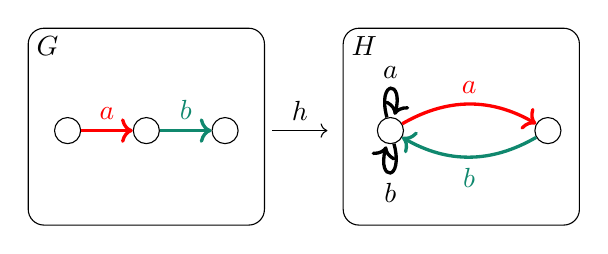
\begin{tikzpicture}
          \graphbox{$G$}{-40mm}{0mm}{30mm}{25mm}{0mm}{-3mm}{
            \coordinate (o) at (0mm,-10mm); 
            \node[draw,circle] (l1) at ($(o)+(-10mm,0mm)$) {};
            \node[draw,circle] (l2) at ($(l1)+(2,0)$) {};
            \node[draw,circle] (l3) at ($(l1)+(1,0)$) {};
            \draw[very thick, red,->] (l1) -- (l3) node[midway,above] {$a$};
            \draw[very thick, PineGreen,->] (l3) -- (l2) node[midway,above] {$b$};
        } 
            \graphbox{$H$}{0mm}{0mm}{30mm}{25mm}{-9mm}{-13mm}{
                \node[draw,circle] (1) at (0,0) {};
                \node[draw,circle] (2) at (2,0) {};
                \draw[very thick, ->] (1) edge[loop above] node[midway, above] {$a$} (1);
                \draw[very thick, ->] (1) edge[loop below] node[midway, below] {$b$} (1);
                \draw[very thick, ->,red] (1) edge[bend left] node[midway, above] {$a$}  (2);
                \draw[very thick, ->,PineGreen] (2) edge[bend left] node[midway, below] {$b$} (1);
            }
            % \node () at (-5mm,-15mm) {$\overset{h}{\to}$};
            \draw[->] (-9mm,-13mm) to node[midway,above] {$h$} (-2mm,-13mm);
        \end{tikzpicture}
          }
         \end{center}

    Colors indicate edge correspondence.
        \begin{center}
          \resizebox{0.7\textwidth}{!}{
        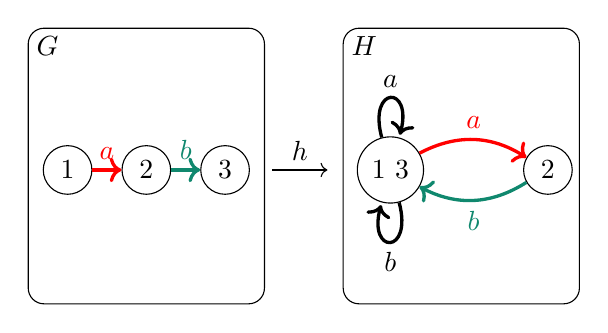
\begin{tikzpicture}
          \graphbox{$G$}{-40mm}{0mm}{30mm}{35mm}{0mm}{-8mm}{
            \coordinate (o) at (0mm,-10mm); 
            \node[draw,circle] (l1) at ($(o)+(-10mm,0mm)$) {1};
            \node[draw,circle] (l2) at ($(l1)+(2,0)$) {3};
            \node[draw,circle] (l3) at ($(l1)+(1,0)$) {2};
            \draw[very thick, red,->] (l1) -- (l3) node[midway,above] {$a$};
            \draw[very thick, PineGreen,->] (l3) -- (l2) node[midway,above] {$b$};
        } 
            \graphbox{$H$}{0mm}{0mm}{30mm}{35mm}{-9mm}{-18mm}{
                \node[draw,circle] (1) at (0,0) {1 3};
                \node[draw,circle] (2) at (2,0) {2};
                \draw[very thick, ->] (1) edge[loop above] node[midway, above] {$a$} (1);
                \draw[very thick, ->] (1) edge[loop below] node[midway, below] {$b$} (1);
                \draw[very thick, ->,red] (1) edge[bend left] node[midway, above] {$a$}  (2);
                \draw[very thick, ->,PineGreen] (2) edge[bend left] node[midway, below] {$b$} (1);
            }
            % \node () at (-5mm,-15mm) {$\overset{h}{\to}$};
            \draw[->] (-9mm,-18mm) to node[midway,above] {$h$} (-2mm,-18mm);
        \end{tikzpicture}
          }
         \end{center}

    Numbers indicate node correspondence.
    \note{
Un morphisme de graphes est une fonction qui envoie les nœuds et les arêtes d'un graphe vers ceux d'un autre en préservant la structure.

Nous utilisons des couleurs pour montrer la correspondance des arêtes 
et des numéros pour préciser la correspondance des nœuds, si necesaire.
    45s
    }
\end{frame}

\begin{frame}{Commutative Diagram}
      \begin{center}
                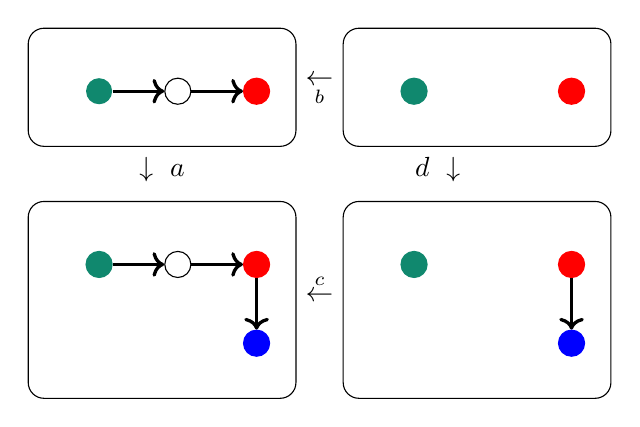
\begin{tikzpicture}
                    \graphbox{}{0mm}{0mm}{34mm}{15mm}{2mm}{0mm}{
                        \coordinate (o) at (0mm,-8mm); 
                        \node[PineGreen,fill=PineGreen,circle] (l1) at ($(o)+(-10mm,0mm)$) {};
                        \node[red,fill=red,draw,circle] (l2) at ($(l1)+(2,0)$) {};
                        \node[draw,circle] (l3) at ($(l1)+(1,0)$) {};
                        \draw[very thick, ->] (l1) -- (l3) node[midway,above] {};
                        \draw[very thick, ->] (l3) -- (l2) node[midway,above] {};
                    } 
                    \graphbox{}{40mm}{0mm}{34mm}{15mm}{2mm}{0mm}{
                        \coordinate (o) at (0mm,-8mm); 
                        \node[PineGreen,fill=PineGreen,draw,circle] (l1) at ($(o)+(-10mm,0mm)$) {};
                        \node[red,fill=red,draw,circle] (l2) at ($(l1)+(2,0)$) {};
                    }  
                
                    \graphbox{ }{0mm}{-22mm}{34mm}{25mm}{2mm}{-5mm}{
                        \coordinate (o) at (0mm,-3mm); 
                        \node[PineGreen,fill=PineGreen,draw,circle] (l1) at ($(o)+(-10mm,0mm)$) {};
                        \node[red,fill=red,draw,circle] (l2) at ($(l1)+(2,0)$) {};
                        \node[draw,circle ] (l3) at ($(l1)+(1,0)$) {};
                        \node[blue,fill=blue,draw,circle] (l4) at ($(l2)+(0,-1)$) {};
                        \draw[very thick, ->] (l1) -- (l3) node[midway,above] {};
                        \draw[very thick, ->] (l3) -- (l2) node[midway,above] {};
                        \draw[very thick, ->] (l2) -- (l4) node[midway,right] {};
                    }    
                    \graphbox{ }{40mm}{-22mm}{34mm}{25mm}{2mm}{-5mm}{
                        \coordinate (o) at (0mm,-3mm); 
                        \node[PineGreen,fill=PineGreen,draw,circle] (l1) at ($(o)+(-10mm,0mm)$) {};
                        \node[red,fill=red,draw,circle] (l2) at ($(l1)+(2,0)$) {};
                        \node[blue,fill=blue,draw,circle] (l4) at ($(l2)+(0,-1)$) {};
                        \draw[very thick, ->] (l2) -- (l4) node[midway,right] {};
                    }    
                    \node () at (37mm,-8mm) {\( \underset{b}{\leftarrow} \)};  
                    \node () at (17mm,-18mm) {\( \downarrow\ a \)};
                    \node () at (37mm,-33mm) {\( \overset{c}{\leftarrow} \)};
                    \node () at (52mm,-18mm) {\( d\ \downarrow \)};
            \end{tikzpicture}
        \end{center}
    \begin{beamercolorbox}[rounded=true,shadow=true,wd=\textwidth]{block body}
        \begin{center}
            \resizebox{0.3\textwidth}{!}{
                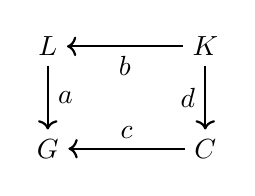
\begin{tikzpicture}
                    \node (I) at (0,-0.7) {$K$};
                    \node (L) at (-2,-0.7) {$L$};
                    \node (G) at (-2,-2) {$G$};
                    \node (C) at (0,-2) {$C$};
                    \draw [thick, ->] (I) to  node [midway,below] {$b$} (L);
                    \draw [thick, ->] (L) to node [midway,right] {$a$} (G);
                    \draw [thick, ->] (I) to node [midway,left] {$d$} (C);
                    \draw [thick, ->] (C) to node [midway,above] {$c$} (G);
                \end{tikzpicture}
            } 
        \end{center}
        commutes if \( a \circ b = c \circ d \).
    \end{beamercolorbox}
    \note{
    Considerons ce diagramme de morphismes de graphes.
    On dit qu'il commute parce que la composition des morphismes le long du chemin b puis a est égale à la composition le long du chemin d puis c.

    En général, on dit qu'un diagramme des morphismes commute si pour n'importe quel chemin entre deux graphes, la composition des morphismes le long de ce chemin est la même.

        45s
    }
\end{frame}

\begin{frame}{Pushouts: Gluing Graphs Along an Interface}
\begin{beamercolorbox}[rounded=true,shadow=true,wd=\textwidth]{block body}
    The \textbf{pushout} of \((\alpha,\beta) \)
    is  
        \( \textcolor{red}{(\beta',\alpha')}\) with
 
    \begin{itemize}
        \item $\square$\text{ABDC} commutes,
        \item<2->{universality:} \color{PineGreen}for all $(\gamma,\gamma')$,if $\square ABEC$ commutes, then there is a unique $\delta$ such that \text{$\triangle BDE$} and $\triangle CDE$ both commute.\color{black}
    \end{itemize} 
\end{beamercolorbox}
\begin{center}
    \begin{tikzpicture}[scale=0.8]
            \node (i) at (0,0) {A};
            \node (r) at (0,-2) {B};
            \node (c) at (2,0) {C};
            % \node () at (1,-1) {\( \Delta \)};
            \begin{onlyenv}<1->
                \draw[thick, ->]  (i) -- (r) node [pos=0.4,left] {$ \alpha $};
                \draw[thick, ->] (i) -- (c) node[pos=0.4, above] {$ \beta $};
            \end{onlyenv}
            \begin{onlyenv}<1->
                \node (h) at (2,-2) {\textcolor{red}{D}};
                \draw[thick, red,->] (c) -- (h) node [midway,left] {$ \alpha' $};
                \draw[thick, red,->] (r) -- (h) node[midway, above] {$ \beta' $};
                % \node () at ($(i)!.5!(h)$) {\textcolor{red}{PO}};
            \end{onlyenv}
            \begin{onlyenv}<2->
                \color{PineGreen}
                \node (d') at (3.5,-3.5) {E};
                \draw[thick, ->] (c) edge[bend left] node [midway,left]{$ \gamma' $} (d') ;
                \draw[thick, ->] (r) edge[bend right] node [midway,right]{$ \gamma $} (d') ;
                \draw[thick, ->,dashed] (h) -- (d') node [midway,above]{$ \delta $};
                \color{black}
            \end{onlyenv}
        \end{tikzpicture}
\end{center}
% $\square$ABDC: pushout square

D: pushout object
 \note{
    Le concept de pushout est essentiel dans la definition de la transformation de graphes que nous allons présenter.

    Le pushout d'un couple de morphismes \((\alpha,\beta) \) est un couple de morphismes \((\beta',\alpha')\) qui rend le diagramme ABDC commute et qui satisfait une propriété d'universalité.

    1m
 }
\end{frame}
\begin{frame}{Pushouts: Gluing Graphs Along an Interface}
    \begin{center}
        \resizebox{0.35\textwidth}{!}{
        \begin{tikzpicture}[scale=0.8]
                \node (i) at (0,0) {A};
                \node (r) at (0,-2) {B};
                \node (c) at (2,0) {C};
                % \node () at (1,-1) {\( \Delta \)};
                \begin{onlyenv}<1->
                    \draw[thick, ->]  (i) -- (r) node [pos=0.4,left] {$ \alpha $};
                    \draw[thick, ->] (i) -- (c) node[pos=0.4, above] {$ \beta $};
                \end{onlyenv}
                \begin{onlyenv}<1->
                    \node (h) at (2,-2) {\textcolor{red}{D}};
                    \draw[thick, red,->] (c) -- (h) node [midway,left] {$ \alpha' $};
                    \draw[thick, red,->] (r) -- (h) node[midway, above] {$ \beta' $};
                \end{onlyenv}
            \end{tikzpicture}
        }
        \hspace{0.1\textwidth}
        \resizebox{0.35\textwidth}{!}{
            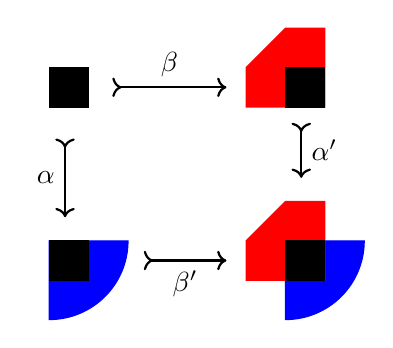
\begin{tikzpicture}  
                \coordinate (k) at (0, 0);
                \draw[black,fill=black] ($(k)+(0,0)$) rectangle ($(k)+(0.5,0.5)$);
                \coordinate (c) at (0, -2.2);
                \draw[fill=blue,blue]
                ($(c)+(0,-0.5)$)
                -- ($(c)+(0,0.5)$) 
                -- ($(c)+(1,0.5)$) 
                arc[start angle=0, end angle=-90, radius=1]
                -- cycle;
                \draw[black,fill=black] ($(c)+(0,0)$) rectangle ($(c)+(0.5,0.5)$);
        
                \coordinate (r) at (3,0);
                \draw[fill=red,red] ($(r)+(-0.5,0)$)
                -- ($(r)+(-0.5,0.5)$)
                -- ($(r)+(0,1)$)
                --  ($(r)+(0.5,1)$)
                -- ($(r)+(0.5,0)$)
                -- cycle;
                \draw[black,fill=black] ($(r)+(0,0)$) rectangle ($(r)+(0.5,0.5)$);
            
                \coordinate (h) at (3, -2.2);
                \draw[fill=blue,blue]
                ($(h)+(0,-0.5)$)
                -- ($(h)+(0,0.5)$)
                -- ($(h)+(1,0.5)$) 
                arc[start angle=0, end angle=-90, radius=1]
                -- cycle;
                \draw[fill=red,red] ($(h)+(-0.5,0)$)
                -- ($(h)+(-0.5,0.5)$)
                -- ($(h)+(0,1)$)
                --  ($(h)+(0.5,1)$)
                -- ($(h)+(0.5,0)$)
                -- cycle;
            \draw[black,fill=black] ($(h)+(0,0)$) rectangle ($(h)+(0.5,0.5)$);
                \draw[thick, >->] ($(k)!0.5!(r)+(-0.7,0.25)$)
                        -- node[midway,above] {$\beta$}  
                    ($(k)!0.5!(r)+(0.75,0.25)$);
                \draw[thick, >->]($(c)!0.5!(h)+(-0.3,0.25)$)
                        -- node[midway,below]  {$\beta'$}  
                    ($(c)!0.5!(h)+(0.75,0.25)$);
                
                    \draw[thick, <-<]($(k)!0.5!(c)+(0.2,-0.3)$)
                        -- node[midway,left]  {$\alpha$}  
                    ($(k)!0.5!(c)+(0.2,0.7)$);
                
                    \draw[thick, >->]($(r)!0.5!(h)+(0.2,0.9)$)
                        -- node[midway,right]  {$\alpha'$}  
                    ($(r)!0.5!(h)+(0.2,0.2)$);
            \end{tikzpicture}
        }
        \end{center}
       \begin{center}
        \resizebox{0.5\textwidth}{!}{
             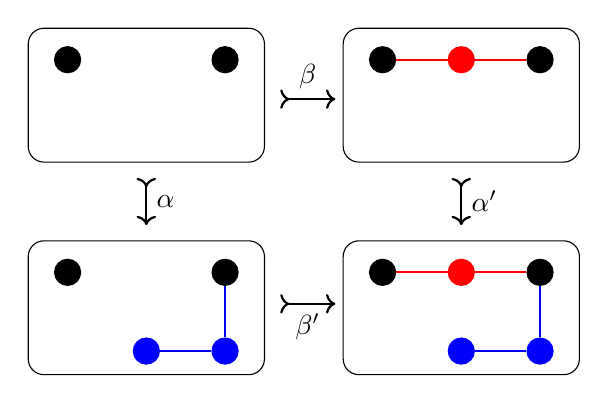
\begin{tikzpicture}
              \graphbox{}{0mm}{5mm}{30mm}{17mm}{2mm}{-5mm}{
                 \coordinate (o) at (-2mm,1mm); 
                  \node[black,fill=black,draw,circle] (l1) at ($(o)+(-10mm,0mm)$) {};
                  \node[black,fill=black,draw,circle] (l2) at ($(l1)+(2,0)$) {};
              } 

              \graphbox{}{40mm}{5mm}{30mm}{17mm}{2mm}{-5mm}{
                \coordinate (o) at (-2mm,1mm); 
                  \node[black,fill=black,draw,circle] (l1) at ($(o)+(-10mm,0mm)$) {};
                  \node[black,fill=black,draw,circle] (l2) at ($(l1)+(2,0)$) {};
                  \node[red,draw,circle,fill=red] (l3) at ($(l1)+(1,0)$) {};
                  \draw[thick, red] (l1) -- (l3) node[midway,above] {};
                  \draw[thick, red] (l3) -- (l2) node[midway,above] {};
              }  

              \graphbox{}{0mm}{-22mm}{30mm}{17mm}{2mm}{-5mm}{
                \coordinate (o) at (-2mm,1mm);
                  \node[black,fill=black,draw,circle] (l1) at ($(o)+(-10mm,0mm)$) {};
                  \node[black,fill=black,draw,circle] (l2) at ($(l1)+(2,0)$) {};
                  \node[blue,draw,circle,fill=blue] (l4) at ($(l2)+(0,-1)$) {};
                  \draw[thick, blue] (l2) -- (l4) node[midway,right] {};
                    \node[blue,draw,circle,fill=blue] (l7) at ($(l4)+(-1,0)$) {};
                  \draw[thick, blue] (l4) -- (l7) node[midway,below] {};
              }    

              \graphbox{}{40mm}{-22mm}{30mm}{17mm}{2mm}{-5mm}{
                \coordinate (o) at (-2mm,1mm);
                  \node[black,fill=black,draw,circle] (l1) at ($(o)+(-10mm,0mm)$) {};
                  \node[black,fill=black,draw,circle] (l2) at ($(l1)+(2,0)$) {};
                  \node[red,draw,circle,fill=red] (l3) at ($(l1)+(1,0)$) {};
                  \node[blue,draw,circle,fill=blue] (l4) at ($(l2)+(0,-1)$) {};
                  \draw[thick, red] (l1) -- (l3) node[midway,above] {};
                  \draw[thick, red] (l3) -- (l2) node[midway,above] {};
                  \draw[thick, blue] (l2) -- (l4) node[midway,right] {};
                \node[blue,draw,circle,fill=blue] (l7) at ($(l4)+(-1,0)$) {};
                  \draw[thick, blue] (l4) -- (l7) node[midway,below] {};
              }    

              \draw[thick, >->] (32mm,-4mm) to node[midway,above] {$\beta$} (39mm,-4mm);
              \draw[thick, >->] (15mm,-14mm) to node[midway,right] {$\alpha$} (15mm,-20mm);
              \draw[thick, >->] (32mm,-30mm) to node[midway,below] {$\beta'$} (39mm,-30mm);
              \draw[thick, >->] (55mm,-14mm) to node[midway,right] {$\alpha'$} (55mm,-20mm);
      \end{tikzpicture}
        }
    \end{center}
    \note{
        quand $\alpha$ et $\beta$ sont injectives, on peut voir les graphes B et C comme deux extensions de l'interface A.
        Et le pushout object D est obtenu en collant ensemble ces deux extensions via l'interface A.



        40s
    }
\end{frame}

\section{Formal Definition of Graph Rewriting}

\begin{frame}{Graph Rewriting with Double-Pushout (DPO)}
    \begin{description}
        \item[First algebraic approach]
        \item[One of the most studied approaches]  
    \end{description}
    \begin{overlayarea}{\textwidth}{\textheight}
    \begin{beamercolorbox}[rounded=true,shadow=true,wd=\textwidth]{block body}
        \resizebox{!}{0.25\textheight}{
            \begin{tikzpicture}
                \begin{onlyenv}<1->
                    \node (I) at (0,0) {$K$};
                    \node (L) at (-2,0) {$L$};
                    \node (R) at (2,0) {$R$};
                    \draw [thick, ->] (I) to  node [midway,above] {$l$} (L);
                    \draw [thick, ->] (I) to  node [midway,above] {$r$} (R);
                    \draw[fill=red,opacity=0.1 , rounded corners, dotted] (-2.5,-0.5) rectangle (2.5,0.5);
                    \node () at (5.5,0) {Rewriting rule with \textcolor{red}{interface $K$}};
                \end{onlyenv} 
                \begin{onlyenv}<2->
                    \node (G) at (-2,-1.5) {$G$};
                    \draw [thick, >->] (L) to node [midway,right] {} (G);
                \end{onlyenv}
                \begin{onlyenv}<3->
                    \node (C) at (0,-1.5) {$C$};
                    \draw [thick, ->] (I) to node [midway,right] { } (C);
                    \node [at=($(I)!.5!(G)$)] {\normalfont PO};
                    \draw [thick, ->] (C) to node [midway,above] { } (G);
                \end{onlyenv}
                \begin{onlyenv}<4->
                    \node (H) at (2,-1.5) {$H$};
                    \draw [thick, ->] (R) to node [midway,left] { } (H);
                    \draw [thick, ->] (C) to node [midway,above] { } (H);
                    \node [at=($(I)!.5!(H)$)] {\normalfont PO};
                    \draw[fill=PineGreen,opacity=0.1 , rounded corners, dotted] (-2.5,-2) rectangle (2.5,-1);
                    \node () at (5.5,-1.5) {\text{rewriting step $G \Rightarrow H$}};
                \end{onlyenv}
                \end{tikzpicture}
        }
    \end{beamercolorbox}
    \vspace{-0.07\textheight}
  \begin{center}
    \resizebox{\textwidth}{!}{
      \begin{tikzpicture}
            \begin{onlyenv}<1->
                 \graphbox{\( L \)}{0mm}{5mm}{34mm}{15mm}{2mm}{0mm}{
                  \coordinate (o) at (0mm,-8mm); 
                  \node[draw,circle] (l1) at ($(o)+(-10mm,0mm)$) {1};
                  \node[draw,circle] (l2) at ($(l1)+(2,0)$) {2};
                  \node[orange,draw,circle] (l3) at ($(l1)+(1,0)$) {3};
                  \draw[thick, orange,->] (l1) -- (l3) node[midway,above] {$a$};
                  \draw[thick, orange,->] (l3) -- (l2) node[midway,above] {$a$};
              } 

              \graphbox{\( K \)}{40mm}{5mm}{34mm}{15mm}{2mm}{0mm}{
                  \coordinate (o) at (0mm,-8mm); 
                  \node[thick, draw,circle] (l1) at ($(o)+(-10mm,0mm)$) {1};
                  \node[thick, draw,circle] (l2) at ($(l1)+(2,0)$) {2};
              }  

              \graphbox{\( R\)}{80mm}{5mm}{45mm}{15mm}{2mm}{0mm}{
                  \coordinate (o) at (-5mm,-8mm); 
                  \node[draw,circle] (l1) at ($(o)+(-10mm,0mm)$) {1};
                  \node[draw,circle] (l2) at ($(l1)+(3,0)$) {2};
                  \node[red,draw,circle] (l3) at ($(l1)+(1,0)$) {4};
                  \node[red,draw,circle] (l4) at ($(l1)+(2,0)$) {5};
                  \draw[thick, red,->] (l1) -- (l3) node[midway,above] {$a$};
                  \draw[thick, red,->] (l3) -- (l4) node[midway,above] {$b$};
                  \draw[thick, red,->] (l4) -- (l2) node[midway,above] {$a$};
              }    
              \node () at (37mm,-3mm) {\( \overset{l}{\leftarrow} \)}; 
              \node () at (77mm,-3mm) {\( \overset{r}{\rightarrow} \)}; 
            \end{onlyenv} 
            \begin{onlyenv}<2->
                \graphbox{\( G  \)}{0mm}{-17mm}{34mm}{25mm}{2mm}{-5mm}{
                  \coordinate (o) at (0mm,-3mm); 
                  \node[draw,circle] (l1) at ($(o)+(-10mm,0mm)$) {1};
                  \node[draw,circle] (l2) at ($(l1)+(2,0)$) {2};
                  \node[draw,circle,orange] (l3) at ($(l1)+(1,0)$) {3};
                  \node[blue, draw,circle] (l4) at ($(l2)+(0,-1)$) {6};
                  \draw[thick, orange,->] (l1) -- (l3) node[midway,above] {$a$};
                  \draw[thick, orange,->] (l3) -- (l2) node[midway,above] {$a$};
                  \draw[thick, blue,->] (l2) -- (l4) node[midway,right] {$a$};
              }   
              \node () at (17mm,-13mm) {\( \downarrowtail \)};
            \end{onlyenv}
            \begin{onlyenv}<3-> 
                \graphbox{\( C  \)}{40mm}{-17mm}{34mm}{25mm}{2mm}{-5mm}{
                  \coordinate (o) at (0mm,-3mm); 
                  \node[draw,circle] (l1) at ($(o)+(-10mm,0mm)$) {1};
                  \node[draw,circle] (l2) at ($(l1)+(2,0)$) {2};
                  \node[blue,draw,circle] (l4) at ($(l2)+(0,-1)$) {6};
                  \draw[thick, blue,->] (l2) -- (l4) node[midway,right] {$a$};
                 }   
                \node () at (37mm,-28mm) {\( \leftarrow \)};
                 \node () at (52mm,-13mm) {\( \downarrow \)};
                 \node () at (37mm,-15mm) {\text{PO}};
            \end{onlyenv}
            \begin{onlyenv}<4-> 
              \graphbox{\( H   \)}{80mm}{-17mm}{45mm}{25mm}{2mm}{-5mm}{
                  \coordinate (o) at (-5mm,-3mm); 
                  \node[draw,circle] (l1) at ($(o)+(-10mm,0mm)$) {1};
                  \node[draw,circle] (l2) at ($(l1)+(3,0)$) {2};
                  \node[draw,circle,red] (l3) at ($(l1)+(1,0)$) {4};
                  \node[draw,circle,red] (l4) at ($(l1)+(2,0)$) {5};
                  \node[blue,draw,circle] (l5) at ($(l2)+(0,-1)$) {6};
                  \draw[thick, red,->] (l1) -- (l3) node[midway,above] {$a$};
                  \draw[thick, red,->] (l3) -- (l4) node[midway,above] {$b$};
                  \draw[thick, red,->] (l4) -- (l2) node[midway,above] {$a$};
                  \draw[thick, blue,->] (l2) -- (l5) node[midway,right] {$a$};
              }    
              \node () at (92mm,-13mm) {\( \downarrow \)};
              \node () at (77mm,-28mm) {\( \rightarrow \)}; 
                 \node () at (77mm,-15mm) {\text{PO}};
            \end{onlyenv} 
            
      \end{tikzpicture}
      }
   \end{center}
\end{overlayarea}
\note{
    Enfin, nous presentons la notion centrale de cette presentation: la réécriture de graphes avec double pushout.
    
    Une regle de réécriture de graphes avec double pushout est un couple de morphismes l et r qui partent le meme graphe de depart K, appelé l'interface.

    Pour appliquer cette regle a un graphe G, on cherche un morphisme injectif de L vers G, appelé le match.

    Ensuite, on construit un diagram de pushout. 

    Le graphe C est obtenu en supprimant de G les elements qui sont dans L mais pas dans K. 

    Enfin, on construit un autre diagram de pushout.

    Le graphe H est obtenu en combinant C avec les elements de R via l'interface K.

    On obtient ainsi une étape de réécriture transformant de G vers H.

    70s

    keywords: notion centrale
}
\end{frame}

\begin{frame}{An Invalid Rewriting Step}
    % of the edge \textcolor{red}{$3 \overset{a}{\rightarrow} 6$} in $G$:
    \begin{center}
        \resizebox{\textwidth}{!}{
        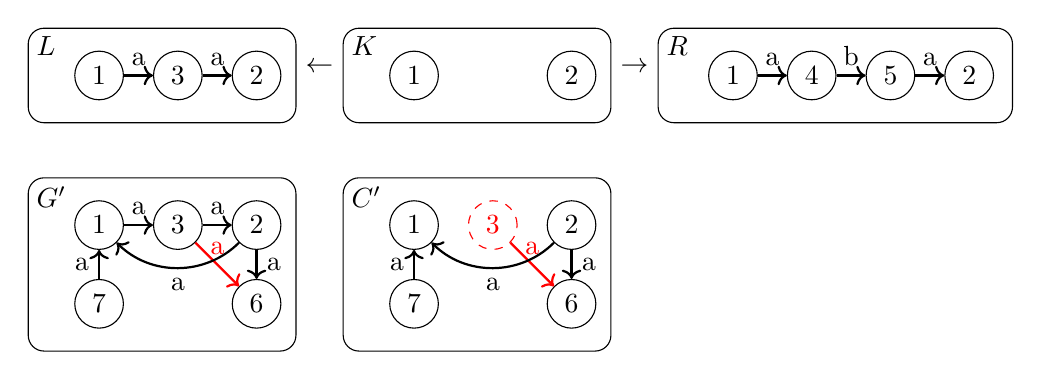
\begin{tikzpicture}
            \graphbox{\( L \)}{0mm}{-3mm}{34mm}{12mm}{2mm}{2mm}{
                \coordinate (o) at (0mm,-8mm); 
                \node[draw,circle] (l1) at ($(o)+(-10mm,0mm)$) {1};
                \node[draw,circle] (l2) at ($(l1)+(2,0)$) {2};
                \node[draw,circle] (l3) at ($(l1) + (1,0)$) {3};
                \draw[thick, ->] (l1) -- (l3) node[midway,above] {a};
                \draw[thick, ->] (l3) -- (l2) node[midway,above] {a};
            } 
    
            \graphbox{\( K \)}{40mm}{-3mm}{34mm}{12mm}{2mm}{2mm}{
                \coordinate (o) at (0mm,-8mm); 
                \node[draw,circle] (l1) at ($(o)+(-10mm,0mm)$) {1};
                \node[draw,circle] (l2) at ($(l1)+(2,0)$) {2};
            }  
    
            \graphbox{\( R \)}{80mm}{-3mm}{45mm}{12mm}{2mm}{2mm}{
                \coordinate (o) at (-5mm,-8mm); 
                \node[draw,circle] (l1) at ($(o)+(-10mm,0mm)$) {1};
                \node[draw,circle] (l2) at ($(l1)+(3,0)$) {2};
                \node[draw,circle] (l3) at ($(l1) + (1,0)$) {4};
                \node[draw,circle] (l4) at ($(l1) + (2,0)$) {5};
                \draw[thick, ->] (l1) -- (l3) node[midway,above] {a};
                \draw[thick, ->] (l3) -- (l4) node[midway,above] {b};
                \draw[thick, ->] (l4) -- (l2) node[midway,above] {a};
            }    
    
            \graphbox{\( G' \)}{0mm}{-22mm}{34mm}{22mm}{2mm}{-3mm}{
                \coordinate (o) at (0mm,-3mm); 
                \node[draw,circle] (l1) at ($(o)+(-10mm,0mm)$) {1};
                \node[draw,circle] (l2) at ($(l1)+(2,0)$) {2};
                \node[draw,circle] (l3) at ($(l1) + (1,0)$) {3};
                \node[draw,circle] (l4) at ($(l2) + (0,-1)$) {6};
                \draw[thick, ->,red] (l3) -- (l4) node[midway,above] {a};
                \draw[thick, ->] (l1) -- (l3) node[midway,above] {a};
                \draw[thick, ->] (l3) -- (l2) node[midway,above] {a};
                \draw[thick, ->] (l2) -- (l4) node[midway,right] {a};
                \node[draw,circle] (l6) at ($(l1) + (0,-1)$) {7};
                \draw[thick, <-] (l1) -- (l6) node[midway,left] {a};
                \draw[thick, ->] (l2) edge[out=-135,in=-45]node[midway,below] {a} (l1) ;
            }    
            % \onslide<2->{
                \graphbox{\( C'  \)}{40mm}{-22mm}{34mm}{22mm}{2mm}{-3mm}{
                    \coordinate (o) at (0mm,-3mm); 
                    \node[draw,circle] (l1) at ($(o)+(-10mm,0mm)$) {1};
                    \node[draw,circle] (l2) at ($(l1)+(2,0)$) {2};
                    \node[draw,circle] (l4) at ($(l2) + (0,-1)$) {6};
                    \node[draw,circle,dashed,red] (l3) at ($(l1) + (1,0)$) {3};
                    % \draw[->,red] (l3) -- (l4) node[midway,above] {a};
                    \draw[thick, ->,red] (l3) -- (l4) node[midway,above] {a};
                    \draw[thick, ->] (l2) -- (l4) node[midway,right] {a};
                    \draw[thick, ->] (l2) edge[out=-135,in=-45]node[midway,below] {a} (l1) ;
                    \node[draw,circle] (l6) at ($(l1) + (0,-1)$) {7};
                    \draw[thick, <-] (l1) -- (l6) node[midway,left] {a};
                }    
    
            % \graphbox{\( H' \)}{80mm}{-22mm}{45mm}{22mm}{2mm}{-3mm}{
            %     \coordinate (o) at (-5mm,-3mm); 
            %     \node[draw,circle] (l1) at ($(o)+(-10mm,0mm)$) {1};
            %     \node[draw,circle] (l2) at ($(l1)+(3,0)$) {2};
            %     \node[draw,circle] (l3) at ($(l1) + (1,0)$) {4};
            %     \node[draw,circle] (l4) at ($(l1) + (2,0)$) {5};
            %     \node[draw,circle] (l5) at ($(l2) + (0,-1)$) {6};
            %     \node[draw,circle] (l6) at ($(l1) + (0,-1)$) {7};
            %     \draw[<-] (l1) -- (l6) node[midway,left] {a};
            %     \draw[->] (l1) -- (l3) node[midway,above] {a};
            %     \draw[->] (l3) -- (l4) node[midway,above] {b};
            %     \draw[->] (l4) -- (l2) node[midway,above] {a};
            %     \draw[->] (l2) -- (l5) node[midway,right] {a};
            %     \draw[->] (l2) edge[out=-135,in=-45]node[midway,below] {a} (l1) ;
            %     \node[draw,circle,dashed,red] (l3) at (-0mm,-7mm) {3};
            %     \draw[->,red] (l3) -- (l5) node[midway,above] {a};
            % }    
    
            \node () at (37mm,-8mm) {\( \leftarrow \)}; % K -> L
            \node () at (77mm,-8mm) {\( \rightarrow \)}; % K -> R
            \node () at (15mm,-18mm) {\(\downarrowtail \)};
            % \node () at (37mm,-33mm) {\( \leftarrow \)};
            % \node () at (37mm,-18mm) {PO};
            % \node () at (58mm,-18mm) {\( \downarrow \)}; 
            % \node () at (80mm,-18mm) {PO};
            % \node () at (102mm,-18mm) {\( \downarrow \)};
            % \node () at (77mm,-33mm) {\( \rightarrow \)}; % C -> H
        \end{tikzpicture}
        }         
    \end{center}
    \textcolor{red}{No dangling edges should be created.}
    \note{

    Attention,
     on ne peut pas appliquer la règle avec ce match de L dans G' car la suppression du nœud 3 dans G' créerait une arête dans le vide.

    20s
    % 20s 70s 30s 40s 1m 45s 45s = 5m10s
    } 
\end{frame}

\section{Toward Greater Usability}

\begin{frame}{Weighted Type Graph Method}
Termination by interpretation
\newline\newline
Parameter: an object $T$ in the category, called the \textcolor{PineGreen}{type graph}.
\newline\newline
Terminology: every graph is \enquote{typed} by morphisms to $T$
\newline\newline
Interpretation:
\vspace{-3mm}
\begin{flalign*}
G &\leadsto \mathrm{morphisms}(G,T) \\
  &\leadsto \mathrm{weight}(\mathrm{morphisms}(G,T)) \\
  &\leadsto \mathrm{aggregator}(\mathrm{weight}(\mathrm{morphisms}(G,T)))\in\mathbb{N}
\end{flalign*}

% \only<2->{
\alert{
How to choose the type graph $T$?
\newline
How to define the morphism weight?
\newline
How to aggregate the morphism weights?
}
\note{
Une méthode très intéressante a été proposée par Bruggink et collegues en 2014, c'est la méthode par graphe de type pondéré.

Cette méthode a un paramètre (T), appelé le graphe de type.

Le nom vient du fait que chaque graphe (G) est considéré comme typé par l'ensemble des morphismes de (G) vers (T).

Un graphe (G) est d'abord interprété comme l'ensemble des morphismes de (G) vers (T). 

Ensuite, chaque morphisme est interprété comme un entier naturel. 

Enfin, les poids des morphismes sont agrégés pour obtenir un entier naturel.

La question est alors : comment choisir le graphe de type (T), 
comment définir le poids d'un morphisme, 
et comment agréger les poids des morphismes ?

Cette méthode a trois configurations possibles. 
Nous illustrerons l'une d'elles par un exemple 
afin d'éclairer les réponses aux deux dernières questions, 
puis nous présenterons la construction du graphe de type pondéré.

    90s
}
\end{frame}

\begin{frame}{Type Graph with Weights on Edges}
    \phantom{
        \begin{beamercolorbox}[rounded=true,shadow=true,wd=\textwidth]{block body}
        The weight of a morphism $h: G \rightarrow T$ is \[\sum_{e \in \opn{Edge(G)}}\mathrm{weight}(h(e)) \]
        \end{beamercolorbox}
    }
     \begin{center}
        \resizebox{\textwidth}{!}{
            \begin{tikzpicture}
              \phantom{
                \graphbox{\(L\)}{2mm}{0mm}{30mm}{20mm}{0mm}{0mm}{
                        \coordinate (o) at (0mm,-10mm); 
                        \node[draw,circle] (l1) at ($(o)+(-10mm,0mm)$) {};
                        \node[draw,circle] (l2) at ($(l1)+(2,0)$) {};
                        \node[draw,circle] (l3) at ($(l1)+(1,0)$) {};
                        \draw[->,red] (l1) -- (l3) node[midway,above] {$a$};
                        \draw[->,PineGreen] (l3) -- (l2) node[midway,above] {$b$};
                    } 
                  \graphbox{$T$}{-42mm}{10mm}{33mm}{40mm}{-8mm}{-20mm}{
                    \node[draw,circle] (1) at (0,0) {};
                    \node[draw,circle] (2) at (2,0) {};
                    \draw[->,red] (1) edge[loop above] node[midway, above] {$a^{1}$} (1) ;
                    \draw[->,PineGreen] (1) edge[loop below] node[midway, below] {$b^{0}$} (1) ;
                    \draw[->] (1) edge[bend left] node[midway, above] {$a^{0}$}  (2)  ;
                    \draw[->] (2) edge[bend left] node[midway, below] {$b^{0}$} (1) ;
                  }
                % \node () at (-3mm,-10mm) {$\overset{h_1}{\leftarrow}$};
                \draw[<-] (-7mm,-10mm) to node[midway,above] {$h_1$} (0mm,-10mm);
                 % \node () at (43mm,-10mm) {$\overset{h_2}{\to}$};
                    \draw[->] (34mm,-10mm) to node[midway,above] {$h_2$} (43mm,-10mm);
              }
            
                \graphbox{$T$}{45mm}{10mm}{35mm}{40mm}{-10mm}{-19mm}{
                    \node[draw,circle] (1) at (0,0) {};
                    \node[draw,circle] (2) at (2,0) {};
                    \draw[->] (1) edge[loop above] node[midway, above] {$a^{1}$} (1) ;
                    \draw[->] (1) edge[loop below] node[midway, below] {$b^{0}$} (1) ;
                    \draw[->,red] (1) edge[bend left] node[midway, above] {$a^{0}$}  (2)  ;
                    \draw[->,PineGreen] (2) edge[bend left] node[midway, below] {$b^{0}$} (1);
                }
                  
            \end{tikzpicture}
            }
    \end{center}
    \phantom{
            $ \mathrm{weight}_T(h) \mathop{=} \textcolor{red}{0} + \textcolor{PineGreen}{0} \mathop{=} 0$
        }

    \note{
        Nous fixons un graphe de type avec des poids sur les arêtes.


       10s
    }
\end{frame}
\begin{frame}{Morphism Weight}
     \begin{beamercolorbox}[rounded=true,shadow=true,wd=\textwidth]{block body}
      The weight of a morphism $h: G \rightarrow T$ is \[\sum_{e \in \opn{Edge(G)}}\mathrm{weight}(h(e)) \]
    \end{beamercolorbox}
    \begin{center}
        \resizebox{\textwidth}{!}{
            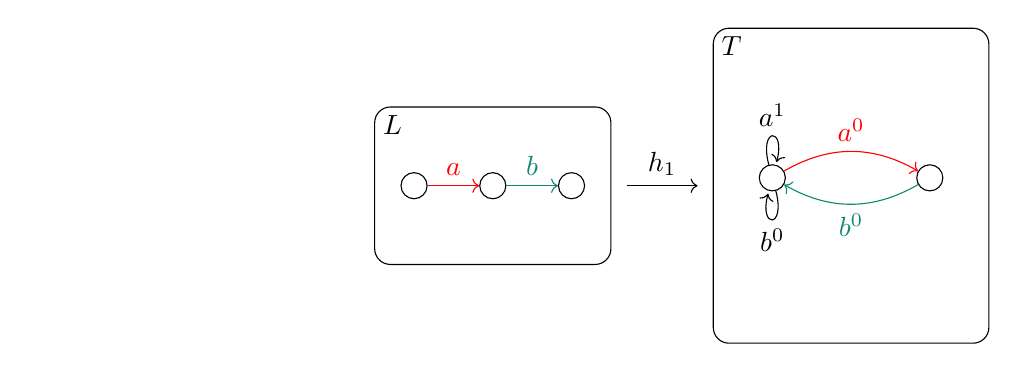
\begin{tikzpicture}
                \graphbox{\(L\)}{2mm}{0mm}{30mm}{20mm}{0mm}{0mm}{
                    \coordinate (o) at (0mm,-10mm); 
                    \node[draw,circle] (l1) at ($(o)+(-10mm,0mm)$) {};
                    \node[draw,circle] (l2) at ($(l1)+(2,0)$) {};
                    \node[draw,circle] (l3) at ($(l1)+(1,0)$) {};
                    \draw[->,red] (l1) -- (l3) node[midway,above] {$a$};
                    \draw[->,PineGreen] (l3) -- (l2) node[midway,above] {$b$};
                } 
              \phantom{
                  \graphbox{$T$}{-42mm}{10mm}{33mm}{40mm}{-8mm}{-20mm}{
                    \node[draw,circle] (1) at (0,0) {};
                    \node[draw,circle] (2) at (2,0) {};
                    \draw[->,red] (1) edge[loop above] node[midway, above] {$a^{1}$} (1) ;
                    \draw[->,PineGreen] (1) edge[loop below] node[midway, below] {$b^{0}$} (1) ;
                    \draw[->] (1) edge[bend left] node[midway, above] {$a^{0}$}  (2)  ;
                    \draw[->] (2) edge[bend left] node[midway, below] {$b^{0}$} (1) ;
                  }
                % \node () at (-3mm,-10mm) {$\overset{h_1}{\leftarrow}$};
                \draw[<-] (-7mm,-10mm) to node[midway,above] {$h_1$} (0mm,-10mm);
              }
            
                \graphbox{$T$}{45mm}{10mm}{35mm}{40mm}{-10mm}{-19mm}{
                    \node[draw,circle] (1) at (0,0) {};
                    \node[draw,circle] (2) at (2,0) {};
                    \draw[->] (1) edge[loop above] node[midway, above] {$a^{1}$} (1) ;
                    \draw[->] (1) edge[loop below] node[midway, below] {$b^{0}$} (1) ;
                    \draw[->,red] (1) edge[bend left] node[midway, above] {$a^{0}$}  (2)  ;
                    \draw[->,PineGreen] (2) edge[bend left] node[midway, below] {$b^{0}$} (1);
                }
                   % \node () at (43mm,-10mm) {$\overset{h_2}{\to}$};
                    \draw[->] (34mm,-10mm) to node[midway,above] {$h_1$} (43mm,-10mm);
            \end{tikzpicture}
            }
    \end{center}
    % \begin{center}
    % \resizebox{0.8\textwidth}{!}{
    %      \begin{tikzpicture}
    %       \graphbox{}{-50mm}{0mm}{40mm}{39mm}{2mm}{-6mm}{
    %         \coordinate (o) at (0mm,-10mm); 
    %         \node[draw,circle] (l1) at ($(o)+(-10mm,0mm)$) {};
    %         \node[draw,circle] (l2) at ($(l1)+(2,0)$) {};
    %         \node[draw,circle] (l3) at ($(l1)+(1,0)$) {};
    %         \draw[red,->] (l1) -- (l3) node[midway,above] {$a$};
    %         \draw[PineGreen,->] (l3) -- (l2) node[midway,above] {$b$};
    %     } 
    %     \draw[->] (-9mm,-17mm) to node[midway,above] {$h$} (-2mm,-17mm);
    %         \graphbox{$T$}{0mm}{0mm}{40mm}{39mm}{-12mm}{-19mm}{
    %             \node[draw,circle] (1) at (0,0) {};
    %             \node[draw,circle] (2) at (2,0) {};
    %             \draw[->] (1) edge[loop above] node[midway, above] {$a^{1}$} (1);
    %             \draw[->] (1) edge[loop below] node[midway, below] {$b^{0}$} (1);
    %             \draw[->,red] (1) edge[bend left] node[midway, above] {$a^{0}$}  (2);
    %             \draw[->,PineGreen] (2) edge[bend left] node[midway, below] {$b^{0}$} (1);
    %         }
    %     \end{tikzpicture}
    %     }
    % \end{center}
            \hspace{0.65\textwidth}$ \mathrm{weight}_T(h_1) \mathop{=} \textcolor{red}{0} + \textcolor{PineGreen}{0} \mathop{=} \textcolor{PineGreen}{0}$
    \note{
        Le poids du morphisme h1 est la somme des poids des images des arêtes de L.

        10s
    }
\end{frame}
 

\begin{frame}{Graph Weight} 
    \begin{beamercolorbox}[rounded=true,shadow=true,wd=\textwidth]{block body}
        The weight of a graph $L$ is \[\min \{h : L \mathop{\to} T \mid \mathrm{weight}_T(h)\}\]
    \end{beamercolorbox}
    \vspace{0.09\textheight}
    \begin{center}
        \resizebox{\textwidth}{!}{
            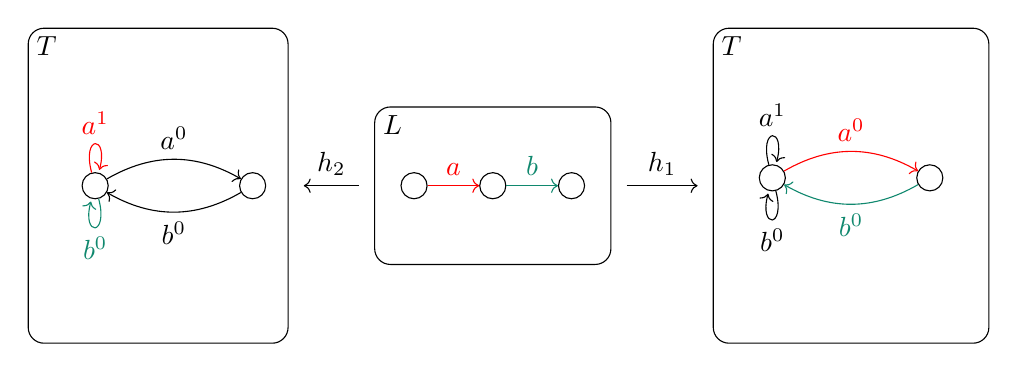
\begin{tikzpicture}
                \graphbox{\(L\)}{2mm}{0mm}{30mm}{20mm}{0mm}{0mm}{
                    \coordinate (o) at (0mm,-10mm); 
                    \node[draw,circle] (l1) at ($(o)+(-10mm,0mm)$) {};
                    \node[draw,circle] (l2) at ($(l1)+(2,0)$) {};
                    \node[draw,circle] (l3) at ($(l1)+(1,0)$) {};
                    \draw[->,red] (l1) -- (l3) node[midway,above] {$a$};
                    \draw[->,PineGreen] (l3) -- (l2) node[midway,above] {$b$};
                } 
                \graphbox{$T$}{-42mm}{10mm}{33mm}{40mm}{-8mm}{-20mm}{
                    \node[draw,circle] (1) at (0,0) {};
                    \node[draw,circle] (2) at (2,0) {};
                    \draw[->,red] (1) edge[loop above] node[midway, above] {$a^{1}$} (1) ;
                    \draw[->,PineGreen] (1) edge[loop below] node[midway, below] {$b^{0}$} (1) ;
                    \draw[->] (1) edge[bend left] node[midway, above] {$a^{0}$}  (2)  ;
                    \draw[->] (2) edge[bend left] node[midway, below] {$b^{0}$} (1) ;
                }
            
                \graphbox{$T$}{45mm}{10mm}{35mm}{40mm}{-10mm}{-19mm}{
                    \node[draw,circle] (1) at (0,0) {};
                    \node[draw,circle] (2) at (2,0) {};
                    \draw[->] (1) edge[loop above] node[midway, above] {$a^{1}$} (1) ;
                    \draw[->] (1) edge[loop below] node[midway, below] {$b^{0}$} (1) ;
                    \draw[->,red] (1) edge[bend left] node[midway, above] {$a^{0}$}  (2)  ;
                    \draw[->,PineGreen] (2) edge[bend left] node[midway, below] {$b^{0}$} (1);
                }
                % \node () at (43mm,-10mm) {$\overset{h_2}{\to}$};
                \draw[->] (34mm,-10mm) to node[midway,above] {$h_1$} (43mm,-10mm);
                % \node () at (-3mm,-10mm) {$\overset{h_1}{\leftarrow}$};
                \draw[<-] (-7mm,-10mm) to node[midway,above] {$h_2$} (0mm,-10mm);
            \end{tikzpicture}
            }
    \end{center}
    \begin{flalign*}
      & \mathrm{weight}_T(h_2) \mathop{=} \textcolor{red}{1} + \textcolor{PineGreen}{0} \mathop{=} \textcolor{red}{1} \hspace{0.1\textwidth} &\mathrm{weight}_T(h_1) \mathop{=} \textcolor{red}{0} + \textcolor{PineGreen}{0} \mathop{=} \textcolor{PineGreen}{0}\\
      &\mathrm{weight}_T(L) \mathop{=} \min \{\textcolor{red}{1}, \textcolor{PineGreen}{0}\} \mathop{=} 0 &
    \end{flalign*}
        % $\mathrm{weight}_T(L) \mathop{=} \min \{,\mathrm{weight}_T(h_2)\} = \min \{1+1, 1+0\}\mathop{=} 1$     
    \note{
        Le poids du graphe L est le poids minimal des morphismes de L vers T.

        Pour cet exemple, il y a deux morphismes, h1 et h2. 
        Le poids du morphisme h1 est 0, et le poids du morphisme h2 est 1.
        Donc, le poids de L est 0.

        40s
    }  
\end{frame}
   
\begin{frame}{Termination Criterion~[Bruggink \textit{et al.}, 2014]}
    %   \begin{beamercolorbox}[rounded=true,shadow=true,wd=\textwidth]{block body}
    \begin{center}
    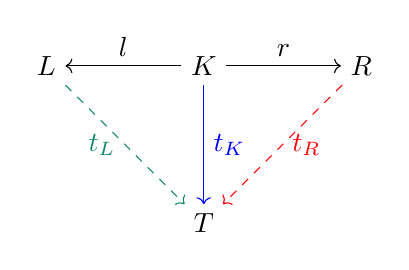
\begin{tikzpicture}
            \node (k) at (0,0) {$K$};
            \node (l) at (-2,0) {$L$};
            \node (t) at (0,-2) {$T$};
            \node (r) at (2,0) {$R$};
            \draw [->] (k) to  node [midway,above] {$l$} (l);
            \draw [->] (k) to  node [midway,above] {$r$} (r);
            \draw [->,blue] (k) to  node [midway,right] {\textcolor{blue}{$t_K$}} (t);
            \draw [->,dashed,PineGreen] (l) to node [midway,left] {\textcolor{PineGreen}{$t_L$}} (t);
            \draw [->,dashed,red] (r) to node [midway,right] {\textcolor{red}{$t_R$}} (t);
        \end{tikzpicture}
    \end{center}

      \begin{beamercolorbox}[rounded=true,shadow=true,wd=\textwidth]{block body}
        % Every rewriting step strictly decreases the weight
        A rule terminates \textcolor{red}{if there is a type graph $T$} such that for all \textcolor{blue}{$t_K$}, if there is \textcolor{PineGreen}{$t_L$} such that $\triangle KLT$ commutes, then 
        \begin{flalign*}
            &\min \{\opn{weight}_T(\textcolor{PineGreen}{t_L}) \mid t_L.\triangle KLT \text{commutes}\}  
            \\ \mathop{>}
            &\min \{\opn{weight}_T(\textcolor{red}{t_R}) \mid t_R.\triangle KRT \text{commutes}\}  
        \end{flalign*}
    \end{beamercolorbox}
 
   \alert{How to find a suitable weighted type graph?}
   \note{ 
        Selon une critère de terminaison proposé par Bruggink et collegues en 2014,

        Une règle de réécriture termine s'il existe un graphe de type T tel que pour tout morphisme tK de K vers T, 
        si il existe un morphisme tL de L vers T tel que le triangle KLT commute, 
        alors le poids minimal des morphismes tL tels que le triangle KLT commute est strictement supérieur au poids minimal des morphismes tR tels que le triangle KRT commute.

        La question est alors comment trouver un graphe de type pondéré approprié.
   }
\end{frame}

\begin{frame}{Searching for Weighted Type Graphs over $\mathbb{N}$}
    % Restricted search space:
    %   \begin{itemize}
    %     \item no parallel edges of the same label 
    %   \end{itemize}
    User-specified parameters:
      \begin{itemize}
        \item \textcolor{blue}{$k$ nodes}
        \item \textcolor{blue}{maximum edge weight $n\in\mathbb{N}$}
      \end{itemize}   
    The problem amounts to checking the satisfiability of an
\textcolor{blue}{existential Presburger arithmetic theory} with:
                \begin{itemize}
                  \item $k^2m$ binary variables where $m$ is the number of labels
                  \item $k^2m$ integer variables
                \end{itemize} 
  Challenges:
  \begin{itemize}
    \item \textcolor{red}{Usability}: difficult to guess $k$ and $n$
    \item \textcolor{red}{Search space}: $2^{k^2m} \cdot n^{k^2m}$ possible assignments of weights
  \end{itemize} 

  \note{ 
    Les travaux précédents suggerent de se restreindre à des graphes de type avec un nombre fixe de noeuds k et un poids maximum n. 

    Le problème revient à vérifier la satisfiabilité d'une théorie existentielle de l'arithmétique de Presburger avec des variables binaires et des variables entières.

    Le défi est double: d'une part, il est impossible pour l'utilisateur de deviner k et n.
    D'autre part, il y a un nombre important d'affectations des poids.

    1m
  }
\end{frame}

\begin{frame}{Usability Improvement}
    \textcolor{blue}{Idea:} Weights in $\mathbb{R}^{+}$

    \vspace{0.5cm}
    \textcolor{blue}{Additional constraint:} there is \textcolor{red}{$\delta > 0$} such that every rewriting step decreases the weight by at least \textcolor{red}{$\delta$}.
 
    \note{ 
        Afin d'améliorer l'utilisabilité de la méthode, 
        on propose d'utiliser des nombres réels positifs comme poids.
        
        Une contrainte supplementaire est tout fois nécessaire: il doit exister un delta strictement positif tel que chaque étape de réécriture diminue le poids d'au moins delta.

        30s
    }
\end{frame}

% \begin{frame}{Searching for Weighted Type Graphs over \crossout[red]{$\mathbb{N}$} $\mathbb{R}$}
%     User-specified parameters:
%       \begin{itemize}
%         \item \alert{$k$ nodes}
%         \item \crossout[red]{edge weights in $\{0, 1, \ldots, n\}$}
%       \end{itemize}   
%     % Assumption:
%     %   \begin{itemize}
%     %     \item no parallel edges of the same label 
%     %   \end{itemize}
%     The problem amounts to checking the satisfiability of an
% \crossout[red]{existential Presburger arithmetic theory} \textcolor{red}{existential theory of the reals with binary variables}:
%                 \begin{itemize}
%                   \item $k^2m$ binary variables where $m$ is the number of labels
%                   \item $k^2m$ \crossout[red]{integer} \textcolor{red}{real} variables
%                 \end{itemize} 
% %   Challenge:
% %   \begin{itemize}
% %     \item \crossout[red]{there are $2^{k^2m} \cdot n^{k^2m}$ possible assignments of weights}. \textcolor{red}{There are $2^{k^2m}$ linear programs which have polynomial-time average-case complexity.}
% %   \end{itemize} 
%     Challenge:
%   \begin{itemize}
%     \item impossible to guess $k$ and \crossout[red]{maximum weight $n$}
%     \item complexity: \crossout[red]{$2^{k^2m} \cdot n^{k^2m}$ possible assignments of weights} \textcolor{red}{there are $2^{k^2m}$ linear programs with $k^2m$ real variables, which have polynomial-time average-case complexity.}
%   \end{itemize} 
%     \note{ 
%         L'utilisateur n'a plus besoin de deviner le poids maximum.

%         Le problème revient à vérifier la satisfiabilité d'une théorie existentielle des réels avec des variables binaires et des variables réelles.

%         Il suffit de résoudre un nombre relativement petit de programmes linéaires avec peu de variables réelles. Ces programmes linéaires peuvent être résolus en temps polynomial en moyenne par rapport au nombre de variables par un solver.

%         1m
%     }
% \end{frame}


\begin{frame}{Searching for Weighted Type Graphs over \crossout[red]{$\mathbb{N}$} $\mathbb{R}$}
    User-specified parameters:
      \begin{itemize}
        \item \textcolor{blue}{$k$ nodes}
        \item \crossout[red]{\textcolor{blue}{edge weights in $\{0, 1, \ldots, n\}$}}
      \end{itemize}   
    % Assumption:
    %   \begin{itemize}
    %     \item no parallel edges of the same label 
    %   \end{itemize}
    The problem amounts to checking the satisfiability of an
\crossout[red]{\textcolor{blue}{existential Presburger arithmetic theory}} \textcolor{blue}{existential theory of the reals with binary variables}:
                \begin{itemize}
                  \item $k^2m$ binary variables where $m$ is the number of labels
                  \item $k^2m$ \crossout[red]{integer} \textcolor{blue}{real} variables
                \end{itemize} 
%   Challenge:
%   \begin{itemize}
%     \item \crossout[red]{there are $2^{k^2m} \cdot n^{k^2m}$ possible assignments of weights}. \textcolor{red}{There are $2^{k^2m}$ linear programs which have polynomial-time average-case complexity.}
%   \end{itemize} 
    Challenge:
  \begin{itemize}
    \item impossible to guess $k$ and \crossout[red]{maximum weight $n$}
    \item complexity: \crossout[red]{$2^{k^2m} \cdot n^{k^2m}$ possible assignments of weights} \textcolor{blue}{$2^{k^2m}$ linear programs which have polynomial-time average-case complexity.}
  \end{itemize} 

  \note{

        En utilisant des nombres réels positifs comme poids,

        L'utilisateur n'a plus besoin de deviner le poids maximum.
    
        Le problème revient à vérifier la satisfiabilité d'une théorie existentielle des réels avec des variables binaires et des variables réelles.
    
        Il suffit de résoudre un nombre relativement petit de programmes linéaires avec relativement peu de variables réelles. Ces programmes linéaires peuvent être résolus en temps polynomial en moyenne par rapport au nombre de variables par un solver.
    
        1m

  }

\end{frame}

\begin{frame}{Implementation$\leadsto$Experiments}
 $k$ from 1 to 4

 For every $k$, $n$ from 1 to 3 if over $\mathbb{N}$
    \begin{table}[htb]   
        \renewcommand{\arraystretch}{1.2}
        \centering
        \begin{adjustbox}{max width=\textwidth,max totalheight=0.8\textheight,keepaspectratio}
    \begin{tabular}{|c|H|c|H|c|H|c|}
        \hline
        &\;\;\text{Configuration 1}\;\;&\;\;\text{Configuration 1}\;\;&\;\;$T_{\mathbb{N}}$\;\;&\;\;\text{Configuration 2}\;\;&\;\; $N_{\mathbb{N}}$\;\;&\;\;\text{Configuration 3}\;\; \\
        \hline
    % ~\cite[Example 6.2]{endrullis2024generalized_arxiv_v2} & & & & & 2.68 &1.15   \\
    ~\cite[Example 6.3]{endrullis2024generalized_arxiv_v2} & & & & & 2.74 &\cellcolor{PineGreen}\textcolor{white}{58\%}
    % \textcolor{PineGreen}{1.16}  
     \\
        %~\cite[Example 6.4]{endrullis2024generalized_arxiv_v2}&  && & &  &   &  &  & our only Graph\\
    ~\cite[Example D.3]{endrullis2024generalized_arxiv_v2} &2.25 
        % (2.30+2.188+2.2637+2.2928+ 2.196) 
        &  
        \cellcolor{PineGreen}\textcolor{white}{48\%}
        % \textcolor{PineGreen}{1.18}
        % (1.17+1.2549+1.165+ 1.1576\mathop{+}1.162)
        & & & 2.24& \cellcolor{PineGreen}
        \textcolor{white}{47\%}
        % \textcolor{PineGreen}{1.18}   
         \\
    ~\cite[Example 3.8]{plump1995ontermination}
    & 2.95& 
    \cellcolor{PineGreen}\textcolor{white}{37\%} 
    %abs(2.95-1.90)/2.95=0.3559
    % \textcolor{PineGreen}{1.90} 
    & 2.94 &
        \cellcolor{PineGreen}\textcolor{white}{36\%} %abs(2.94-1.87)/2.94=0.3649
    % \cellcolor{PineGreen}\textcolor{PineGreen}{1.87}  
    & 3.49  &
    \textcolor{white}{36\%} %abs(3.49-1.87)/3.49=0.4639
    % \cellcolor{PineGreen}\textcolor{PineGreen}{1.87}   
    \\
        %~\cite[Example 3]{plump2018modular}
        % & 3.45& 3.44 & 3.55 &2.38  & 3.96  &17.60 &   4.24 AT &  3.45 at& 4.07 t  \\
    ~\cite[Example 4]{plump2018modular} &4.26
    & 
    \textcolor{white}{25\%}
    % \cellcolor{PineGreen}\textcolor{PineGreen}{3.19} 
    &  4.24 & 
    \textcolor{white}{26\%}
    \cellcolor{PineGreen}
    % \textcolor{PineGreen}{3.13} 
    &
        5.82
        % (5.77+5.83+5.775+5.84+5.818+5.89)
        & \cellcolor{blue}\textcolor{white}{timeout}  \\

    ~\cite[Example 5]{plump2018modular} & 5.54
        &\cellcolor{red}
        \textcolor{white}{1\%}
        % \textcolor{red}{5.55}
        % (5.53 +5.660\mathop{+}5.5213+5.5369+5.484689\mathop{+}5.6404\mathop{+}5.4877\mathop{+}5.5026)
        & 5.53& 
        \cellcolor{PineGreen}
        \textcolor{white}{1\%}
        % \textcolor{PineGreen}{5.50}
        & 9.11&  
        \cellcolor{PineGreen}
        \textcolor{white}{38\%}
        % \textcolor{PineGreen}{5.62}
          \\
    % ~\cite[Example 6]{plump2018modular} &  &  & & &  &   \\
        % (* en haut j'ai enverse tropical et arctic *)
        %~\cite[Example 6]{plump2018modular} &  &6.93 & 6.38 & 6.30 & 7.87&  7.22  &  11.71 at & 7.71 AT& 13.60 ATNat \\
    ~\cite[Example 4]{bruggink2015proving} &
        2.44
        % (2.4415+ 2.4181+2.4466+2.4366+2.4624+2.4479)
        & 
        \cellcolor{red}
        \textcolor{white}{1\%}
        % \textcolor{red}{2.46}
        % (2.4405+2.5180+2.4137+2.4539+2.4480+2.4750)
        & 
        2.47
        % (2.4660+2.4457+2.4559+2.4526+2.4588+2.4847+2.5731)/7
        &
        \cellcolor{red}
        \textcolor{white}{1\%}
        % \textcolor{red}{2.54}
        % (2.4380+2.4557+2.5590+2.5631+2.7245+2.5041+2.5182)/7
        & 4.58 & 
        \cellcolor{PineGreen}
        \textcolor{white}{46\%}
        % \textcolor{PineGreen}{2.46}
        % (2.3987+2.4521+2.4620+2.4558+2.5128+2.4507)/6
        \\
    ~\cite[Example 5]{bruggink2015proving} &  &  &&& 7.80& 
    \cellcolor{blue}
    \textcolor{white}{timeout} 
    \\
    ~\cite[Example 6]{bruggink2015proving} &  &  &&& 9.75& \cellcolor{blue}\textcolor{white}{timeout}   \\
    ~\cite[Example 1]{bruggink2014termination} & 
        2.26
        %  (2.2887\mathop{+}2.2386 +2.2719\mathop{+}2.2735 +2.3025\mathop{+}2.1925)/6
        &\cellcolor{PineGreen}
        \textcolor{white}{48\%}
        % \textcolor{PineGreen}{1.18}
        %  (1.1764+1.1837+1.1709+1.2222+1.1608+1.1645)/6
        & & &2.24
        %  (2.2365+2.2388+2.2124+2.2395+2.2550+2.2513)/6
        & \cellcolor{PineGreen}\textcolor{white}{47\%}
        % \textcolor{PineGreen}{1.18}  
        %  (1.2498+1.1710+1.1634+1.1655+1.1687+1.1733)/6
        \\
    ~\cite[Example 4]{bruggink2014termination} &  2.25
        % (2.2545+2.2512+2.2529+2.3498+2.2137+ 2.2257\mathop{+}2.2167\mathop{+}2.2413)/8
        & \cellcolor{PineGreen}
        \textcolor{white}{46\%}
        % \textcolor{PineGreen}{1.22} 
        & 2.24
        % (2.2981+2.2026\mathop{+}2.2229+2.2524+2.2421+2.2415)/6
        &\cellcolor{PineGreen}
        \textcolor{white}{47\%}
        % \textcolor{PineGreen}{1.18}
        % (1.1261+1.1850+1.1848+1.1706+1.2052+1.1920)/6
        &2.25
        % (2.2347+2.3106+2.2130+2.2391+2.2466+2.2493)/6 
        & \cellcolor{PineGreen}
        \textcolor{white}{49\%}
        % \textcolor{PineGreen}{1.19} 

        \\
    ~\cite[Example 5]{bruggink2014termination} &  4.23 
    & \cellcolor{PineGreen}
    \textcolor{white}{24\%}
    % \textcolor{PineGreen}{3.23}  
    & 4.25 &
    \cellcolor{PineGreen}
    \textcolor{white}{22\%}
    % \textcolor{PineGreen}{3.28}
    & 5.82 & \cellcolor{blue}\textcolor{white}{timeout} \\
         
        \hline
        \end{tabular}
    \end{adjustbox}
    \end{table}

 \resizebox{0.5\textwidth}{!}{\textbf{Usability Improved~\textcolor{PineGreen}{$\checkmark$}}}

    \note{ 
        On a implémenté la méthode par graphes de type pondérés dans un outil, et on a mené des expériences pour évaluer l'amélioration de la performance.
        
        Une case blanche indique que la configuration ne permet pas de prouver la terminaison.
        Une case en vert indique que l'utilisation de poids dans les réels est plus rapide, 
        une case en rouge indique que l'utilisation de poids dans les réels est plus lente,
        et une case en bleu indique que l'utilisation de poids dans les réels a entrainé un dépassement de temps, alors que l'utilisation de poids dans les entiers naturels a réussi en peu de temps.

        On remarque que pour les configurations 1 et 2, l'utilisation de poids dans les réels est systématiquement plus rapide.
        Pour la configuration 3, l'utilisation de poids dans les réels est plus rapide dans la majorité des cas, mais dans 4 cas, elle entraine un dépassement de temps. 
        Cela est dû au fait que la complexity est double exponentielle en le nombre de variables qui est trop élevé.
        Alors que dans les entiers naturels, meme si le probleme est undecidable, un graphe de type pondéré peut être trouvé rapidement en essayant l'ensemble des poids 0 et 1.

        1m     
    }
\end{frame}

\begin{frame}{A Limitation of the Weighted Type Graph Method}
     \begin{center}
        \resizebox{\textwidth}{!}{ 
            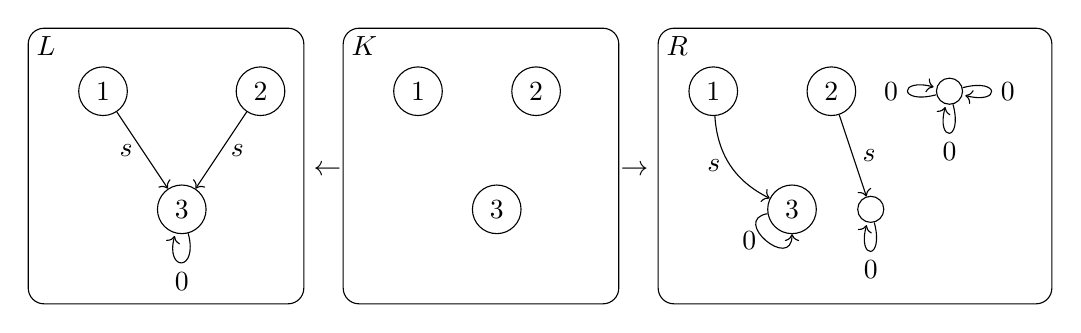
\begin{tikzpicture}
                \graphbox{$L$}{0mm}{0mm}{35mm}{35mm}{2mm}{-5mm}{
                    \coordinate (delta) at (0,-18mm);
                    \node[draw,circle] (l1) at ($(delta)+(-1,1.5)$) {1};
                    \node[draw,circle] (l2) at ($(delta)+(1,1.5)$) {2};
                    \node[draw,circle] (l3) at ($(delta)+(0,0)$) {3};
                    \draw[->] (l1) -- (l3) node[midway,left] {$s$};
                    \draw[->] (l2) -- (l3) node[midway,right] {$s$};
                    \draw[->] (l3) edge [loop below] node {0} (l3);
                }
                    \graphbox{$K$}{40mm}{0mm}{35mm}{35mm}{2mm}{-5mm}{
                        \coordinate (delta) at (0,-18mm);
                        \coordinate (interfaceorigin) at ($(delta) +(5,0)$);
                        \node[draw,circle] (r1) at ($(delta) +(-1,1.5)$) {1};
                        \node[draw,circle] (r2) at ($(delta) +(0.5,1.5)$) {2};
                        \node[draw,circle] (r3) at ($(delta)+(0,0)$) {3};
                    } 
                    \node () at (38mm,-18mm) {$\leftarrow$};
                    \node () at (77mm,-18mm) {$\rightarrow$};
                \graphbox{$R$}{80mm}{0mm}{50mm}{35mm}{2mm}{-5mm}{
                    \coordinate (delta) at (-10mm,-18mm);
                    \node[draw,circle] (r1) at ($(delta)+(-1,1.5)$) {1};
                    \node[draw,circle] (r2) at ($(delta)+(0.5,1.5)$) {2};
                    \node[draw,circle] (r3) at ($(delta)+(0,0)$) {3};
                    \node[draw,circle] (r4) at ($(delta)+(1,0)$) {};
                    \draw[->] (r1) edge[bend right] node[midway,left] {$s$} (r3) ;
                    \draw[->] (r2) -- (r4) node[midway,right] {$s$};
                    \draw[->] (r4) edge [loop below] node {0} (r4);
                    
                    \draw[->] (r3) edge [out=190,in=270,looseness=3] node[midway,left] {0} (r3);
                    \node[draw,circle] (r5) at ($(r2)+(1.5,0)$) {};
                    \draw[->] (r5) edge [loop below] node {0} (r5);
                    \draw[->] (r5) edge [loop right] node {0} (r5);
                    \draw[->] (r5) edge [loop left] node {0} (r5);
                }
            \end{tikzpicture}
            }
    \end{center}
Type graph fails: existence of surjections from $R$ to $L$

\textcolor{red}{All existing automated methods fail.}

 Remark: the number of occurrences of $\tikz[baseline=-0.5ex]{ 
                \node[draw,circle] (x) at (0,0) {}; 
                \node[draw,circle] (y) at (1,0) {};
                \node[draw,circle] (z) at (2,0) {};
                \draw[->] (x) -- (y) node[midway, above] {$s$};
                \draw[->] (z) -- (y) node[midway, above] {$s$};
    }$ strictly decreases.
 
 \note{
    On remarque cependant que la méthode par graphe de type pondéré a une limitation importante: elle ne peut pas prouver la terminaison d'une règle si il existe une surjection de R vers L, comme dans cet exemple.

    Pire encore, toutes les méthodes automatisées existantes échouent.

    On remarque que le nombre d'occurrences du graphe en bas diminue strictement.
    
    Ça suggère qu'une approche basée sur le comptage de sous-graphes pourrait être utile.
 }
\end{frame}

\section{Toward Greater Power}
% \begin{frame}
%   \tableofcontents[currentsection,hideothersubsections]
% \end{frame}

\begin{frame}{Capability Improvement: Morphism Counting}
    Parameter: graph $X$
    \newline\newline
    Interpretation:
        \vspace{-3mm}
        \begin{flalign*}
        G &\leadsto |\mathrm{morphisms}(X,G)| \in\mathbb{N}
        \end{flalign*}

    \note{
        On propose une nouvelle methode de termination par interpretation.

        Cette methode utilise un graphe X comme parametre.

        L'interpretation d'un graphe G est le nombre de morphismes de X vers G.

        Pour faciliter notre discussion, on va introduire d'abord une autre definition de reécriture de graphe après avoir présenté le concept d'inclusion. 
    }
\end{frame}

\begin{frame}{Inclusions}
         \begin{center} 
            \resizebox{\textwidth}{!}{
                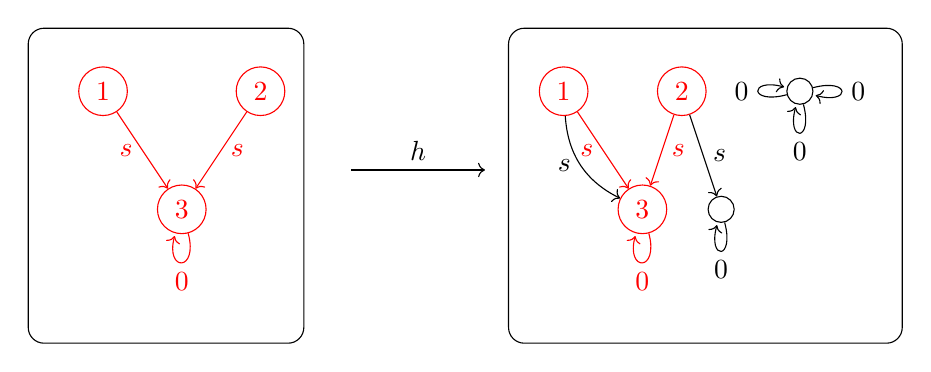
\begin{tikzpicture}
                    \graphbox{}{39mm}{0mm}{35mm}{40mm}{2mm}{-5mm}{
                        \coordinate (delta) at (0,-18mm);
                        \node[draw,circle,red] (l1) at ($(delta)+(-1,1.5)$) {1};
                        \node[draw,circle,red] (l2) at ($(delta)+(1,1.5)$) {2};
                        \node[draw,circle,red] (l3) at ($(delta)+(0,0)$) {3};
                        \draw[->,red] (l1) -- (l3) node[midway,left] {$s$};
                        \draw[->,red] (l2) -- (l3) node[midway,right] {$s$};
                        \draw[->,red] (l3) edge [loop below] node {0} (l3);
                    }
                        \draw[->] (80mm,-18mm) to node[midway,above] {$h$} (97mm,-18mm);
                    \graphbox{}{100mm}{0mm}{50mm}{40mm}{2mm}{-5mm}{
                        \coordinate (delta) at (-10mm,-18mm);
                        \node[draw,circle,red] (r1) at ($(delta)+(-1,1.5)$) {1};
                        \node[draw,circle,red] (r2) at ($(delta)+(0.5,1.5)$) {2};
                        \node[draw,circle,red] (r3) at ($(delta)+(0,0)$) {3};
                        \node[draw,circle] (r4) at ($(delta)+(1,0)$) {};
                        \node[draw,circle] (r5) at ($(r2)+(1.5,0)$) {};
                        \draw[->] (r1) edge[bend right] node[midway,left] {$s$} (r3) ; 
                        \draw[->] (r2) -- (r4) node[midway,right] {$s$};
                        \draw[->] (r4) edge [loop below] node {0} (r4);
                        \draw[->] (r5) edge [loop below] node {0} (r5);
                        \draw[->] (r5) edge [loop right] node {0} (r5);
                        \draw[->] (r5) edge [loop left] node {0} (r5);
                        \draw[->,red] (r1) edge node[midway,left] {$s$} (r3) ;
                        \draw[->,red] (r2) edge node[midway,right] {$s$} (r3) ; 
                        \draw[->,red] (r3) edge [loop below] node {0} (r3); 
                    }
                \end{tikzpicture}
                }
        \end{center}
 Subgraph
 \note{
 Avant de presenter la nouvelle méthode, je vais introduire le concept d'inclusion de graphe.
 
Une inclusion is a morphism whose domain is a subgraph of its codomain and every node and edge in the domain is mapped to itself in the codomain.
 }
 
\end{frame}
 
\begin{frame}{Graph Rewriting Systems}
  A rewriting rules consists of two inclusions. 
  \begin{center}
    $\varphi$=\resizebox{0.78\textwidth}{!}{
      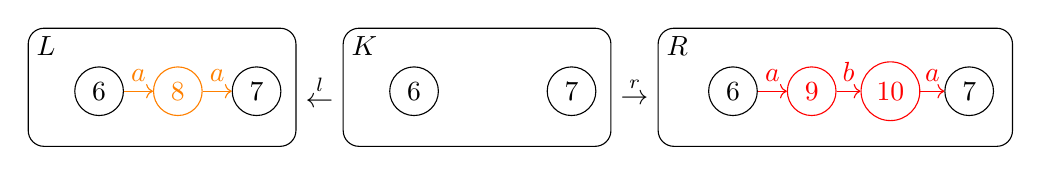
\begin{tikzpicture}[baseline=-10mm]
              \graphbox{\( L\)}{0mm}{5mm}{34mm}{15mm}{2mm}{0mm}{
                  \coordinate (o) at (0mm,-8mm); 
                  \node[draw,circle] (l1) at ($(o)+(-10mm,0mm)$) {6};
                  \node[draw,circle] (l2) at ($(l1)+(2,0)$) {7};
                  \node[orange,draw,circle] (l3) at ($(l1)+(1,0)$) {8};
                  \draw[orange,->] (l1) -- (l3) node[midway,above] {$a$};
                  \draw[orange,->] (l3) -- (l2) node[midway,above] {$a$};
              } 

              \graphbox{\( K \)}{40mm}{5mm}{34mm}{15mm}{2mm}{0mm}{
                  \coordinate (o) at (0mm,-8mm); 
                  \node[draw,circle] (l1) at ($(o)+(-10mm,0mm)$) {6};
                  \node[draw,circle] (l2) at ($(l1)+(2,0)$) {7};
              }  

              \graphbox{\( R \)}{80mm}{5mm}{45mm}{15mm}{2mm}{0mm}{
                  \coordinate (o) at (-5mm,-8mm); 
                  \node[draw,circle] (l1) at ($(o)+(-10mm,0mm)$) {6};
                  \node[draw,circle] (l2) at ($(l1)+(3,0)$) {7};
                  \node[red,draw,circle] (l3) at ($(l1)+(1,0)$) {9};
                  \node[red,draw,circle] (l4) at ($(l1)+(2,0)$) {10};
                  \draw[red,->] (l1) -- (l3) node[midway,above] {$a$};
                  \draw[red,->] (l3) -- (l4) node[midway,above] {$b$};
                  \draw[red,->] (l4) -- (l2) node[midway,above] {$a$};
              }    
              \node () at (37mm,-3mm) {\( \overset{l}{\leftarrow} \)}; % K -> L
              \node () at (77mm,-3mm) {\( \overset{r}{\rightarrow} \)}; % K -> R
      \end{tikzpicture}
      }
   \end{center}

   An equivalent rewriting rule expresses the same transformation. 

  \begin{center}
    $\varphi'$=\resizebox{0.78\textwidth}{!}{
      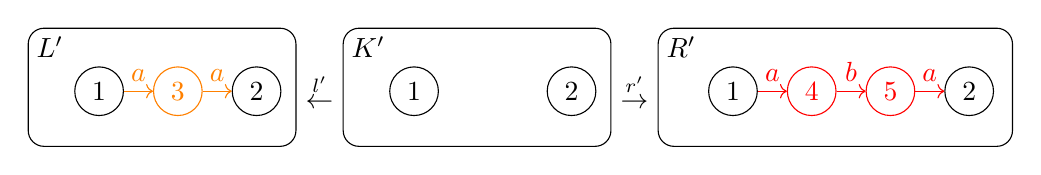
\begin{tikzpicture}[baseline=-10mm]
              \graphbox{\( L' \)}{0mm}{5mm}{34mm}{15mm}{2mm}{0mm}{
                  \coordinate (o) at (0mm,-8mm); 
                  \node[draw,circle] (l1) at ($(o)+(-10mm,0mm)$) {1};
                  \node[draw,circle] (l2) at ($(l1)+(2,0)$) {2};
                  \node[orange,draw,circle] (l3) at ($(l1)+(1,0)$) {3};
                  \draw[orange,->] (l1) -- (l3) node[midway,above] {$a$};
                  \draw[orange,->] (l3) -- (l2) node[midway,above] {$a$};
              } 

              \graphbox{\( K' \)}{40mm}{5mm}{34mm}{15mm}{2mm}{0mm}{
                  \coordinate (o) at (0mm,-8mm); 
                  \node[draw,circle] (l1) at ($(o)+(-10mm,0mm)$) {1};
                  \node[draw,circle] (l2) at ($(l1)+(2,0)$) {2};
              }  

              \graphbox{\( R' \)}{80mm}{5mm}{45mm}{15mm}{2mm}{0mm}{
                  \coordinate (o) at (-5mm,-8mm); 
                  \node[draw,circle] (l1) at ($(o)+(-10mm,0mm)$) {1};
                  \node[draw,circle] (l2) at ($(l1)+(3,0)$) {2};
                  \node[red,draw,circle] (l3) at ($(l1)+(1,0)$) {4};
                  \node[red,draw,circle] (l4) at ($(l1)+(2,0)$) {5};
                  \draw[red,->] (l1) -- (l3) node[midway,above] {$a$};
                  \draw[red,->] (l3) -- (l4) node[midway,above] {$b$};
                  \draw[red,->] (l4) -- (l2) node[midway,above] {$a$};
              }    
              \node () at (37mm,-3mm) {\( \overset{l'}{\leftarrow} \)}; 
              \node () at (77mm,-3mm) {\( \overset{r'}{\rightarrow} \)}; 
      \end{tikzpicture}
      }
   \end{center}
  
   A rewriting step with $\varphi$ is defined by a DPO diagram with inclusions and $\varphi'$.
  \begin{center}
    \resizebox{0.78\textwidth}{!}{
      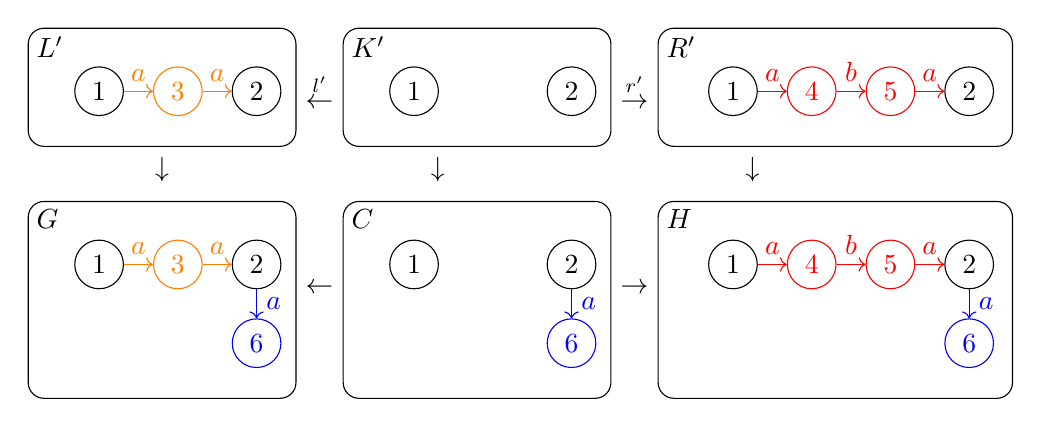
\begin{tikzpicture}
              \graphbox{\( L' \)}{0mm}{5mm}{34mm}{15mm}{2mm}{0mm}{
                  \coordinate (o) at (0mm,-8mm); 
                  \node[draw,circle] (l1) at ($(o)+(-10mm,0mm)$) {1};
                  \node[draw,circle] (l2) at ($(l1)+(2,0)$) {2};
                  \node[orange,draw,circle] (l3) at ($(l1)+(1,0)$) {3};
                  \draw[orange,->] (l1) -- (l3) node[midway,above] {$a$};
                  \draw[orange,->] (l3) -- (l2) node[midway,above] {$a$};
              } 

              \graphbox{\( K' \)}{40mm}{5mm}{34mm}{15mm}{2mm}{0mm}{
                  \coordinate (o) at (0mm,-8mm); 
                  \node[draw,circle] (l1) at ($(o)+(-10mm,0mm)$) {1};
                  \node[draw,circle] (l2) at ($(l1)+(2,0)$) {2};
              }  

              \graphbox{\( R' \)}{80mm}{5mm}{45mm}{15mm}{2mm}{0mm}{
                  \coordinate (o) at (-5mm,-8mm); 
                  \node[draw,circle] (l1) at ($(o)+(-10mm,0mm)$) {1};
                  \node[draw,circle] (l2) at ($(l1)+(3,0)$) {2};
                  \node[red,draw,circle] (l3) at ($(l1)+(1,0)$) {4};
                  \node[red,draw,circle] (l4) at ($(l1)+(2,0)$) {5};
                  \draw[red,->] (l1) -- (l3) node[midway,above] {$a$};
                  \draw[red,->] (l3) -- (l4) node[midway,above] {$b$};
                  \draw[red,->] (l4) -- (l2) node[midway,above] {$a$};
              }    
                \graphbox{\( G  \)}{0mm}{-17mm}{34mm}{25mm}{2mm}{-5mm}{
                  \coordinate (o) at (0mm,-3mm); 
                  \node[draw,circle] (l1) at ($(o)+(-10mm,0mm)$) {1};
                  \node[draw,circle] (l2) at ($(l1)+(2,0)$) {2};
                  \node[draw,circle,orange] (l3) at ($(l1)+(1,0)$) {3};
                  \node[blue, draw,circle] (l4) at ($(l2)+(0,-1)$) {6};
                  \draw[orange,->] (l1) -- (l3) node[midway,above] {$a$};
                  \draw[orange,->] (l3) -- (l2) node[midway,above] {$a$};
                  \draw[blue,->] (l2) -- (l4) node[midway,right] {$a$};
              }    
              \graphbox{\( C  \)}{40mm}{-17mm}{34mm}{25mm}{2mm}{-5mm}{
                  \coordinate (o) at (0mm,-3mm); 
                  \node[draw,circle] (l1) at ($(o)+(-10mm,0mm)$) {1};
                  \node[draw,circle] (l2) at ($(l1)+(2,0)$) {2};
                  \node[blue,draw,circle] (l4) at ($(l2)+(0,-1)$) {6};
                  \draw[blue,->] (l2) -- (l4) node[midway,right] {$a$};
              }    
              \graphbox{\( H   \)}{80mm}{-17mm}{45mm}{25mm}{2mm}{-5mm}{
                  \coordinate (o) at (-5mm,-3mm); 
                  \node[draw,circle] (l1) at ($(o)+(-10mm,0mm)$) {1};
                  \node[draw,circle] (l2) at ($(l1)+(3,0)$) {2};
                  \node[draw,circle,red] (l3) at ($(l1)+(1,0)$) {4};
                  \node[draw,circle,red] (l4) at ($(l1)+(2,0)$) {5};
                  \node[blue,draw,circle] (l5) at ($(l2)+(0,-1)$) {6};
                  \draw[red,->] (l1) -- (l3) node[midway,above] {$a$};
                  \draw[red,->] (l3) -- (l4) node[midway,above] {$b$};
                  \draw[red,->] (l4) -- (l2) node[midway,above] {$a$};
                  \draw[blue,->] (l2) -- (l5) node[midway,right] {$a$};
              }    
              \node () at (37mm,-3mm) {\( \overset{l'}{\leftarrow} \)}; 
              \node () at (77mm,-3mm) {\( \overset{r'}{\rightarrow} \)}; 
              \node () at (17mm,-13mm) {\( \downarrow \)};
              \node () at (37mm,-28mm) {\( \leftarrow \)};
              \node () at (52mm,-13mm) {\( \downarrow \)};
              \node () at (92mm,-13mm) {\( \downarrow \)};
              \node () at (77mm,-28mm) {\( \rightarrow \)};  
      \end{tikzpicture}
      }
   \end{center}
   \note{
    Une règle de reécriture de graphes consiste en deux inclusions.

    Deux règles sont équivalentes si elles expriment la même transformation.

    Une étape de reécriture avec une règle est définie par un diagramme de double pushout avec des inclusions et une règle équivalente en haut. 

    Afin de faciliter la discussion, on va introduire le concept de pré-graphe.
   }
\end{frame}

\begin{frame}{Pre-Graphs}
  \noindent Graph:
         \begin{center}
            \resizebox{0.5\textwidth}{!}{
            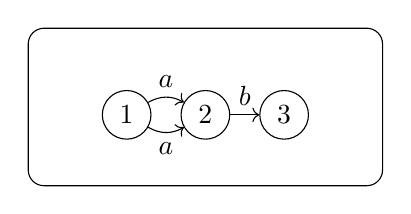
\begin{tikzpicture}
                \graphbox{}{0mm}{-20mm}{45mm}{20mm}{5mm}{-3mm}{ 
                    \coordinate (o) at (-5mm,-8mm); 
                    \node[draw,circle] (l1) at ($(o)+(-10mm,0mm)$) {1};
                    \node[draw,circle] (l3) at ($(l1)+(1,0)$) {2};
                    \node[draw,circle] (l4) at ($(l1)+(2,0)$) {3};
                    \draw[->] (l1) edge[bend right]  node[midway,below] {$a$} (l3);
                    \draw[->] (l1) edge[bend left] node[midway,above] {$a$}  (l3);
                    \draw[->] (l3) -- (l4) node[midway,above] {$b$};
                }  
            \end{tikzpicture} 
        }
        \end{center} 
    \begin{beamercolorbox}[rounded=true,shadow=true,wd=\textwidth]{block body}
    \noindent Pre-graphs obtained by removing node 2:
    \end{beamercolorbox}
        \begin{center}
            \resizebox{0.5\textwidth}{!}{
            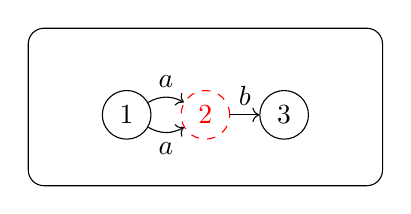
\begin{tikzpicture}
                \graphbox{}{0mm}{-20mm}{45mm}{20mm}{5mm}{-3mm}{ 
                    \coordinate (o) at (-5mm,-8mm); 
                    \node[draw,circle] (l1) at ($(o)+(-10mm,0mm)$) {1};
                    \node[draw,circle,dashed,red] (l3) at ($(l1)+(1,0)$) {2};
                    \node[draw,circle] (l4) at ($(l1)+(2,0)$) {3};
                    \draw[->] (l1) edge[bend right]  node[midway,below] {$a$} (l3);
                    \draw[->] (l1) edge[bend left] node[midway,above] {$a$}  (l3);
                    \draw[->] (l3) -- (l4) node[midway,above] {$b$};
                }  
            \end{tikzpicture} 
        }
        \end{center} 
Dangling edges
 \note{
    On appelle prégraphe un graphe dans lequel certaines arêtes peuvent être pendantes.

Par exemple, en supprimant le nœud 2 du graphe en haut, on obtient le prégraphe en bas présentant des arêtes pendantes.
 }
\end{frame}

\begin{frame}{Decomposition of Graphs in Rewriting Rules}
    \begin{center}
    \resizebox{0.85\textwidth}{!}{
      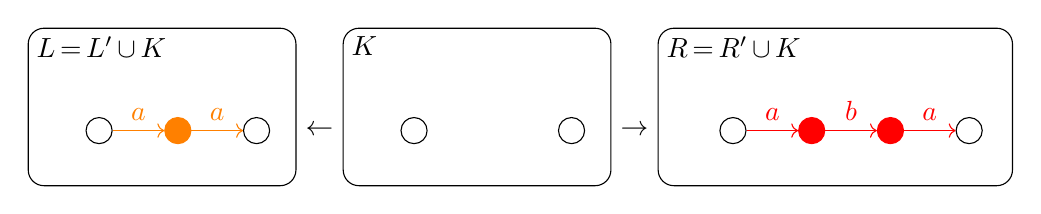
\begin{tikzpicture}
              \graphbox{\( L \mathop{=} L' \mathop{\cup} K \)}{0mm}{5mm}{34mm}{20mm}{2mm}{-5mm}{
                  \coordinate (o) at (0mm,-8mm); 
                  \node[draw,circle] (l1) at ($(o)+(-10mm,0mm)$) {};
                  \node[draw,circle] (l2) at ($(l1)+(2,0)$) {};
                  \node[orange,fill=orange,draw,circle] (l3) at ($(l1)+(1,0)$) {};
                  \draw[orange,fill=orange,->] (l1) -- (l3) node[midway,above] {$a$};
                  \draw[orange,fill=orange,->] (l3) -- (l2) node[midway,above] {$a$};
              } 

              \graphbox{\( K \)}{40mm}{5mm}{34mm}{20mm}{2mm}{-5mm}{
                  \coordinate (o) at (0mm,-8mm); 
                  \node[draw,circle] (l1) at ($(o)+(-10mm,0mm)$) {};
                  \node[draw,circle] (l2) at ($(l1)+(2,0)$) {};
              }  

              \graphbox{\( R \mathop{=} R' \mathop{\cup} K \)}{80mm}{5mm}{45mm}{20mm}{2mm}{-5mm}{
                  \coordinate (o) at (-5mm,-8mm); 
                  \node[draw,circle] (l1) at ($(o)+(-10mm,0mm)$) {};
                  \node[draw,circle] (l2) at ($(l1)+(3,0)$) {};
                  \node[red,fill=red,draw,circle] (l3) at ($(l1)+(1,0)$) {};
                  \node[red,fill=red,draw,circle] (l4) at ($(l1)+(2,0)$) {};
                  \draw[red,fill=red,->] (l1) -- (l3) node[midway,above] {$a$};
                  \draw[red,fill=red,->] (l3) -- (l4) node[midway,above] {$b$};
                  \draw[red,fill=red,->] (l4) -- (l2) node[midway,above] {$a$};
              }    

              \node () at (37mm,-8mm) {\( \leftarrow \)}; % K -> L
              \node () at (77mm,-8mm) {\( \rightarrow \)}; % K -> R
      \end{tikzpicture}
      }
   \end{center}
\begin{center}
    \resizebox{0.85\textwidth}{!}{
            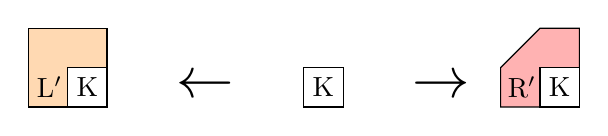
\begin{tikzpicture} 
                \coordinate (k) at (0, 0);
                \draw[fill=white] ($(k)+(0,0)$) rectangle ($(k)+(0.5,0.5)$);
                \node () at ($(k)+(0.25,0.25)$) {\( \mathrm{K} \)};
            
                \coordinate (l) at (-3, 0);
                \draw[fill=orange!30] ($(l)+(-0.5,0)$) rectangle ($(l)+(0.5,1)$);
                \node () at ($(l)+(-0.23,0.25)$) {\( \mathrm{L'} \)};
                \draw[fill=white] ($(l)+(0,0)$) rectangle ($(l)+(0.5,0.5)$);
                \node () at ($(l)+(0.25,0.25)$) {\( \mathrm{K} \)};
             
                \coordinate (r) at (3,0);
                \draw[fill=red!30] ($(r)+(-0.5,0)$)
                -- ($(r)+(-0.5,0.5)$)
                -- ($(r)+(0,1)$)
                --  ($(r)+(0.5,1)$)
                -- ($(r)+(0.5,0)$)
                -- cycle;
                \node () at ($(r)+(-0.23,0.25)$) {\( \mathrm{R'} \)};
                \draw[fill=white] ($(r)+(0,0)$) rectangle ($(r)+(0.5,0.5)$);
                \node () at ($(r)+(0.25,0.25)$) {\( \mathrm{K} \)};
             
                \node[ font=\huge] (kl) at ($(k)!0.5!(l)+(0.25,0.25)$)
                {\( \leftarrow \)}
                ; 
                \node[ font=\huge] (kr) at ($(k)!0.5!(r)+(0.25,0.25)$)
                {\( \rightarrow \)}
                ;  
            \end{tikzpicture}
          }
   \end{center}
   \note{
 Pour une règle de réécriture donnée, on peut décomposer le graphe (L) en l'union de l'interface (K) et d'un prégraphe (L'). 
 Comme l'exemple le montre.
Il en va de même pour (R). 

Cette décomposition peut être représentée de façon plus abstraite, comme le diagramme l'indique.
   }
\end{frame}
\begin{frame}{Decomposition of Graphs in Rewriting Steps}
   \begin{center}
    \resizebox{0.85\textwidth}{!}{
      \begin{tikzpicture}
              \graphbox{\( L \mathop{=} L' \mathop{\cup} K \)}{0mm}{5mm}{34mm}{20mm}{2mm}{-5mm}{
                  \coordinate (o) at (0mm,-8mm); 
                  \node[draw,circle] (l1) at ($(o)+(-10mm,0mm)$) {};
                  \node[draw,circle] (l2) at ($(l1)+(2,0)$) {};
                  \node[orange,fill=orange,draw,circle] (l3) at ($(l1)+(1,0)$) {};
                  \draw[orange,fill=orange,->] (l1) -- (l3) node[midway,above] {$a$};
                  \draw[orange,fill=orange,->] (l3) -- (l2) node[midway,above] {$a$};
              } 

              \graphbox{\( K \)}{40mm}{5mm}{34mm}{20mm}{2mm}{-5mm}{
                  \coordinate (o) at (0mm,-8mm); 
                  \node[draw,circle] (l1) at ($(o)+(-10mm,0mm)$) {};
                  \node[draw,circle] (l2) at ($(l1)+(2,0)$) {};
              }  

              \graphbox{\( R \mathop{=} R' \mathop{\cup} K \)}{80mm}{5mm}{45mm}{20mm}{2mm}{-5mm}{
                  \coordinate (o) at (-5mm,-8mm); 
                  \node[draw,circle] (l1) at ($(o)+(-10mm,0mm)$) {};
                  \node[draw,circle] (l2) at ($(l1)+(3,0)$) {};
                  \node[red,fill=red,draw,circle] (l3) at ($(l1)+(1,0)$) {};
                  \node[red,fill=red,draw,circle] (l4) at ($(l1)+(2,0)$) {};
                  \draw[red,fill=red,->] (l1) -- (l3) node[midway,above] {$a$};
                  \draw[red,fill=red,->] (l3) -- (l4) node[midway,above] {$b$};
                  \draw[red,fill=red,->] (l4) -- (l2) node[midway,above] {$a$};
              }    

              \graphbox{\( G \mathop{=} L' \mathop{\cup} K \mathop{\cup} C' \)}{0mm}{-22mm}{34mm}{30mm}{2mm}{-10mm}{
                  \coordinate (o) at (0mm,-3mm); 
                  \node[draw,circle] (l1) at ($(o)+(-10mm,0mm)$) {};
                  \node[draw,circle] (l2) at ($(l1)+(2,0)$) {};
                  \node[draw,circle,orange,fill=orange] (l3) at ($(l1)+(1,0)$) {};
                  \node[blue, fill=blue,draw,circle] (l4) at ($(l2)+(0,-1)$) {};
                  \draw[orange,fill=orange,->] (l1) -- (l3) node[midway,above] {$a$};
                  \draw[orange,fill=orange,->] (l3) -- (l2) node[midway,above] {$a$};
                  \draw[blue,fill=blue,->] (l2) -- (l4) node[midway,right] {$a$};
              }    

              \graphbox{\( C \mathop{=} K \mathop{\cup} C' \)}{40mm}{-22mm}{34mm}{30mm}{2mm}{-10mm}{
                  \coordinate (o) at (0mm,-3mm); 
                  \node[draw,circle] (l1) at ($(o)+(-10mm,0mm)$) {};
                  \node[draw,circle] (l2) at ($(l1)+(2,0)$) {};
                  \node[blue,fill=blue,draw,circle] (l4) at ($(l2)+(0,-1)$) {};
                  \draw[blue,fill=blue,->] (l2) -- (l4) node[midway,right] {$a$};
              }    

              \graphbox{\( H \mathop{=} R' \mathop{\cup} K \mathop{\cup} C' \)}{80mm}{-22mm}{45mm}{30mm}{2mm}{-10mm}{
                  \coordinate (o) at (-5mm,-3mm); 
                  \node[draw,circle] (l1) at ($(o)+(-10mm,0mm)$) {};
                  \node[draw,circle] (l2) at ($(l1)+(3,0)$) {};
                  \node[red,fill=red,draw,circle] (l3) at ($(l1)+(1,0)$) {};
                  \node[red,fill=red,draw,circle] (l4) at ($(l1)+(2,0)$) {};
                  \node[blue,fill=blue,draw,circle] (l5) at ($(l2)+(0,-1)$) {};
                  \draw[red,fill=red,->] (l1) -- (l3) node[midway,above] {$a$};
                  \draw[red,fill=red,->] (l3) -- (l4) node[midway,above] {$b$};
                  \draw[red,fill=red,->] (l4) -- (l2) node[midway,above] {$a$};
                  \draw[blue,fill=blue,->] (l2) -- (l5) node[midway,right] {$a$};
              }    

              \node () at (37mm,-8mm) {\( \leftarrow \)}; % K -> L
              \node () at (77mm,-8mm) {\( \rightarrow \)}; % K -> R
              \node () at (17mm,-18mm) {\( \downarrow \)};
              \node () at (37mm,-33mm) {\( \leftarrow \)};
              \node () at (52mm,-18mm) {\( \downarrow \)};
              \node () at (92mm,-18mm) {\( \downarrow \)};
              \node () at (77mm,-33mm) {\( \rightarrow \)}; % C -> H
      \end{tikzpicture}
      }
   \end{center}
\begin{center}
    \resizebox{0.55\textwidth}{!}{
            \begin{tikzpicture} 
                \coordinate (k) at (0, 0);
                \draw[fill=white] ($(k)+(0,0)$) rectangle ($(k)+(0.5,0.5)$);
                \node () at ($(k)+(0.25,0.25)$) {\( \mathrm{K} \)};
            
                \coordinate (c) at (0, -2.2);
                \draw[fill=blue!30]
                ($(c)+(0,-0.5)$)
                -- ($(c)+(0,0.5)$) 
                -- ($(c)+(1,0.5)$) 
                arc[start angle=0, end angle=-90, radius=1]
                -- cycle;
                \node () at ($(c)+(0.75,0.25)$) {\( \mathrm{C'} \)};
                \draw[fill=white] ($(c)+(0,0)$) rectangle ($(c)+(0.5,0.5)$);
                \node () at ($(c)+(0.25,0.25)$) {\( \mathrm{K} \)};
            
                \coordinate (l) at (-3, 0);
                \draw[fill=orange!30] ($(l)+(-0.5,0)$) rectangle ($(l)+(0.5,1)$);
                \node () at ($(l)+(-0.23,0.25)$) {\( \mathrm{L'} \)};
                \draw[fill=white] ($(l)+(0,0)$) rectangle ($(l)+(0.5,0.5)$);
                \node () at ($(l)+(0.25,0.25)$) {\( \mathrm{K} \)};
            
                \coordinate (g) at (-3, -2.2);
                \draw[fill=blue!30]
                ($(g)+(0,-0.5)$)
                -- ($(g)+(0,0.5)$)
                -- ($(g)+(1,0.5)$) 
                arc[start angle=0, end angle=-90, radius=1]
                -- cycle;
                \draw[fill=orange!30] ($(g)+(-0.5,0)$) rectangle ($(g)+(0.5,1)$);
                \node () at ($(g)+(0.75,0.25)$) {\( \mathrm{C'} \)};
                \node () at ($(g)+(-0.23,0.25)$) {\( \mathrm{L'} \)};
                \draw[fill=white] ($(g)+(0,0)$) rectangle ($(g)+(0.5,0.5)$);
                \node () at ($(g)+(0.25,0.25)$) {\( \mathrm{K} \)};
            
                \coordinate (r) at (3,0);
                \draw[fill=red!30] ($(r)+(-0.5,0)$)
                -- ($(r)+(-0.5,0.5)$)
                -- ($(r)+(0,1)$)
                --  ($(r)+(0.5,1)$)
                -- ($(r)+(0.5,0)$)
                -- cycle;
                \node () at ($(r)+(-0.23,0.25)$) {\( \mathrm{R'} \)};
                \draw[fill=white] ($(r)+(0,0)$) rectangle ($(r)+(0.5,0.5)$);
                \node () at ($(r)+(0.25,0.25)$) {\( \mathrm{K} \)};
            
                \coordinate (h) at (3, -2.2);
                \draw[fill=blue!30]
                ($(h)+(0,-0.5)$)
                -- ($(h)+(0,0.5)$)
                -- ($(h)+(1,0.5)$) 
                arc[start angle=0, end angle=-90, radius=1]
                -- cycle;
                \draw[fill=red!30] ($(h)+(-0.5,0)$)
                -- ($(h)+(-0.5,0.5)$)
                -- ($(h)+(0,1)$)
                --  ($(h)+(0.5,1)$)
                -- ($(h)+(0.5,0)$)
                -- cycle;
            \node () at ($(h)+(0.75,0.25)$) {\( \mathrm{C'} \)};
            \draw[fill=white] ($(h)+(0,0)$) rectangle ($(h)+(0.5,0.5)$);
            \node () at ($(h)+(0.25,0.25)$) {\( \mathrm{K} \)};
            \node () at ($(h)+(-0.23,0.25)$) {\( \mathrm{R'} \)};
            
                \node[ font=\huge] (kl) at ($(k)!0.5!(l)+(0.25,0.25)$)
                {\( \leftarrow \)}
                ; 
                \node[ font=\huge] (kr) at ($(k)!0.5!(r)+(0.25,0.25)$)
                {\( \rightarrow \)}
                ;  
                \node[ font=\huge] (cg) at ($(c)!0.5!(g)+(0.25,0.25)$) 
                {\( \leftarrow \)}
            ;  
                \node[ font=\huge] (ch) at ($(c)!0.5!(h)+(0.25,0.25)$)
                {\( \rightarrow \)}
            ; 
                \node[ font=\huge] (kc) at ($(k)!0.5!(c)+(0.2,0.4)$) {\( \downarrow \)}; 
                \node[ font=\huge] (lg) at ($(l)!0.5!(g)+(0.1,0.4)$) {\( \downarrow \)}; 
                \node[ font=\huge] (rh) at ($(r)!0.5!(h)+(0.1,0.4)$) {\( \downarrow \)}; 
            \end{tikzpicture}
          }
   \end{center}
   This coloring provides a classification of morphisms in rewriting steps by image node colors.
   \note{

Dans un diagramme de double‑pushout définissant une étape de réécriture, chaque graphe peut être décomposé en une réunion de prégraphes, comme le montre l'exemple. Le cas abstrait est représenté en bas.

On peut colorier ces prégraphes avec des couleurs différentes. 
Cette coloration fournit une classification intuitive des morphismes intervenant dans une étape de réécriture, 
selon la couleur des nœuds de leur image.
   }
\end{frame}


\begin{frame}{$X$-occurrences by Image Node Colors}
     \begin{beamercolorbox}[rounded=true,shadow=true,wd=\textwidth]{block body}
        An $X$-occurrence is an injective morphism from $X$. 
    \end{beamercolorbox}
 \begin{center}
    \resizebox{0.49\textwidth}{!}{
            \begin{tikzpicture} 
                \coordinate (k) at (0, 0);
                \draw[fill=white] ($(k)+(0,0)$) rectangle ($(k)+(0.5,0.5)$);
                \node () at ($(k)+(0.25,0.25)$) {\( \mathrm{K} \)};
            
                \coordinate (c) at (0, -2.2);
                \draw[fill=blue!30]
                ($(c)+(0,-0.5)$)
                -- ($(c)+(0,0.5)$) 
                -- ($(c)+(1,0.5)$) 
                arc[start angle=0, end angle=-90, radius=1]
                -- cycle;
                \node () at ($(c)+(0.75,0.25)$) {\( \mathrm{C'} \)};
                \draw[fill=white] ($(c)+(0,0)$) rectangle ($(c)+(0.5,0.5)$);
                \node () at ($(c)+(0.25,0.25)$) {\( \mathrm{K} \)};
            
                \coordinate (l) at (-3, 0);
                \draw[fill=orange!30] ($(l)+(-0.5,0)$) rectangle ($(l)+(0.5,1)$);
                \node () at ($(l)+(-0.23,0.25)$) {\( \mathrm{L'} \)};
                \draw[fill=white] ($(l)+(0,0)$) rectangle ($(l)+(0.5,0.5)$);
                \node () at ($(l)+(0.25,0.25)$) {\( \mathrm{K} \)};
            
                \coordinate (g) at (-3, -2.2);
                \draw[fill=blue!30]
                ($(g)+(0,-0.5)$)
                -- ($(g)+(0,0.5)$)
                -- ($(g)+(1,0.5)$) 
                arc[start angle=0, end angle=-90, radius=1]
                -- cycle;
                \draw[fill=orange!30] ($(g)+(-0.5,0)$) rectangle ($(g)+(0.5,1)$);
                \node () at ($(g)+(0.75,0.25)$) {\( \mathrm{C'} \)};
                \node () at ($(g)+(-0.23,0.25)$) {\( \mathrm{L'} \)};
                \draw[fill=white] ($(g)+(0,0)$) rectangle ($(g)+(0.5,0.5)$);
                \node () at ($(g)+(0.25,0.25)$) {\( \mathrm{K} \)};
            
                \coordinate (r) at (3,0);
                \draw[fill=red!30] ($(r)+(-0.5,0)$)
                -- ($(r)+(-0.5,0.5)$)
                -- ($(r)+(0,1)$)
                --  ($(r)+(0.5,1)$)
                -- ($(r)+(0.5,0)$)
                -- cycle;
                \node () at ($(r)+(-0.23,0.25)$) {\( \mathrm{R'} \)};
                \draw[fill=white] ($(r)+(0,0)$) rectangle ($(r)+(0.5,0.5)$);
                \node () at ($(r)+(0.25,0.25)$) {\( \mathrm{K} \)};
            
                \coordinate (h) at (3, -2.2);
                \draw[fill=blue!30]
                ($(h)+(0,-0.5)$)
                -- ($(h)+(0,0.5)$)
                -- ($(h)+(1,0.5)$) 
                arc[start angle=0, end angle=-90, radius=1]
                -- cycle;
                \draw[fill=red!30] ($(h)+(-0.5,0)$)
                -- ($(h)+(-0.5,0.5)$)
                -- ($(h)+(0,1)$)
                --  ($(h)+(0.5,1)$)
                -- ($(h)+(0.5,0)$)
                -- cycle;
            \node () at ($(h)+(0.75,0.25)$) {\( \mathrm{C'} \)};
            \draw[fill=white] ($(h)+(0,0)$) rectangle ($(h)+(0.5,0.5)$);
            \node () at ($(h)+(0.25,0.25)$) {\( \mathrm{K} \)};
            \node () at ($(h)+(-0.23,0.25)$) {\( \mathrm{R'} \)};
            
                \node[ font=\huge] (kl) at ($(k)!0.5!(l)+(0.25,0.25)$)
            %    {\( \overset{l}{\leftarrow} \)}
                {\( \leftarrow \)}
                ; 
                \node[ font=\huge] (kr) at ($(k)!0.5!(r)+(0.25,0.25)$)
                {\( \rightarrow \)}
                ;  
                \node[ font=\huge] (cg) at ($(c)!0.5!(g)+(0.25,0.25)$) 
                {\( \leftarrow \)}
            ;  
                \node[ font=\huge] (ch) at ($(c)!0.5!(h)+(0.25,0.25)$)
                {\( \rightarrow \)}
            ; 
                \node[ font=\huge] (kc) at ($(k)!0.5!(c)+(0.2,0.4)$) {\( \downarrow \)}; 
            %   \node[ font=\LARGE] () at ($(l)!0.5!(g)+(0.5,0.4)$) {$m$}; 
                \node[ font=\huge] (lg) at ($(l)!0.5!(g)+(0.1,0.4)$) {\( \downarrow \)}; 
                \node[ font=\huge] (rh) at ($(r)!0.5!(h)+(0.1,0.4)$) {\( \downarrow \)}; 
            %   \node[ font=\LARGE] () at ($(r)!0.5!(h)+(0.55,0.4)$) {$m'$}; 
            %   \node[ font=\LARGE] () at ($(k)!0.5!(c)+(0.5,0.4)$) {$u$}; 
            \end{tikzpicture}
          }
   \end{center}

   $X$-occurrence are classified by the colors of their image nodes:
   \begin{itemize}
    \item \textcolor{black}{white}: only \textcolor{black}{white};
    % \item \textcolor{orange}{orange}: only \textcolor{black}{white} and at least one \textcolor{orange}{orange};
    \item \textcolor{blue}{blue}: only \textcolor{black}{white} and at least one \textcolor{blue}{blue};
    %  \item \textcolor{red}{red}: only \textcolor{black}{white} and at least one \textcolor{red}{red};
    % \item \textcolor{blue}{blue}-and-\textcolor{orange}{orange}: 
    %     at least one \textcolor{blue}{blue} and at least one \textcolor{orange}{orange};
    \item \textcolor{blue}{blue}-and-\textcolor{red}{red}:
        at least one \textcolor{blue}{blue} and at least one \textcolor{red}{red}
    \item etc.
   \end{itemize}
    % \begin{itemize}
    %     \item \textcolor{black}{white}: only \textcolor{black}{white}
    %     \item \textcolor{orange}{orange}: only \textcolor{black}{white} and at least one \textcolor{orange}{orange}
    %     \item \textcolor{red}{red}: only \textcolor{black}{white} and at least one \textcolor{red}{red}
    %     \item \textcolor{blue}{blue}: only \textcolor{black}{white} and \textcolor{blue}{blue} nodes;
    %      \item \textcolor{blue}{blue}-and-\textcolor{orange}{orange}: 
    %          at least one \textcolor{blue}{blue} and at least one \textcolor{orange}{orange}
    %     \item \textcolor{blue}{blue}-and-\textcolor{red}{red}:
    %         at least one \textcolor{blue}{blue} and at least one \textcolor{red}{red}

    % \end{itemize}
    
    \note{
    
    On appelle X-occurrence un morphisme injectif depuis X.

   X-occurrences sont classifiées selon les couleurs des nœuds de leur image. 
  

Si l'image contient seulement des nœuds blancs, on dit qu'elle est blanche.
Si l'image contient exactement une couleur autre que le blanc, on dit qu'elle est de cette couleur.

 Si l'image contient des nœuds de deux couleurs distinctes autres que le blanc, on dit qu'elle est de ces deux couleurs. 
    }
\end{frame}

\begin{frame}{Morphisms by Image Node Colors}
Let $X$ be the graph 
\raisebox{2pt}{
            \scalebox{0.7}{\tikz[baseline=-0.5ex]{
            \node [draw,circle] (z) at (-1,0) {};
            \node [draw,circle] (x) at (0,0) {};
            \node[draw,circle] (y) at (1,0) {};
            \draw[->] (z)--(x) node[midway, above] {$a$};
            \draw[->] (x)--(y) node[midway, above] {$a$};
        }}}. 
  \begin{center}
        \resizebox{0.8\textwidth}{!}{
      \begin{tikzpicture}
              \graphbox{\(\)}{0mm}{5mm}{34mm}{15mm}{2mm}{-2mm}{
                  \coordinate (o) at (0mm,-8mm); 
                  \node[draw,circle] (l1) at ($(o)+(-10mm,0mm)$) {1};
                  \node[draw,circle] (l2) at ($(l1)+(2,0)$) {2};
                  \node[orange,draw,circle] (l3) at ($(l1)+(1,0)$) {3};
                  \draw[orange,->] (l1) -- (l3) node[midway,above] {$a$};
                  \draw[orange,->] (l3) -- (l2) node[midway,above] {$a$};
              } 

              \graphbox{\(\)}{40mm}{5mm}{34mm}{15mm}{2mm}{-2mm}{
                  \coordinate (o) at (0mm,-8mm); 
                  \node[draw,circle] (l1) at ($(o)+(-10mm,0mm)$) {1};
                  \node[draw,circle] (l2) at ($(l1)+(2,0)$) {2};
              }  

              \graphbox{\(\)}{80mm}{5mm}{45mm}{15mm}{2mm}{-2mm}{
                  \coordinate (o) at (-5mm,-8mm); 
                  \node[draw,circle] (l1) at ($(o)+(-10mm,0mm)$) {1};
                  \node[draw,circle] (l2) at ($(l1)+(3,0)$) {2};
                  \node[red,draw,circle] (l3) at ($(l1)+(1,0)$) {4};
                  \node[red,draw,circle] (l4) at ($(l1)+(2,0)$) {5};
                  \draw[red,->] (l1) -- (l3) node[midway,above] {$a$};
                  \draw[red,->] (l3) -- (l4) node[midway,above] {$b$};
                  \draw[red,->] (l4) -- (l2) node[midway,above] {$a$};
              }    

              \graphbox{\(\)}{0mm}{-17mm}{34mm}{25mm}{2mm}{-7mm}{
                  \coordinate (o) at (0mm,-3mm); 
                  \node[draw,circle] (l1) at ($(o)+(-10mm,0mm)$) {1};
                  \node[draw,circle] (l2) at ($(l1)+(2,0)$) {2};
                  \node[draw,circle,orange] (l3) at ($(l1)+(1,0)$) {3};
                  \node[blue, draw,circle] (l4) at ($(l2)+(0,-1)$) {6};
                  \draw[orange,->] (l1) -- (l3) node[midway,above] {$a$};
                  \draw[orange,->] (l3) -- (l2) node[midway,above] {$a$};
                  \draw[blue,->] (l2) -- (l4) node[midway,right] {$a$};
                  \node[blue,draw,circle] (l7) at ($(l4)+(-1,0)$) {7};
                  \draw[blue,->] (l4) -- (l7) node[midway,below] {$a$};
              }    

              \graphbox{\(\)}{40mm}{-17mm}{34mm}{25mm}{2mm}{-7mm}{
                  \coordinate (o) at (0mm,-3mm); 
                  \node[draw,circle] (l1) at ($(o)+(-10mm,0mm)$) {1};
                  \node[draw,circle] (l2) at ($(l1)+(2,0)$) {2};
                  \node[blue,draw,circle] (l4) at ($(l2)+(0,-1)$) {6};
                  \draw[blue,->] (l2) -- (l4) node[midway,right] {$a$};
                %   \node[blue,draw,circle] (l6) at ($(l1)+(0,-1)$) {7};
                %   \draw[blue,<-] (l1) -- (l6) node[midway,left] {$a$};
                    \node[blue,draw,circle] (l7) at ($(l4)+(-1,0)$) {7};
                  \draw[blue,->] (l4) -- (l7) node[midway,below] {$a$};
              }    

              \graphbox{\(\)}{80mm}{-17mm}{45mm}{25mm}{2mm}{-7mm}{
                  \coordinate (o) at (-5mm,-3mm); 
                  \node[draw,circle] (l1) at ($(o)+(-10mm,0mm)$) {1};
                  \node[draw,circle] (l2) at ($(l1)+(3,0)$) {2};
                  \node[draw,circle,red] (l3) at ($(l1)+(1,0)$) {4};
                  \node[draw,circle,red] (l4) at ($(l1)+(2,0)$) {5};
                  \node[blue,draw,circle] (l5) at ($(l2)+(0,-1)$) {6};
                %   \node[blue,draw,circle] (l6) at ($(l1)+(0,-1)$) {7};
                %   \draw[blue,<-] (l1) -- (l6) node[midway,left] {$a$};
                  \draw[red,->] (l1) -- (l3) node[midway,above] {$a$};
                  \draw[red,->] (l3) -- (l4) node[midway,above] {$b$};
                  \draw[red,->] (l4) -- (l2) node[midway,above] {$a$};
                  \draw[blue,->] (l2) -- (l5) node[midway,right] {$a$};
                        \node[blue,draw,circle] (l7) at ($(l5)+(-1,0)$) {7};
                  \draw[blue,->] (l5) -- (l7) node[midway,below] {$a$};
              }    

              \node () at (37mm,-3mm) {\( \leftarrow \)}; % K -> L
              \node () at (77mm,-3mm) {\( \rightarrow \)}; % K -> R
              \node () at (17mm,-13mm) {\( m\ \downarrow \)};
              \node () at (37mm,-30mm) {\( \leftarrow \)};
              \node () at (52mm,-13mm) {\( \downarrow \)};
              \node () at (92mm,-13mm) {\( \downarrow \)};
              \node () at (77mm,-30mm) {\( \rightarrow \)}; % C -> H
      \end{tikzpicture}
        }
    \end{center}

\textcolor{blue}{Blue} $X$-occurrence:  \resizebox{0.18\textwidth}{!}{
        \tikz[baseline=-0.5ex]{ 
            \node[draw,circle] (x) at (0,0) {2};  
            \node[blue,draw,circle] (y) at (1,0) {6};
            \node[blue,draw,circle] (z) at (2,0) {7};
            \draw[blue,->] (x) -- node[midway,above] {$a$} (y) ;
            \draw[blue,->] (y) -- node[midway,above] {$a$} (z) ;
        }
    } 

% \textcolor{orange}{Orange} $X$-occurrences:
%     \resizebox{0.18\textwidth}{!}{  
%         \tikz[baseline=-0.5ex]{ 
%             \node[draw,circle] (x) at (0,0) {1};  
%             \node[orange,draw,circle] (y) at (1,0) {3};
%             \node[draw,circle] (z) at (2,0) {2};
%             \draw[orange,->] (x) -- node[midway,above] {$a$} (y) ;
%             \draw[orange,->] (y) -- node[midway,above] {$a$} (z) ;
%         }
%     }

% \textcolor{blue}{Blue}-and-\textcolor{orange}{Orange} $X$-occurrences:
%      \resizebox{0.18\textwidth}{!}{
%         \tikz[baseline=-0.5ex]{ 
%             \node[orange,draw,circle] (x) at (0,0) {3};  
%             \node[draw,circle] (y) at (1,0) {2};
%             \node[blue,draw,circle] (z) at (2,0) {6};
%             \draw[orange,->] (x) -- node[midway,above] {$a$} (y) ;
%             \draw[blue,->] (y) -- node[midway,above] {$a$} (z) ;
%         } 
%     }

\textcolor{red}{Red} $X$-occurrences: none.

\textcolor{blue}{Blue}-and-\textcolor{red}{red} $X$-occurrences:
    \resizebox{0.18\textwidth}{!}{
        \tikz[baseline=-0.5ex]{ 
            \node[red,draw,circle] (x) at (0,0) {5};  
            \node[draw,circle] (y) at (1,0) {2};
            \node[blue,draw,circle] (z) at (2,0) {6};
            \draw[red,->] (x) -- node[midway,above] {$a$} (y) ;
            \draw[blue,->] (y) -- node[midway,above] {$a$} (z) ;
        }
    }

\note{ 
  Dans cet exemple, 
  X est la chaîne aa.
    On observe qu'il y a une X-occurrence bleue, aucune X-occurrence rouge, et une X-occurrence bleu-et-rouge.
}
\end{frame}


\begin{frame}{A New Sufficient Condition for Termination~[Qiu]}
    \begin{center}
    \resizebox{0.5\textwidth}{!}{
            \begin{tikzpicture} 
                \coordinate (k) at (0, 0);
                \draw[fill=white] ($(k)+(0,0)$) rectangle ($(k)+(0.5,0.5)$);
                \node () at ($(k)+(0.25,0.25)$) {\( \mathrm{K} \)};
            
                
                \coordinate (l) at (-3, 0);
                \draw[fill=orange!30] ($(l)+(-0.5,0)$) rectangle ($(l)+(0.5,1)$);
                \node () at ($(l)+(-0.23,0.25)$) {\( \mathrm{L'} \)};
                \draw[fill=white] ($(l)+(0,0)$) rectangle ($(l)+(0.5,0.5)$);
                \node () at ($(l)+(0.25,0.25)$) {\( \mathrm{K} \)};
            
                 
                \coordinate (r) at (3,0);
                \draw[fill=red!30] ($(r)+(-0.5,0)$)
                -- ($(r)+(-0.5,0.5)$)
                -- ($(r)+(0,1)$)
                --  ($(r)+(0.5,1)$)
                -- ($(r)+(0.5,0)$)
                -- cycle;
                \node () at ($(r)+(-0.23,0.25)$) {\( \mathrm{R'} \)};
                \draw[fill=white] ($(r)+(0,0)$) rectangle ($(r)+(0.5,0.5)$);
                \node () at ($(r)+(0.25,0.25)$) {\( \mathrm{K} \)};
            
                \node[ font=\huge] (kl) at ($(k)!0.5!(l)+(0.25,0.25)$)
                {\( \leftarrow \)}
                ; 
                \node[ font=\huge] (kr) at ($(k)!0.5!(r)+(0.25,0.25)$)
                {\( \rightarrow \)}
                ;  
            \end{tikzpicture}
          }
   \end{center}
    terminates if
    %  there are strictly more \textcolor{orange}{orange} X-occurrences than \textcolor{red}{red} X-occurrences,
    \begin{itemize}
        \item it contains strictly more \textcolor{orange}{orange} X-occurrences than \textcolor{red}{red} X-occurrences in the rule, and
        \item for every rewriting step:
    \begin{center}
    \resizebox{0.5\textwidth}{!}{
            \begin{tikzpicture} 
                \coordinate (k) at (0, 0);
                \draw[fill=white] ($(k)+(0,0)$) rectangle ($(k)+(0.5,0.5)$);
                \node () at ($(k)+(0.25,0.25)$) {\( \mathrm{K} \)};
                \coordinate (c) at (0, -2.2);
                \draw[fill=blue!30]
                ($(c)+(0,-0.5)$)
                -- ($(c)+(0,0.5)$) 
                -- ($(c)+(1,0.5)$) 
                arc[start angle=0, end angle=-90, radius=1]
                -- cycle;
                \node () at ($(c)+(0.75,0.25)$) {\( \mathrm{C'} \)};
                \draw[fill=white] ($(c)+(0,0)$) rectangle ($(c)+(0.5,0.5)$);
                \node () at ($(c)+(0.25,0.25)$) {\( \mathrm{K} \)};
            
                \coordinate (l) at (-3, 0);
                \draw[fill=orange!30] ($(l)+(-0.5,0)$) rectangle ($(l)+(0.5,1)$);
                \node () at ($(l)+(-0.23,0.25)$) {\( \mathrm{L'} \)};
                \draw[fill=white] ($(l)+(0,0)$) rectangle ($(l)+(0.5,0.5)$);
                \node () at ($(l)+(0.25,0.25)$) {\( \mathrm{K} \)};
            
                \coordinate (g) at (-3, -2.2);
                \draw[fill=blue!30]
                ($(g)+(0,-0.5)$)
                -- ($(g)+(0,0.5)$)
                -- ($(g)+(1,0.5)$) 
                arc[start angle=0, end angle=-90, radius=1]
                -- cycle;
                \draw[fill=orange!30] ($(g)+(-0.5,0)$) rectangle ($(g)+(0.5,1)$);
                \node () at ($(g)+(0.75,0.25)$) {\( \mathrm{C'} \)};
                \node () at ($(g)+(-0.23,0.25)$) {\( \mathrm{L'} \)};
                \draw[fill=white] ($(g)+(0,0)$) rectangle ($(g)+(0.5,0.5)$);
                \node () at ($(g)+(0.25,0.25)$) {\( \mathrm{K} \)};
            
                \coordinate (r) at (3,0);
                \draw[fill=red!30] ($(r)+(-0.5,0)$)
                -- ($(r)+(-0.5,0.5)$)
                -- ($(r)+(0,1)$)
                --  ($(r)+(0.5,1)$)
                -- ($(r)+(0.5,0)$)
                -- cycle;
                \node () at ($(r)+(-0.23,0.25)$) {\( \mathrm{R'} \)};
                \draw[fill=white] ($(r)+(0,0)$) rectangle ($(r)+(0.5,0.5)$);
                \node () at ($(r)+(0.25,0.25)$) {\( \mathrm{K} \)};
            
                \coordinate (h) at (3, -2.2);
                \draw[fill=blue!30]
                ($(h)+(0,-0.5)$)
                -- ($(h)+(0,0.5)$)
                -- ($(h)+(1,0.5)$) 
                arc[start angle=0, end angle=-90, radius=1]
                -- cycle;
                \draw[fill=red!30] ($(h)+(-0.5,0)$)
                -- ($(h)+(-0.5,0.5)$)
                -- ($(h)+(0,1)$)
                --  ($(h)+(0.5,1)$)
                -- ($(h)+(0.5,0)$)
                -- cycle;
            \node () at ($(h)+(0.75,0.25)$) {\( \mathrm{C'} \)};
            \draw[fill=white] ($(h)+(0,0)$) rectangle ($(h)+(0.5,0.5)$);
            \node () at ($(h)+(0.25,0.25)$) {\( \mathrm{K} \)};
            \node () at ($(h)+(-0.23,0.25)$) {\( \mathrm{R'} \)};
            
                \node[ font=\huge] (kl) at ($(k)!0.5!(l)+(0.25,0.25)$)
                {\( \leftarrow \)}
                ; 
                \node[ font=\huge] (kr) at ($(k)!0.5!(r)+(0.25,0.25)$)
                {\( \rightarrow \)}
                ;  
                \node[ font=\huge] (cg) at ($(c)!0.5!(g)+(0.25,0.25)$) 
                {\( \leftarrow \)}
            ;  
                \node[ font=\huge] (ch) at ($(c)!0.5!(h)+(0.25,0.25)$)
                {\( \rightarrow \)}
            ; 
                \node[ font=\huge] (kc) at ($(k)!0.5!(c)+(0.2,0.4)$) {\( \downarrow \)}; 
                \node[ font=\huge] (lg) at ($(l)!0.5!(g)+(0.1,0.4)$) {\( \downarrow \)}; 
                \node[ font=\huge] (rh) at ($(r)!0.5!(h)+(0.1,0.4)$) {\( \downarrow \)}; 
            \end{tikzpicture}
          }
   \end{center}
    there are more \textcolor{blue}{blue}-and-\textcolor{orange}{orange} X-occurrences than \textcolor{blue}{blue}-and-\textcolor{red}{red} X-occurrences.

\end{itemize} 
    
 Challenge: verify the second condition for an unknown C'.
 \note{
 
  La règle de réécriture termine si elle contient strictement plus d'occurrences orange que d'occurrences rouges, 
  et pour chaque étape de réécriture, il y a plus d'occurrences bleu-et-orange que d'occurrences bleu-et-rouge.

  Le défi est de vérifier la deuxième condition pour un C' inconnu.
 }
\end{frame} 

\begin{frame}{Analysis of Implicit Occurrences}
    \begin{center}
        \resizebox{\textwidth}{!}{
      \begin{tikzpicture}
              \graphbox{\(\)}{0mm}{5mm}{34mm}{20mm}{2mm}{-5mm}{
                  \coordinate (o) at (0mm,-8mm); 
                  \node[draw,circle] (l1) at ($(o)+(-10mm,0mm)$) {1};
                  \node[draw,circle] (l2) at ($(l1)+(2,0)$) {2};
                  \node[orange,draw,circle] (l3) at ($(l1)+(1,0)$) {3};
                  \draw[orange,->] (l1) -- (l3) node[midway,above] {$a$};
                  \draw[orange,->] (l3) -- (l2) node[midway,above] {$a$};
              } 

              \graphbox{\(\)}{40mm}{5mm}{34mm}{20mm}{2mm}{-5mm}{
                  \coordinate (o) at (0mm,-8mm); 
                  \node[draw,circle] (l1) at ($(o)+(-10mm,0mm)$) {1};
                  \node[draw,circle] (l2) at ($(l1)+(2,0)$) {2};
              }  

              \graphbox{\( \)}{80mm}{5mm}{45mm}{20mm}{2mm}{-5mm}{
                  \coordinate (o) at (-5mm,-8mm); 
                  \node[draw,circle] (l1) at ($(o)+(-10mm,0mm)$) {1};
                  \node[draw,circle] (l2) at ($(l1)+(3,0)$) {2};
                  \node[red,draw,circle] (l3) at ($(l1)+(1,0)$) {4};
                  \node[red,draw,circle] (l4) at ($(l1)+(2,0)$) {5};
                  \draw[red,->] (l1) -- (l3) node[midway,above] {$a$};
                  \draw[red,->] (l3) -- (l4) node[midway,above] {$b$};
                  \draw[red,->] (l4) -- (l2) node[midway,above] {$a$};
              }    

              \graphbox{\(   \)}{0mm}{-22mm}{34mm}{30mm}{2mm}{-10mm}{
                  \coordinate (o) at (0mm,-3mm); 
                  \node[draw,circle] (l1) at ($(o)+(-10mm,0mm)$) {1};
                  \node[draw,circle] (l2) at ($(l1)+(2,0)$) {2};
                  \node[draw,circle,orange] (l3) at ($(l1)+(1,0)$) {3};
                  \node[blue, draw,circle] (l4) at ($(l2)+(0,-1)$) {6};
                  \draw[orange,->] (l1) -- (l3) node[midway,above] {$a$};
                  \draw[orange,->] (l3) -- (l2) node[midway,above] {$a$};
                  \draw[blue,->] (l2) -- (l4) node[midway,right] {$a$};
                \node[blue,draw,circle] (l7) at ($(l4)+(-1,0)$) {7};
                  \draw[blue,->] (l4) -- (l7) node[midway,below] {$a$};
              }    

              \graphbox{\(  \)}{40mm}{-22mm}{34mm}{30mm}{2mm}{-10mm}{
                  \coordinate (o) at (0mm,-3mm); 
                  \node[draw,circle] (l1) at ($(o)+(-10mm,0mm)$) {1};
                  \node[draw,circle] (l2) at ($(l1)+(2,0)$) {2};
                  \node[blue,draw,circle] (l4) at ($(l2)+(0,-1)$) {6};
                  \draw[blue,->] (l2) -- (l4) node[midway,right] {$a$};
                    \node[blue,draw,circle] (l7) at ($(l4)+(-1,0)$) {7};
                  \draw[blue,->] (l4) -- (l7) node[midway,below] {$a$};
              }    

              \graphbox{\(   \)}{80mm}{-22mm}{45mm}{30mm}{2mm}{-10mm}{
                  \coordinate (o) at (-5mm,-3mm); 
                  \node[draw,circle] (l1) at ($(o)+(-10mm,0mm)$) {1};
                  \node[draw,circle] (l2) at ($(l1)+(3,0)$) {2};
                  \node[draw,circle,red] (l3) at ($(l1)+(1,0)$) {4};
                  \node[draw,circle,red] (l4) at ($(l1)+(2,0)$) {5};
                  \node[blue,draw,circle] (l5) at ($(l2)+(0,-1)$) {6};
                  \draw[red,->] (l1) -- (l3) node[midway,above] {$a$};
                  \draw[red,->] (l3) -- (l4) node[midway,above] {$b$};
                  \draw[red,->] (l4) -- (l2) node[midway,above] {$a$};
                  \draw[blue,->] (l2) -- (l5) node[midway,right] {$a$};
                        \node[blue,draw,circle] (l7) at ($(l5)+(-1,0)$) {7};
                  \draw[blue,->] (l5) -- (l7) node[midway,below] {$a$};
              }    

              \node () at (37mm,-8mm) {\( \leftarrow \)}; % K -> L
              \node () at (77mm,-8mm) {\( \rightarrow \)}; % K -> R
              \node () at (17mm,-18mm) {\( m\ \downarrow \)};
              \node () at (37mm,-33mm) {\( \leftarrow \)};
              \node () at (52mm,-18mm) {\( \downarrow \)};
              \node () at (92mm,-18mm) {\( \downarrow \)};
              \node () at (77mm,-33mm) {\( \rightarrow \)}; % C -> H
      \end{tikzpicture}
      }
    \end{center}
    \textcolor{blue}{Blue}-and-\textcolor{red}{red} $X$-occurrences:
    \resizebox{0.18\textwidth}{!}{
        \tikz[baseline=-0.5ex]{ 
            \node[red,draw,circle] (x) at (0,0) {5};  
            \node[draw,circle] (y) at (1,0) {2};
            \node[blue,draw,circle] (z) at (2,0) {6};
            \draw[red,->] (x) -- node[midway,above] {$a$} (y) ;
            \draw[blue,->] (y) -- node[midway,above] {$a$} (z) ;
        }
    }

    \textcolor{blue}{Blue}-and-\textcolor{orange}{Orange} $X$-occurrences:
     \resizebox{0.18\textwidth}{!}{
        \tikz[baseline=-0.5ex]{ 
            \node[orange,draw,circle] (x) at (0,0) {3};  
            \node[draw,circle] (y) at (1,0) {2};
            \node[blue,draw,circle] (z) at (2,0) {6};
            \draw[orange,->] (x) -- node[midway,above] {$a$} (y) ;
            \draw[blue,->] (y) -- node[midway,above] {$a$} (z) ;
        } 
    }
    \note{
        Dans cet exemple, il y a une occurrence bleu-et-rouge et une occurrence bleu-et-orange.
        On observe qu'il y a une correspondance entre eux:
         elle partage le même sous-graphe blue, 
         et le sous-graphe rouge et le sous-graphe orange partagent les mêmes elements de l'interface. 

         Cette observation nous permet d'etablir une condition suffisante pour la deuxième condition de la diapositive précédente.
    }
\end{frame}

\begin{frame}{Sufficient Condition for the Second Condition~[Qiu]}
    \begin{center}
        \begin{tikzpicture} 
            \coordinate (k) at (0, 0);
            \draw[fill=white] ($(k)+(0,0)$) rectangle ($(k)+(0.5,0.5)$);
            \node () at ($(k)+(0.25,0.25)$) {\( \mathrm{K} \)};
        
            \coordinate (c) at (0, -2.2);
            \draw[fill=blue!30]
            ($(c)+(0,-0.5)$)
            -- ($(c)+(0,0.5)$) 
            -- ($(c)+(1,0.5)$) 
            arc[start angle=0, end angle=-90, radius=1]
            -- cycle;
            \node () at ($(c)+(0.75,0.25)$) {\( \mathrm{C'} \)};
            \draw[fill=white] ($(c)+(0,0)$) rectangle ($(c)+(0.5,0.5)$);
            \node () at ($(c)+(0.25,0.25)$) {\( \mathrm{K} \)};
        
            \coordinate (l) at (-3, 0);
            \draw[fill=orange!30] ($(l)+(-0.5,0)$) rectangle ($(l)+(0.5,1)$);
            \node () at ($(l)+(-0.23,0.25)$) {\( \mathrm{L'} \)};
            \draw[fill=white] ($(l)+(0,0)$) rectangle ($(l)+(0.5,0.5)$);
            \node () at ($(l)+(0.25,0.25)$) {\( \mathrm{K} \)};
        
            \coordinate (g) at (-3, -2.2);
            \draw[fill=blue!30]
            ($(g)+(0,-0.5)$)
            -- ($(g)+(0,0.5)$)
            -- ($(g)+(1,0.5)$) 
            arc[start angle=0, end angle=-90, radius=1]
            -- cycle;
            \draw[fill=orange!30] ($(g)+(-0.5,0)$) rectangle ($(g)+(0.5,1)$);
            \node () at ($(g)+(0.75,0.25)$) {\( \mathrm{C'} \)};
            \node () at ($(g)+(-0.23,0.25)$) {\( \mathrm{L'} \)};
            \draw[fill=white] ($(g)+(0,0)$) rectangle ($(g)+(0.5,0.5)$);
            \node () at ($(g)+(0.25,0.25)$) {\( \mathrm{K} \)};
        
            \coordinate (r) at (3,0);
            \draw[fill=red!30] ($(r)+(-0.5,0)$)
            -- ($(r)+(-0.5,0.5)$)
            -- ($(r)+(0,1)$)
            --  ($(r)+(0.5,1)$)
            -- ($(r)+(0.5,0)$)
            -- cycle;
            \node () at ($(r)+(-0.23,0.25)$) {\( \mathrm{R'} \)};
            \draw[fill=white] ($(r)+(0,0)$) rectangle ($(r)+(0.5,0.5)$);
            \node () at ($(r)+(0.25,0.25)$) {\( \mathrm{K} \)};
        
            \coordinate (h) at (3, -2.2);
            \draw[fill=blue!30]
            ($(h)+(0,-0.5)$)
            -- ($(h)+(0,0.5)$)
            -- ($(h)+(1,0.5)$) 
            arc[start angle=0, end angle=-90, radius=1]
            -- cycle;
            \draw[fill=red!30] ($(h)+(-0.5,0)$)
            -- ($(h)+(-0.5,0.5)$)
            -- ($(h)+(0,1)$)
            --  ($(h)+(0.5,1)$)
            -- ($(h)+(0.5,0)$)
            -- cycle;
        \node () at ($(h)+(0.75,0.25)$) {\( \mathrm{C'} \)};
        \draw[fill=white] ($(h)+(0,0)$) rectangle ($(h)+(0.5,0.5)$);
        \node () at ($(h)+(0.25,0.25)$) {\( \mathrm{K} \)};
        \node () at ($(h)+(-0.23,0.25)$) {\( \mathrm{R'} \)};
        
            \node[ font=\huge] (kl) at ($(k)!0.5!(l)+(0.25,0.25)$)
            {\( \leftarrow \)}
            ; 
            \node[ font=\huge] (kr) at ($(k)!0.5!(r)+(0.25,0.25)$)
            {\( \rightarrow \)}
            ;  
            \node[ font=\huge] (cg) at ($(c)!0.5!(g)+(0.25,0.25)$) 
            {\( \leftarrow \)}
        ;  
            \node[ font=\huge] (ch) at ($(c)!0.5!(h)+(0.25,0.25)$)
            {\( \rightarrow \)}
        ; 
            \node[ font=\huge] (kc) at ($(k)!0.5!(c)+(0.2,0.4)$) {\( \downarrow \)}; 
            \node[ font=\huge] (lg) at ($(l)!0.5!(g)+(0.1,0.4)$) {\( \downarrow \)}; 
            \node[ font=\huge] (rh) at ($(r)!0.5!(h)+(0.1,0.4)$) {\( \downarrow \)}; 
        \end{tikzpicture}
    \end{center}
    \begin{beamercolorbox}[rounded=true,shadow=true,wd=\textwidth]{block body}
       
        If  all subgraphs of \resizebox{0.1\textwidth}{!}{
                \begin{tikzpicture}[baseline=1.5ex]
                    \coordinate (r) at (3,0);
                    \draw[fill=red!30] ($(r)+(-0.5,0)$)
                    -- ($(r)+(-0.5,0.5)$)
                    -- ($(r)+(0,1)$)
                    --  ($(r)+(0.5,1)$)
                    -- ($(r)+(0.5,0)$)
                    -- cycle;
                    \node () at ($(r)+(-0.23,0.25)$) {\( \mathrm{R'} \)};
                    \draw[fill=white] ($(r)+(0,0)$) rectangle ($(r)+(0.5,0.5)$);
                    \node () at ($(r)+(0.25,0.25)$) {\( \mathrm{K} \)};
                \end{tikzpicture}
            } that can form an \textcolor{blue}{blue}-and-\textcolor{red}{red} $X$-occurrence in any rewriting step can be mapped to distinct  subgraphs in \resizebox{0.1\textwidth}{!}{
                \begin{tikzpicture}[baseline=1.5ex]
                    \coordinate (l) at (-3, 0);
                    \draw[fill=orange!30] ($(l)+(-0.5,0)$) rectangle ($(l)+(0.5,1)$);
                    \node () at ($(l)+(-0.23,0.25)$) {\( \mathrm{L'} \)};
                    \draw[fill=white] ($(l)+(0,0)$) rectangle ($(l)+(0.5,0.5)$);
                    \node () at ($(l)+(0.25,0.25)$) {\( \mathrm{K} \)};
                \end{tikzpicture}
 } while 
    preserving elements in \begin{tikzpicture}
        \coordinate (k) at (0, 0);
            \draw[fill=white] ($(k)+(0,0)$) rectangle ($(k)+(0.5,0.5)$);
            \node () at ($(k)+(0.25,0.25)$) {\( \mathrm{K} \)};
    \end{tikzpicture},
     then there are more \textcolor{blue}{blue}-and-\textcolor{orange}{orange} X-morphisms than \textcolor{blue}{blue}-and-\textcolor{red}{red} X-morphisms.
    \end{beamercolorbox}

    \note{
        On peut garantir qu'il y a plus d'occurrences bleu-et-orange que d'occurrences bleu-et-rouge si tous les sous-graphes de R' qui peuvent former une occurrence bleu-et-rouge dans une étape de réécriture peuvent être envoyés vers des sous-graphes distincts de L' en préservant les éléments de l'interface K.
    }
\end{frame} 
   

\begin{frame}{Termination of Motivating Example}
     \begin{center}
        \resizebox{\textwidth}{!}{ 
            \begin{tikzpicture}
                \graphbox{$L$}{0mm}{0mm}{35mm}{35mm}{2mm}{-5mm}{
                    \coordinate (delta) at (0,-18mm);
                    \node[draw,circle] (l1) at ($(delta)+(-1,1.5)$) {1};
                    \node[draw,circle] (l2) at ($(delta)+(1,1.5)$) {2};
                    \node[draw,circle] (l3) at ($(delta)+(0,0)$) {3};
                    \draw[->] (l1) -- (l3) node[midway,left] {$s$};
                    \draw[->] (l2) -- (l3) node[midway,right] {$s$};
                    \draw[->] (l3) edge [loop below] node {0} (l3);
                }
                    \graphbox{$K$}{40mm}{0mm}{35mm}{35mm}{2mm}{-5mm}{
                        \coordinate (delta) at (0,-18mm);
                        \coordinate (interfaceorigin) at ($(delta) +(5,0)$);
                        \node[draw,circle] (r1) at ($(delta) +(-1,1.5)$) {1};
                        \node[draw,circle] (r2) at ($(delta) +(0.5,1.5)$) {2};
                        \node[draw,circle] (r3) at ($(delta)+(0,0)$) {3};
                    } 
                    \node () at (38mm,-18mm) {$\leftarrow$};
                    \node () at (77mm,-18mm) {$\rightarrow$};
                \graphbox{$R$}{80mm}{0mm}{50mm}{35mm}{2mm}{-5mm}{
                    \coordinate (delta) at (-10mm,-18mm);
                    \node[draw,circle] (r1) at ($(delta)+(-1,1.5)$) {1};
                    \node[draw,circle] (r2) at ($(delta)+(0.5,1.5)$) {2};
                    \node[draw,circle] (r3) at ($(delta)+(0,0)$) {3};
                    \node[draw,circle] (r4) at ($(delta)+(1,0)$) {};
                    \draw[->] (r1) edge[bend right] node[midway,left] {$s$} (r3) ;
                    \draw[->] (r2) -- (r4) node[midway,right] {$s$};
                    \draw[->] (r4) edge [loop below] node {0} (r4);
                    
                    \draw[->] (r3) edge [out=190,in=270,looseness=3] node[midway,left] {0} (r3);
                    \node[draw,circle] (r5) at ($(r2)+(1.5,0)$) {};
                    \draw[->] (r5) edge [loop below] node {0} (r5);
                    \draw[->] (r5) edge [loop right] node {0} (r5);
                    \draw[->] (r5) edge [loop left] node {0} (r5);
                }
            \end{tikzpicture}
            }
    \end{center}

    Terminating by counting morphisms from 
    $\tikz[baseline=-0.5ex]{ 
                \node[draw,circle] (x) at (0,0) {}; 
                \node[draw,circle] (y) at (1,0) {};
                \node[draw,circle] (z) at (2,0) {};
                \draw[->] (x) -- (y) node[midway, above] {$s$};
                \draw[->] (z) -- (y) node[midway, above] {$s$};
    }$ \textcolor{PineGreen}{\ding{51}}

    \note{
        On peut prouver que le système de réécriture de graphes de l'exemple motivant termine en comptant les morphismes depuis le graphe montré.
    }
\end{frame}

\begin{frame}{Imcomparable with Existing Methods}
\begin{tikzpicture}
    \node[draw,circle, minimum size=5cm] (n1) at (0,0) {Morphism Counting};
    \node[draw,circle, minimum size=5cm] (n2) at (4.5,0) {Existing Methods};
\end{tikzpicture}

Succeed in some cases where all existing automated methods fail.

Fail in some cases where other methods succeed.

\resizebox{\textwidth}{!}{\textbf{More power if search in parallel \textcolor{PineGreen}{\ding{51}}}}

\note{
    La methode de comptage de morphismes est incomparable avec les méthodes existantes.
    
    % Elle réussit dans certains cas où toutes les méthodes automatisées existantes échouent, 
    % et échoue dans certains cas où d'autres méthodes réussissent.

    Si on les lance en parallèle, on obtient plus de puissance.
}
\end{frame}

\begin{frame}{LyonParallel}
   \begin{description}
    \item[Automated tool in Ocaml]
    \item[Iterative elimination of graph rewriting rules]
    \item[Available : \url{https://github.com/Qi-tchi/LyonParallel}]
   \end{description}

   \note{
    Les contributions de cette thèse ont été implantées dans un outil appelé; LyonParallel, écrit en Ocaml.
    Il élimine de manière itérative les règles de réécriture de graphes qui ne peuvent pas contribuer à des processus de réécriture infinis.
   }
\end{frame}


\begin{frame}{Process Flowchart of LyonParallel}
\centering
\tikzset{
  startstop/.style = {rectangle, rounded corners, draw, align=center, minimum width=2.8cm, minimum height=0.8cm},
  process/.style   = {rectangle, draw, align=center, minimum width=3.4cm, minimum height=0.8cm},
  decision/.style  = {diamond, draw, aspect=2, align=center, inner sep=2pt, minimum width=2.6cm},
  >=Stealth
}
\resizebox{\textwidth}{!}{
    \begin{tikzpicture}[node distance=8mm, auto]
  \node[draw, rounded corners, rectangle] (start) {Start program};
  \node[draw, rectangle, below=of start] (select) {Select graph rewriting system};
  \node[draw, diamond, aspect=2, below=of select] (choose) {Choose a method};

  % Two explicit methods
  \node[draw, rectangle, below left=8mm of choose] (typegraph) {\textcolor{red}{Type Graph Method}};
  \node[draw, rectangle, below right=8mm of choose] (subcount) {\textcolor{red}{Morphism Counting}};

  % Z3 step (compact)
  \node[draw, rectangle, below=of typegraph] (z3) {Solve constraints with \textcolor{red}{Z3}};

  % Continue original flow
   \node[draw, diamond, aspect=2, below=22mm of choose] (check) {System simplified?};
  \node[draw, diamond, aspect=2, left=22mm of check] (trynext) {Try other method?};
  \node[draw, diamond, aspect=2, right=22mm of check] (empty) {Empty system?};
  \node[draw, rounded corners, rectangle, below=22mm of check] (end) {End};

  % Arrows (keep original structure)
  \draw[->] (start) -- (select);
  \draw[->] (select) -- (choose);

  % Branches to methods
  \draw[->] (choose) -- (typegraph);
  \draw[->] (choose) -- (subcount);

  % Method subflows back to apply
  \draw[->] (typegraph) -- (z3);
  % \draw[->] (z3.south) |- (apply.west);
  % \draw[->] (subcount.south) |- (apply.east);
    \draw[->] (z3.south) --  (check.north west);
  \draw[->] (subcount.south) -- (check.north east);

  % Main flow
  \draw[->] (check) -- node[midway,above]{Yes} (empty);
  \draw[->] (empty) |- node[midway,above]{No} (choose);
  \draw[->] (empty) -- node[midway,above]{Yes} (end);
  \draw[->] (check) -- node[midway,above]{No} (trynext);
  \draw[->] (trynext) |- node[midway,above]{Yes} (choose);
  \draw[->] (trynext) -- node[midway,left]{No} (end);
    \end{tikzpicture}
}
\note{
    Voici le flux de traitement de LyonParallel.
    Après avoir démarré le programme et sélectionné le système de réécriture de graphes à analyser, 
    l'utilisateur choisit une méthode parmi les deux méthodes: la méthode par graphe de type pondéré et le comptage de morphismes.
    
    Chaque méthode tente d'éliminer certaines règles.
    Si des règles ont été éliminées, le programme vérifie si le système est vide.
    Si c'est le cas, il se termine; sinon, il revient à l'étape de sélection de la méthode.
    Si aucune règle n'a été éliminée, l'utilisateur a la possibilité d'essayer une autre méthode ou de terminer le programme.
}
\end{frame}

\begin{frame}{Conclusion and Future Work}
  \textbf{Contributions}
  \begin{itemize}
    \item Improved usability of an existing method,
    \item Proposed a new termination criterion,
    \item Extended the new termination criterion (not presented here),
    \item Implemented an automated tool for termination analysis.
  \end{itemize}
    \vspace{4mm}
  \textbf{Future work}
  \begin{itemize}
    \item Short term: Morphism Counting with forbidden contexts.
    \item Mid term: Certificate-generation mechanism.
    \item Long term: Extension to other graph rewriting frameworks (e.g., PBPO+)
  \end{itemize}

  \note{
    Pour conclure, les contributions de cette thèse sont les suivantes:
    nous avons amélioré l'utilisabilité d'une méthode existante,
    proposé un nouveau critère de terminaison,
    étendu ce critère (non présenté ici),
    et implanté un outil automatique pour l'analyse de terminaison.

    Pour les travaux futurs, 
    à court terme, nous envisageons d'ajouter des contextes interdits au comptage de morphismes.
    À moyen terme, nous prévoyons de développer un mécanisme de génération de certificats.
    À long terme, nous souhaitons étendre notre méthode à d'autres cadres de réécriture de graphes, tels que PBPO+.


    Vite fait
  } 
\end{frame} 

\begin{frame}[allowframebreaks]{References}
    \small % optional: make entries smaller
    \printbibliography
\end{frame} 

\begin{frame}{Pre-Graph Operations}
     \begin{beamercolorbox}[rounded=true,shadow=true,wd=\textwidth]{block body}
        \textcolor{red}{Union} of two pre-graphs $C \mathop{\subseteq} G$ and $R \mathop{\subseteq} G$, denoted $C \mathop{\cup} R$.
    \end{beamercolorbox}
\begin{center}
    \resizebox{\textwidth}{!}{
        \begin{tikzpicture}          
            \graphbox{\( C  \)}{0mm}{-22mm}{34mm}{25mm}{2mm}{-3mm}{
                \coordinate (o) at (0mm,-6mm); 
                \node[draw,circle,dashed] (l1) at ($(o)+(-10mm,0mm)$) {1};
                \node[draw,circle,dashed] (l2) at ($(l1)+(2,0)$) {2};
                \node[draw,circle] (l4) at ($(l2)+(0,-1)$) {6};
                \draw[->] (l2) -- (l4) node[midway,right] {$a$};
            }     
            \graphbox{\( R \)}{40mm}{-22mm}{45mm}{25mm}{2mm}{2mm}{
                \coordinate (o) at (-5mm,-8mm); 
                \node[draw,circle] (l1) at ($(o)+(-10mm,0mm)$) {1};
                \node[draw,circle] (l2) at ($(l1)+(3,0)$) {2};
                \node[draw,circle] (l3) at ($(l1)+(1,0)$) {4};
                \node[draw,circle] (l4) at ($(l1)+(2,0)$) {5};
                \draw[->] (l1) -- (l3) node[midway,above] {$a$};
                \draw[->] (l3) -- (l4) node[midway,above] {$b$};
                \draw[->] (l4) -- (l2) node[midway,above] {$a$};
            } 
            \graphbox{\textcolor{red}{\(C \mathop{\cup} R \)}}{91mm}{-22mm}{45mm}{25mm}{2mm}{-3mm}{
                \coordinate (o) at (-5mm,-6mm); 
                \node[draw,circle] (l1) at ($(o)+(-10mm,0mm)$) {1};
                \node[draw,circle] (l2) at ($(l1)+(3,0)$) {2};
                \node[draw,circle] (l3) at ($(l1)+(1,0)$) {4};
                \node[draw,circle] (l4) at ($(l1)+(2,0)$) {5};
                \node[ draw,circle] (l5) at ($(l2)+(0,-1)$) {6};
                \draw[->] (l1) -- (l3) node[midway,above] {$a$};
                \draw[->] (l3) -- (l4) node[midway,above] {$b$};
                \draw[->] (l4) -- (l2) node[midway,above] {$a$};
                \draw[->] (l2) -- (l5) node[midway,right] {$a$};
            }    
             
        \end{tikzpicture}
    }
    \end{center}
 \begin{beamercolorbox}[rounded=true,shadow=true,wd=\textwidth]{block body}
     \textcolor{red}{Relative complement} of $R$ in $H$ where $R \mathop{\subseteq} H$, denoted $H \mathop{\setminus} R$.
\end{beamercolorbox}
    \begin{center} 
  \resizebox{\textwidth}{!}{
        \begin{tikzpicture}       
            \graphbox{\( H \)}{-11mm}{-22mm}{45mm}{25mm}{2mm}{-3mm}{
                \coordinate (o) at (-5mm,-6mm); 
                \node[draw,circle] (l1) at ($(o)+(-10mm,0mm)$) {1};
                \node[draw,circle] (l2) at ($(l1)+(3,0)$) {2};
                \node[draw,circle] (l3) at ($(l1)+(1,0)$) {4};
                \node[draw,circle] (l4) at ($(l1)+(2,0)$) {5};
                \node[ draw,circle] (l5) at ($(l2)+(0,-1)$) {6};
                \draw[-] (l1) -- (l3) node[midway,above] {$a$};
                \draw[-] (l3) -- (l4) node[midway,above] {$b$};
                \draw[-] (l4) -- (l2) node[midway,above] {$a$};
                \draw[-] (l2) -- (l5) node[midway,right] {$a$};
            }   
            \graphbox{\( R \)}{40mm}{-22mm}{45mm}{25mm}{2mm}{2mm}{
                \coordinate (o) at (-5mm,-8mm); 
                \node[draw,circle] (l1) at ($(o)+(-10mm,0mm)$) {1};
                \node[draw,circle] (l2) at ($(l1)+(3,0)$) {2};
                \node[draw,circle] (l3) at ($(l1)+(1,0)$) {4};
                \node[draw,circle] (l4) at ($(l1)+(2,0)$) {5};
                \draw[-] (l1) -- (l3) node[midway,above] {$a$};
                \draw[-] (l3) -- (l4) node[midway,above] {$b$};
                \draw[-] (l4) -- (l2) node[midway,above] {$a$};
            }     
            \graphbox{\textcolor{red}{\( H \mathop{\setminus} R  \)}}{90mm}{-22mm}{34mm}{25mm}{2mm}{-3mm}{
                \coordinate (o) at (0mm,-6mm); 
                \node[draw,dashed,circle] (l1) at ($(o)+(-10mm,0mm)$) {1};
                \node[draw,dashed,circle] (l2) at ($(l1)+(2,0)$) {2};
                \node[draw,circle] (l4) at ($(l2)+(0,-1)$) {6};
                \draw[-] (l2) -- (l4) node[midway,right] {$a$};
            }   
        \end{tikzpicture}
    }
    \end{center}
\end{frame}
\end{document} 